% Chapter Template

\chapter{Chapter Title Here} % Main chapter title

\label{Chapter5} % Change X to a consecutive number; for referencing this chapter elsewhere, use \ref{ChapterX}

\lhead{Chapter 5. \emph{Chapter Title Here}} % Change X to a consecutive number; this is for the header on each page - perhaps a shortened title

\section{Problem Analysis}
%-Problem Analysis and assumptions, semiconductor vs memristor plots

A preliminary problem analysis was conducted in order to determine required mesh density and maximum possible time step in order to properly simulate a memristor. In this chapter the solution v2

\begin{figure}[htp]
\centering
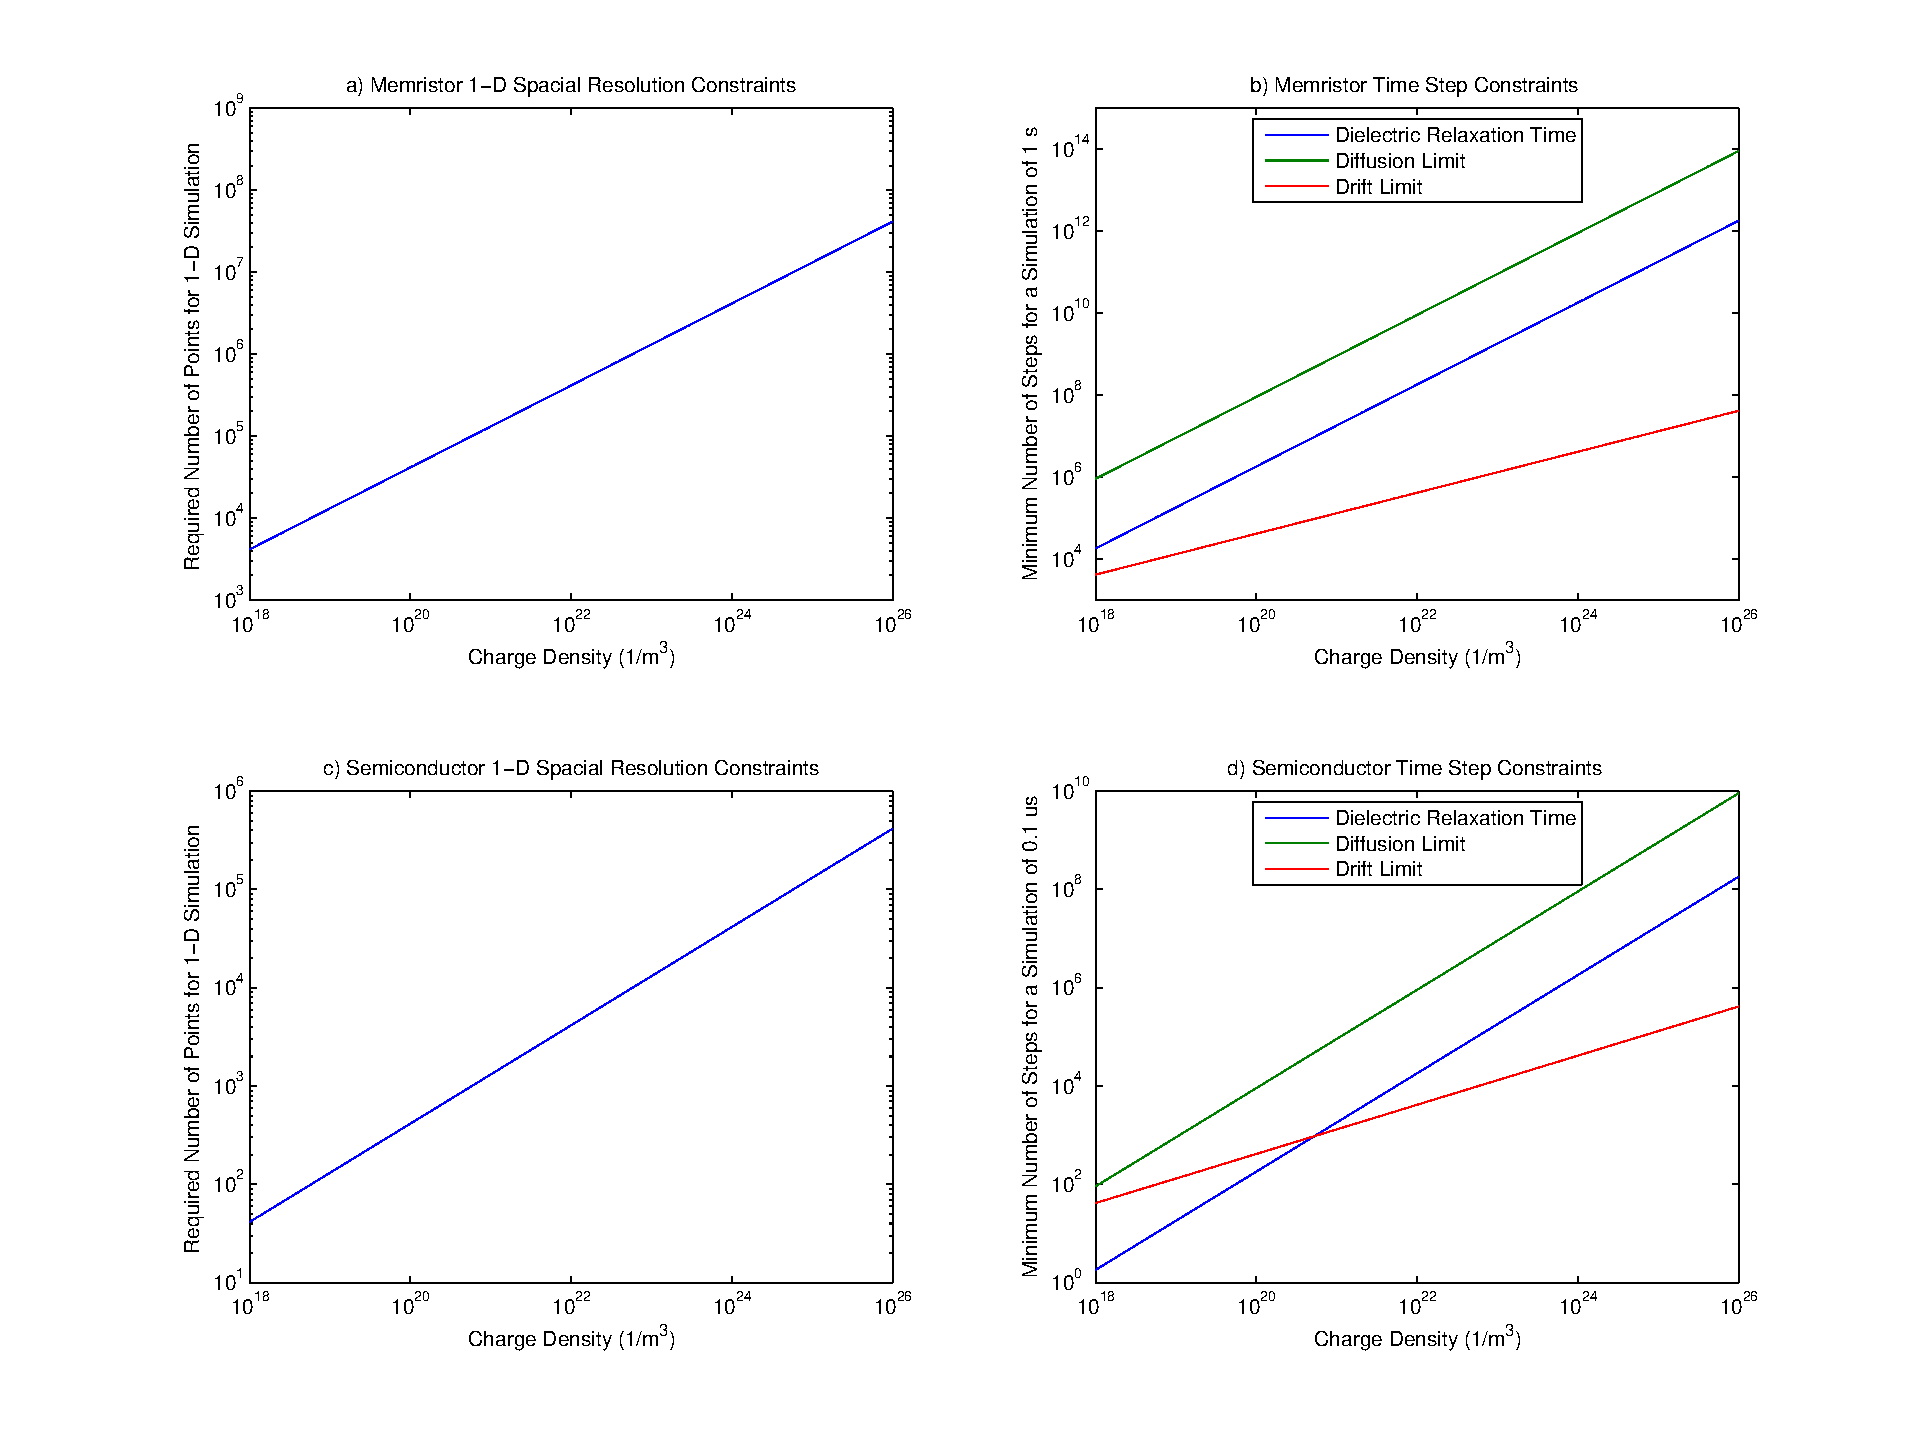
\includegraphics[scale=0.40]{SpaceTime}
\caption{} 
\label{}
\end{figure}


\clearpage
\section{Debye Length and Simulation Validity}
%-Steady state high concentration examples
%-Transient high concentration examples
\begin{figure}[!htp]
\centering
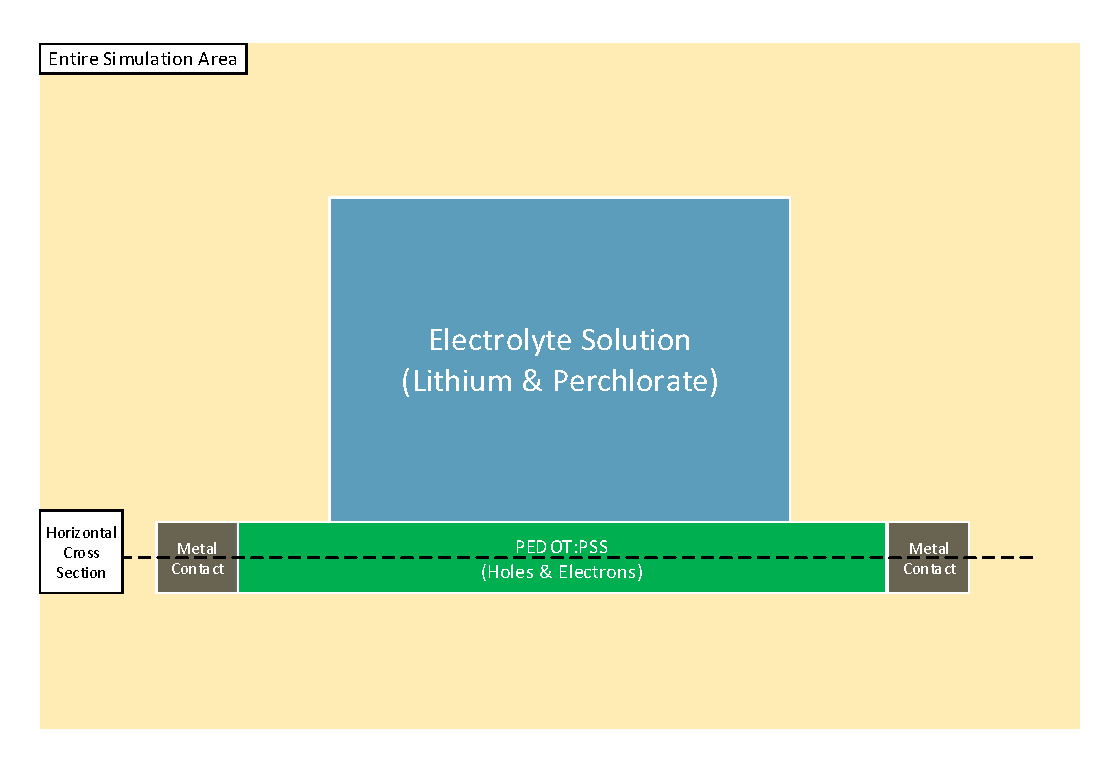
\includegraphics[scale=0.50]{Mem1}
\caption{} 
\label{}
\end{figure}


\subsection{1-D Horizontal Electrolyte}

\begin{figure}[!htp]
\centering
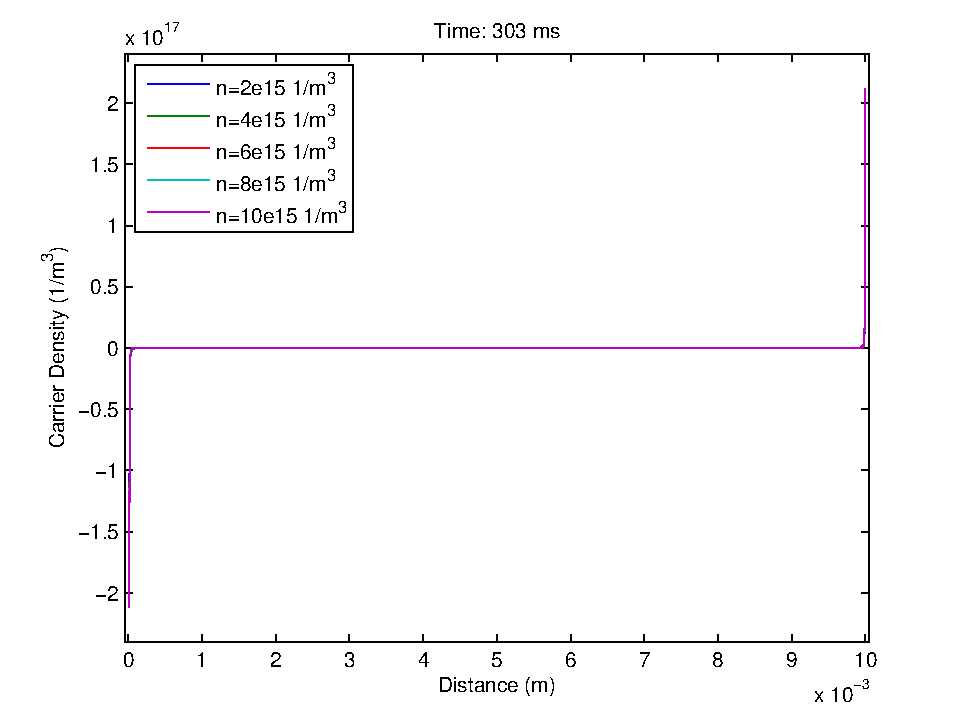
\includegraphics[scale=0.60]{Ex1NetQ_Time_All}
\caption{} 
\label{}
\end{figure}



\begin{landscape}
\begin{figure}[!htp]
\centering
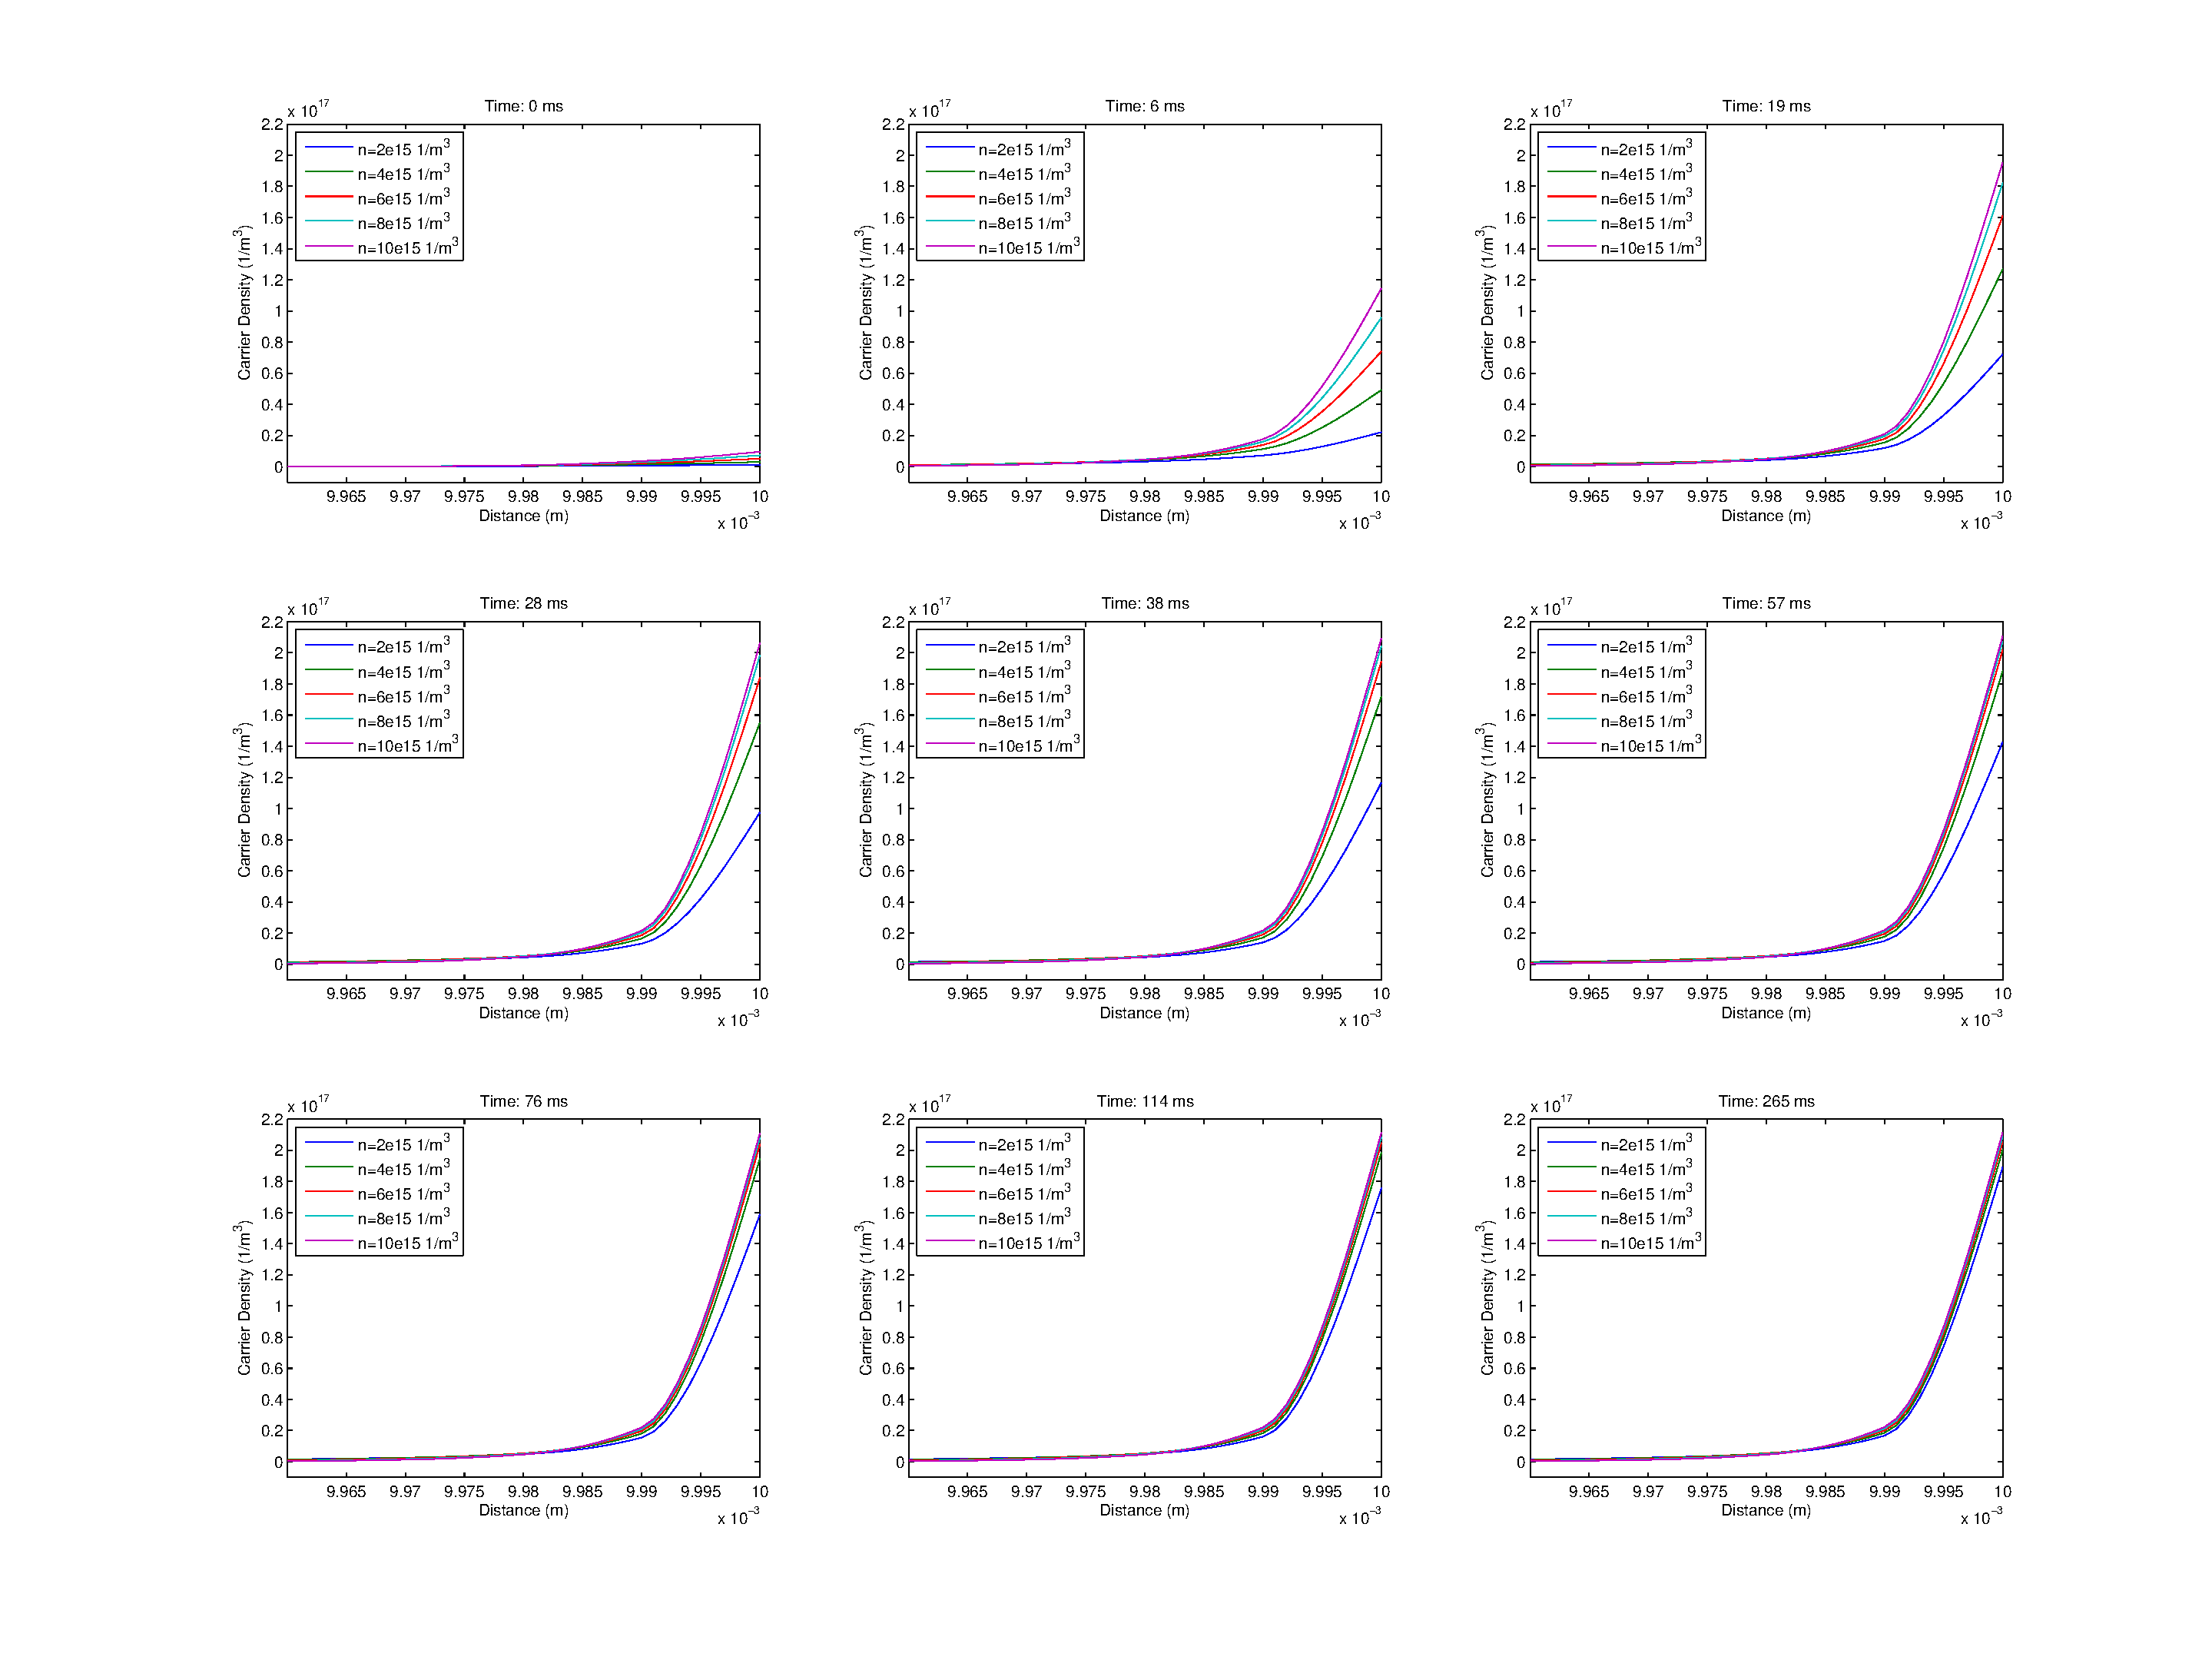
\includegraphics[scale=0.40]{Ex1NetQ_Time}
\caption{} 
\label{}
\end{figure}
\end{landscape}

\begin{landscape}
\begin{figure}[!htp]
\centering
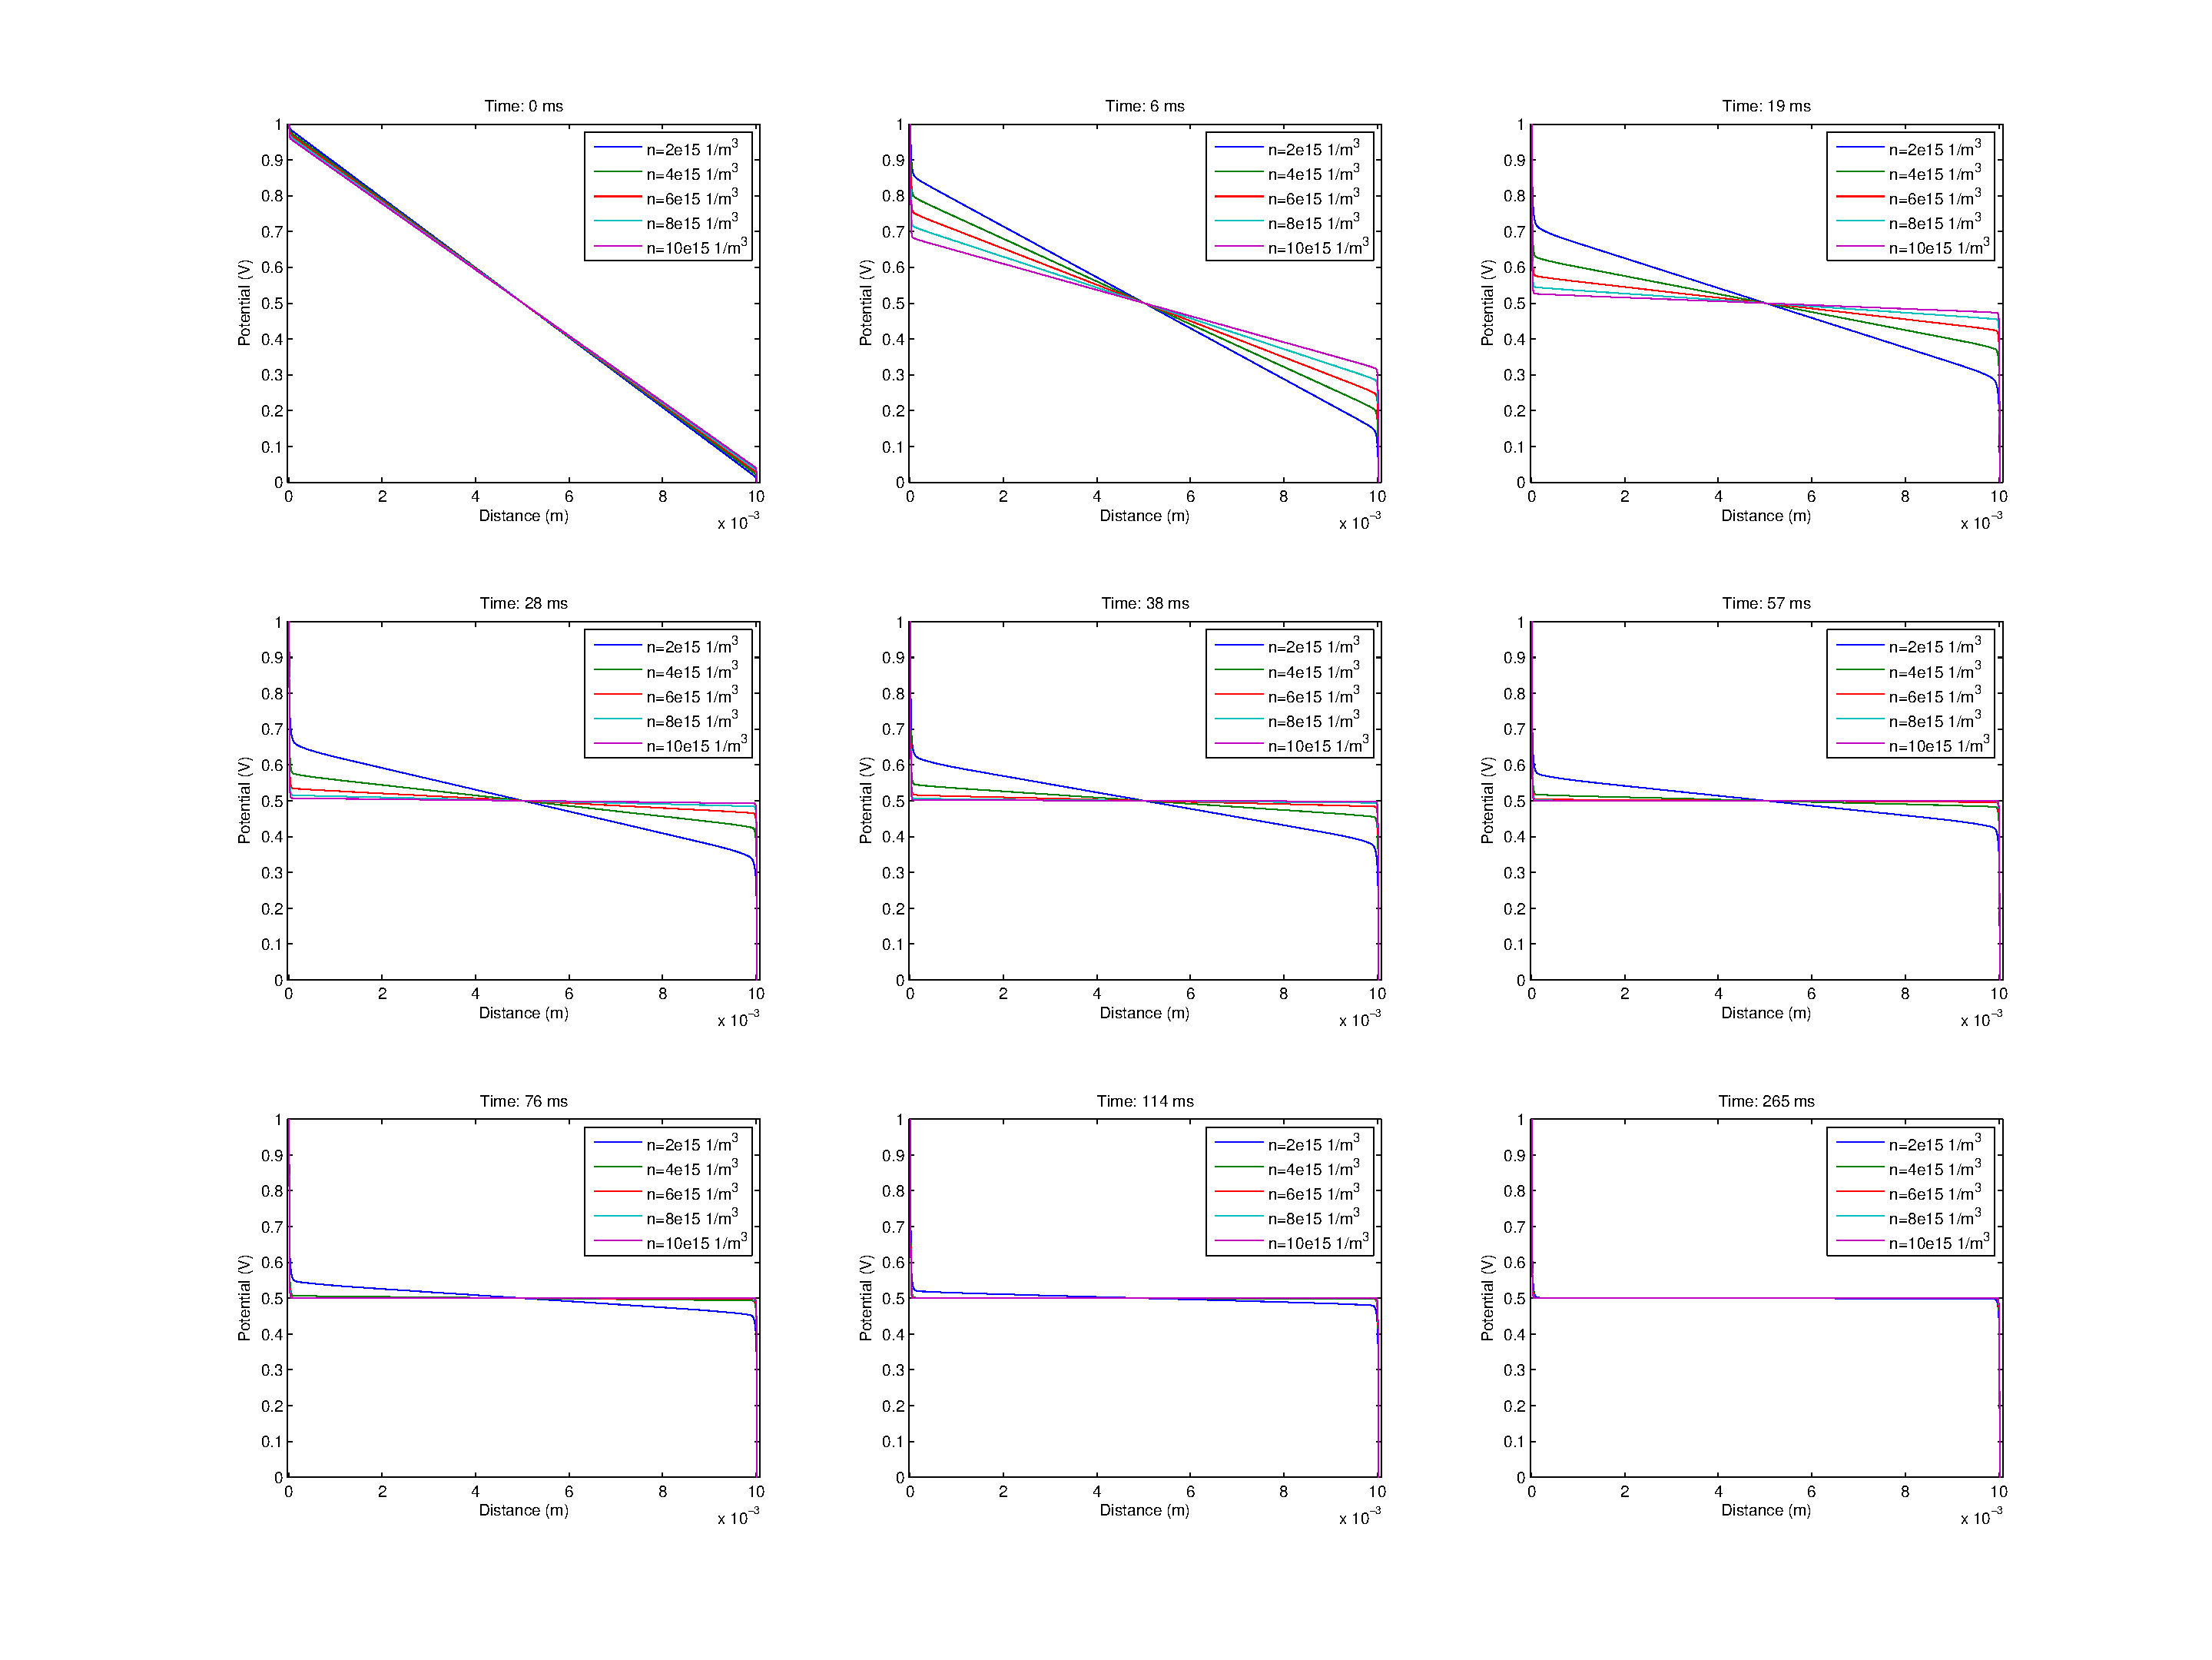
\includegraphics[scale=0.40]{Ex1V_Time}
\caption{} 
\label{}
\end{figure}
\end{landscape}

\begin{landscape}
\begin{figure}[!htp]
\centering
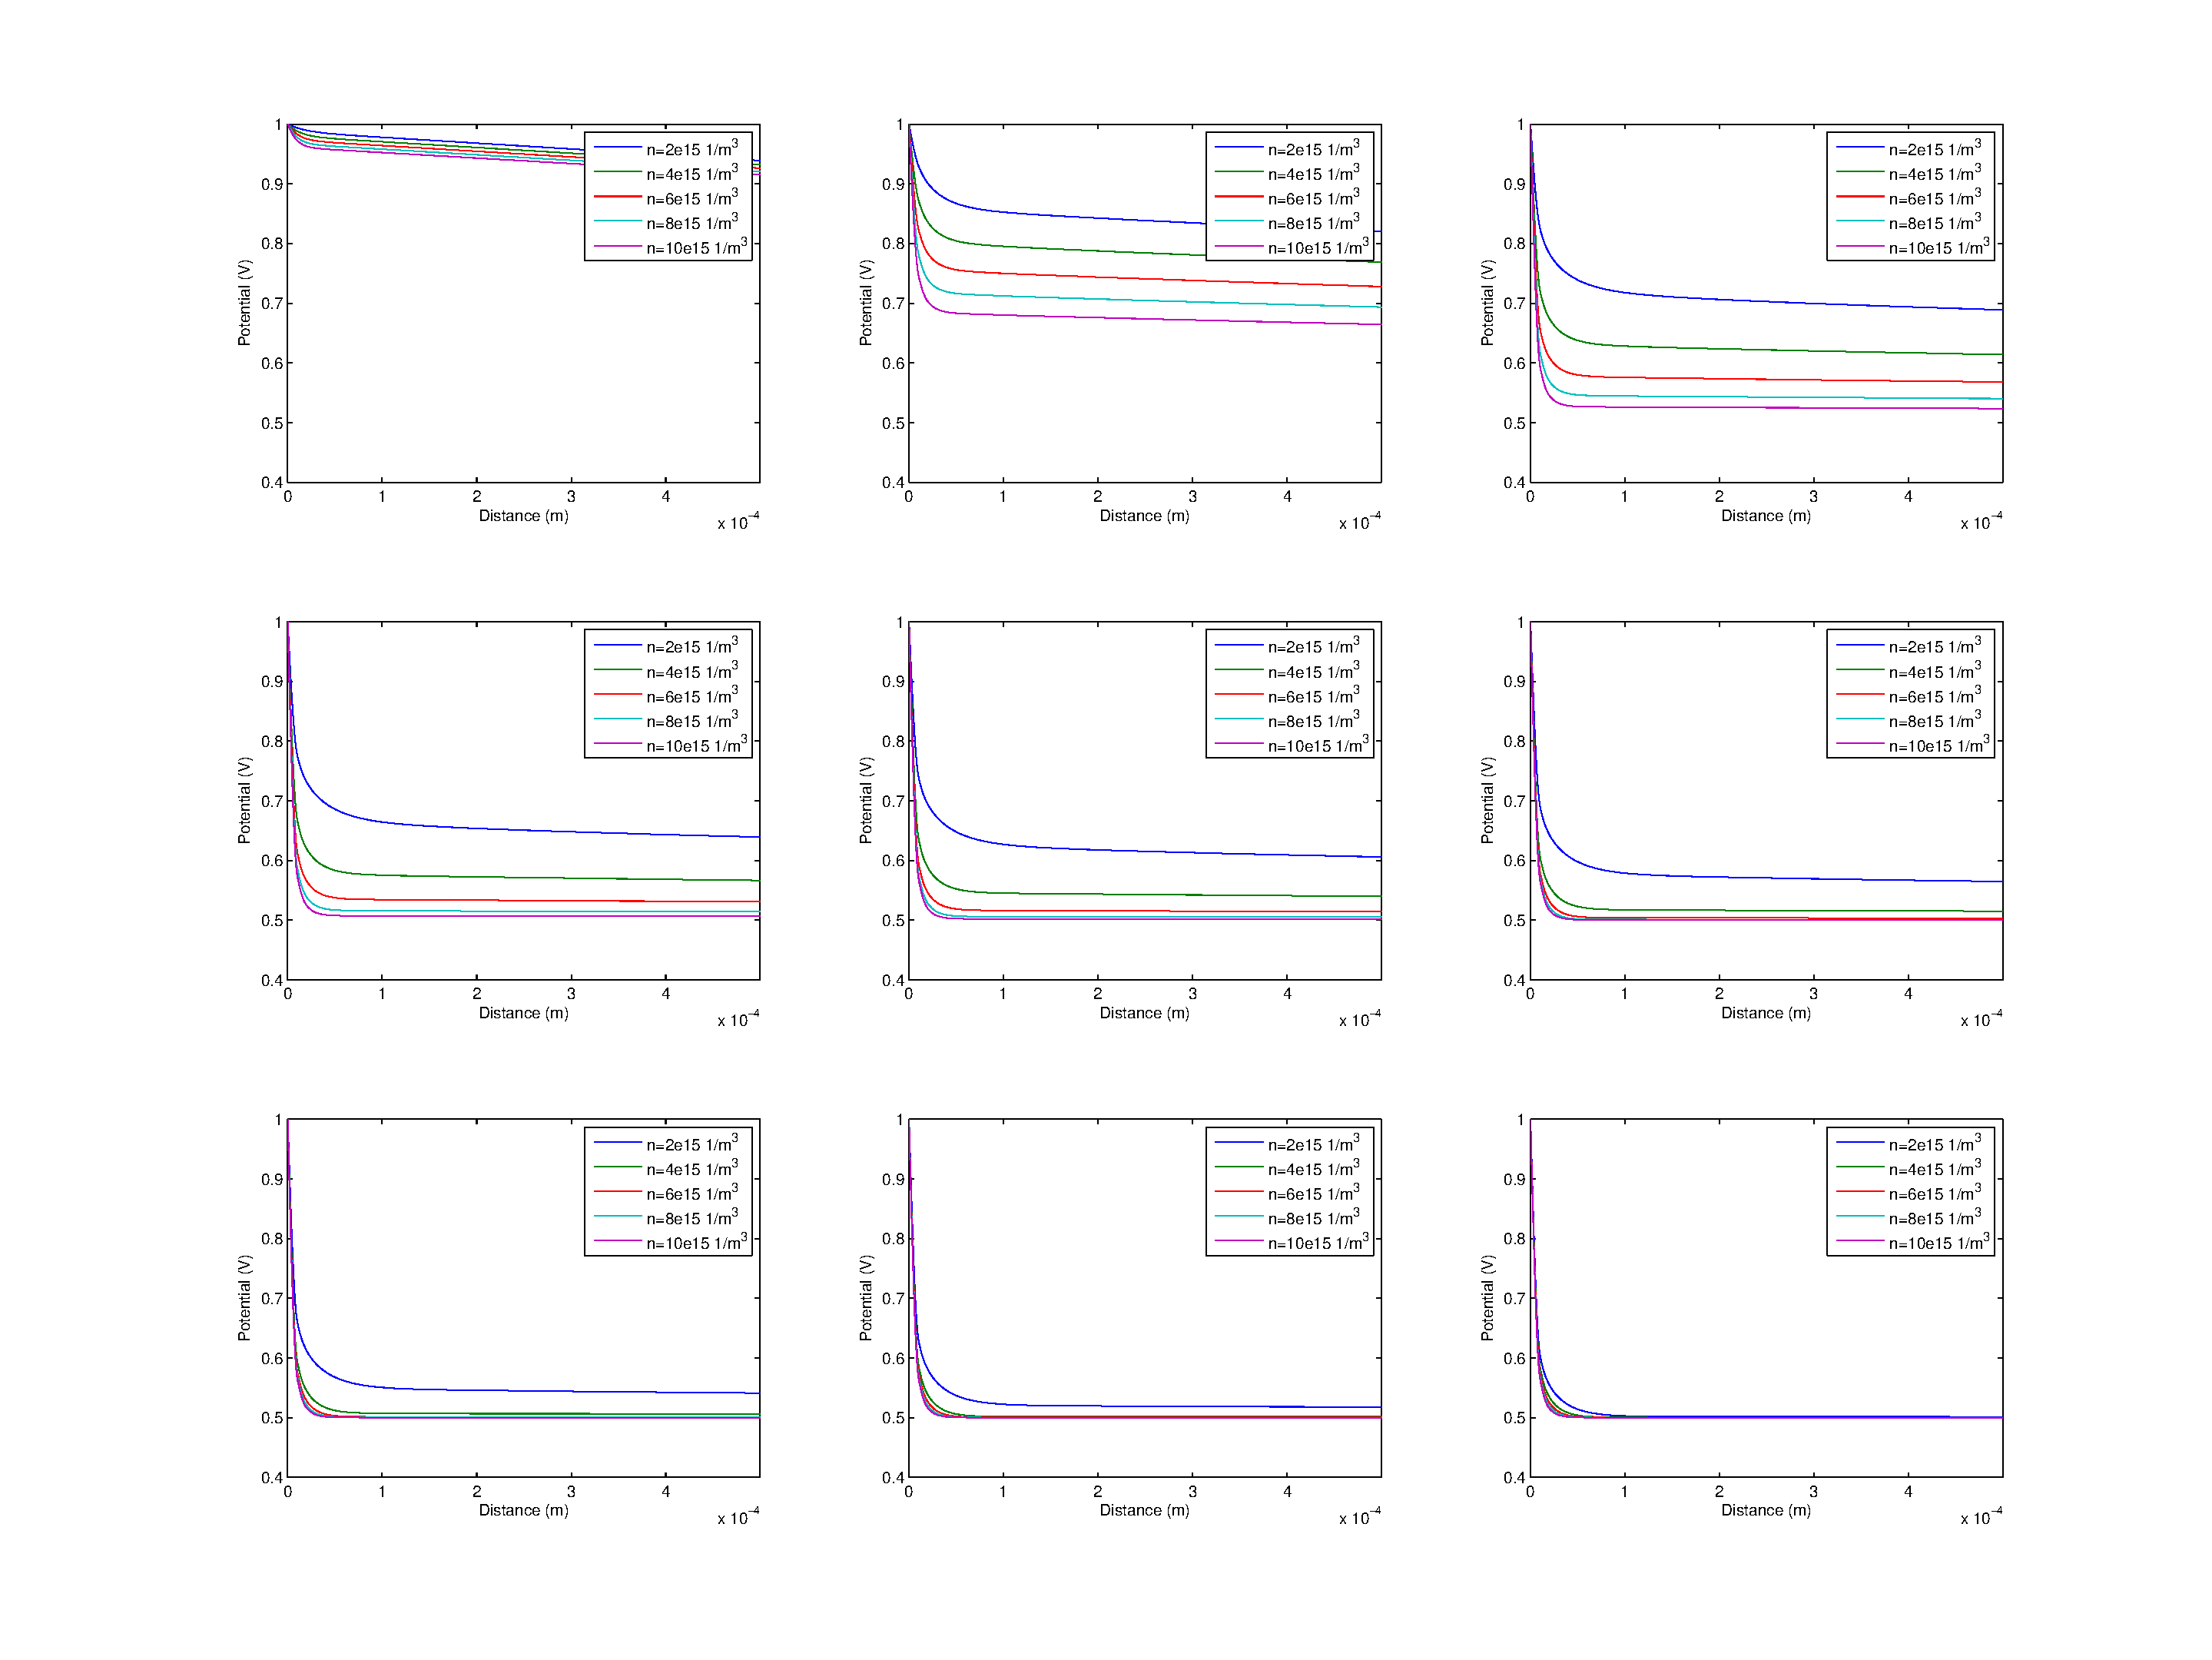
\includegraphics[scale=0.40]{Ex1V_Time2}
\caption{} 
\label{}
\end{figure}
\end{landscape}

\clearpage
\subsection{1-D ?}
\begin{figure}[!htp]
\centering
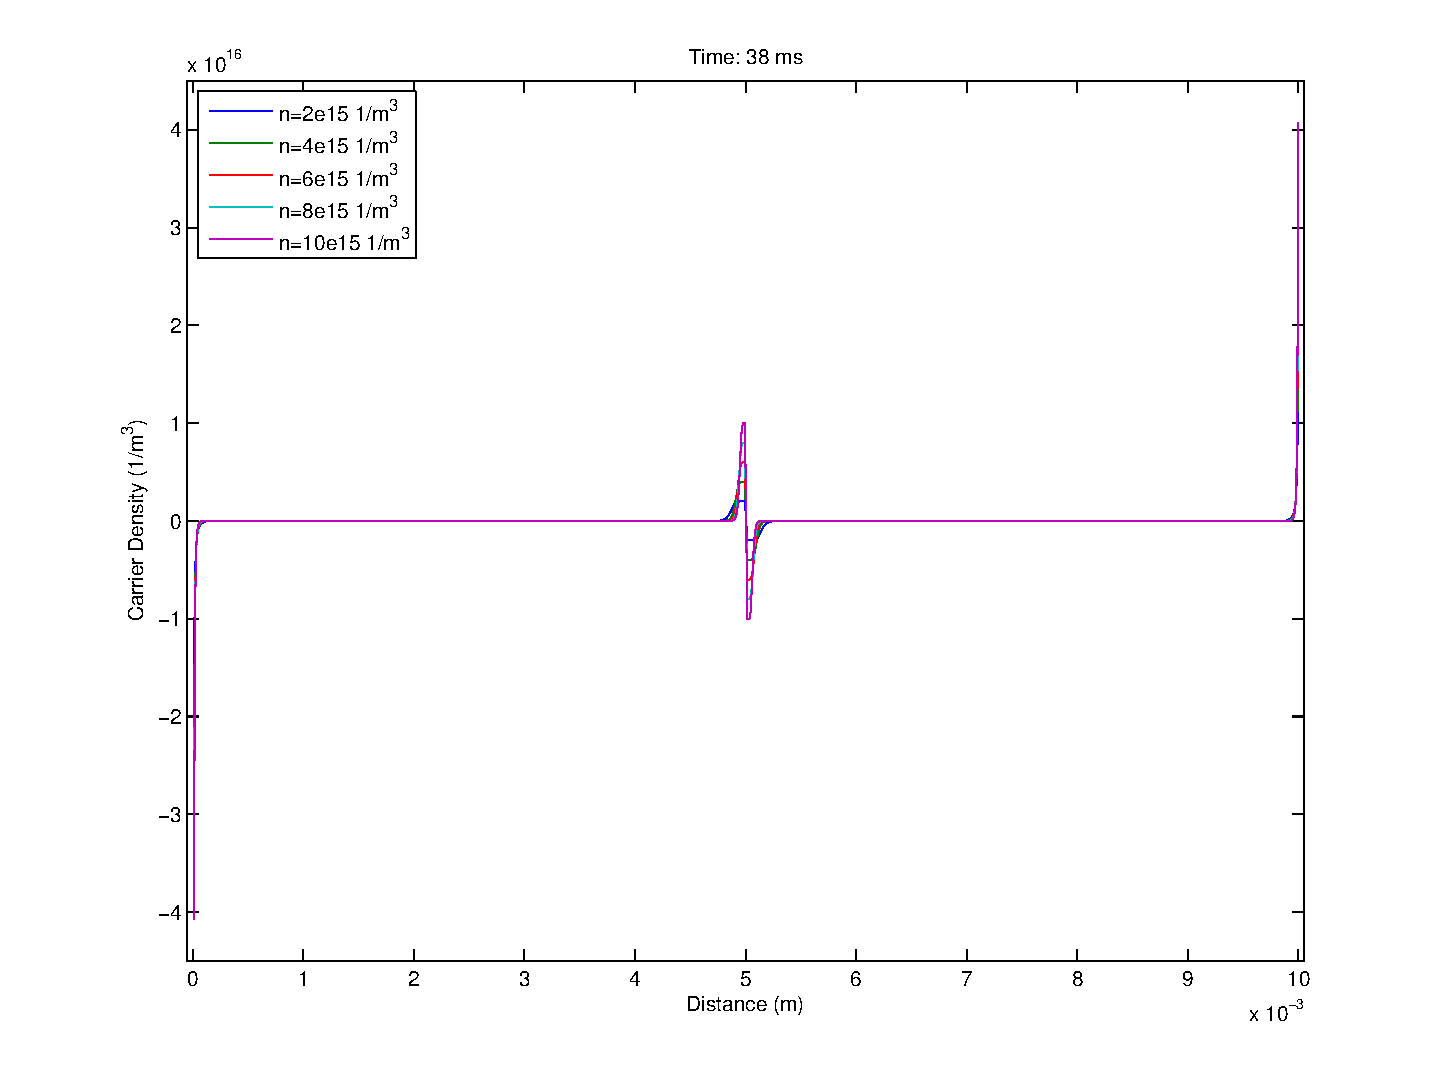
\includegraphics[scale=0.60]{Ex2NetQ_Time_All}
\caption{} 
\label{}
\end{figure}


\begin{landscape}
\begin{figure}[!htp]
\centering
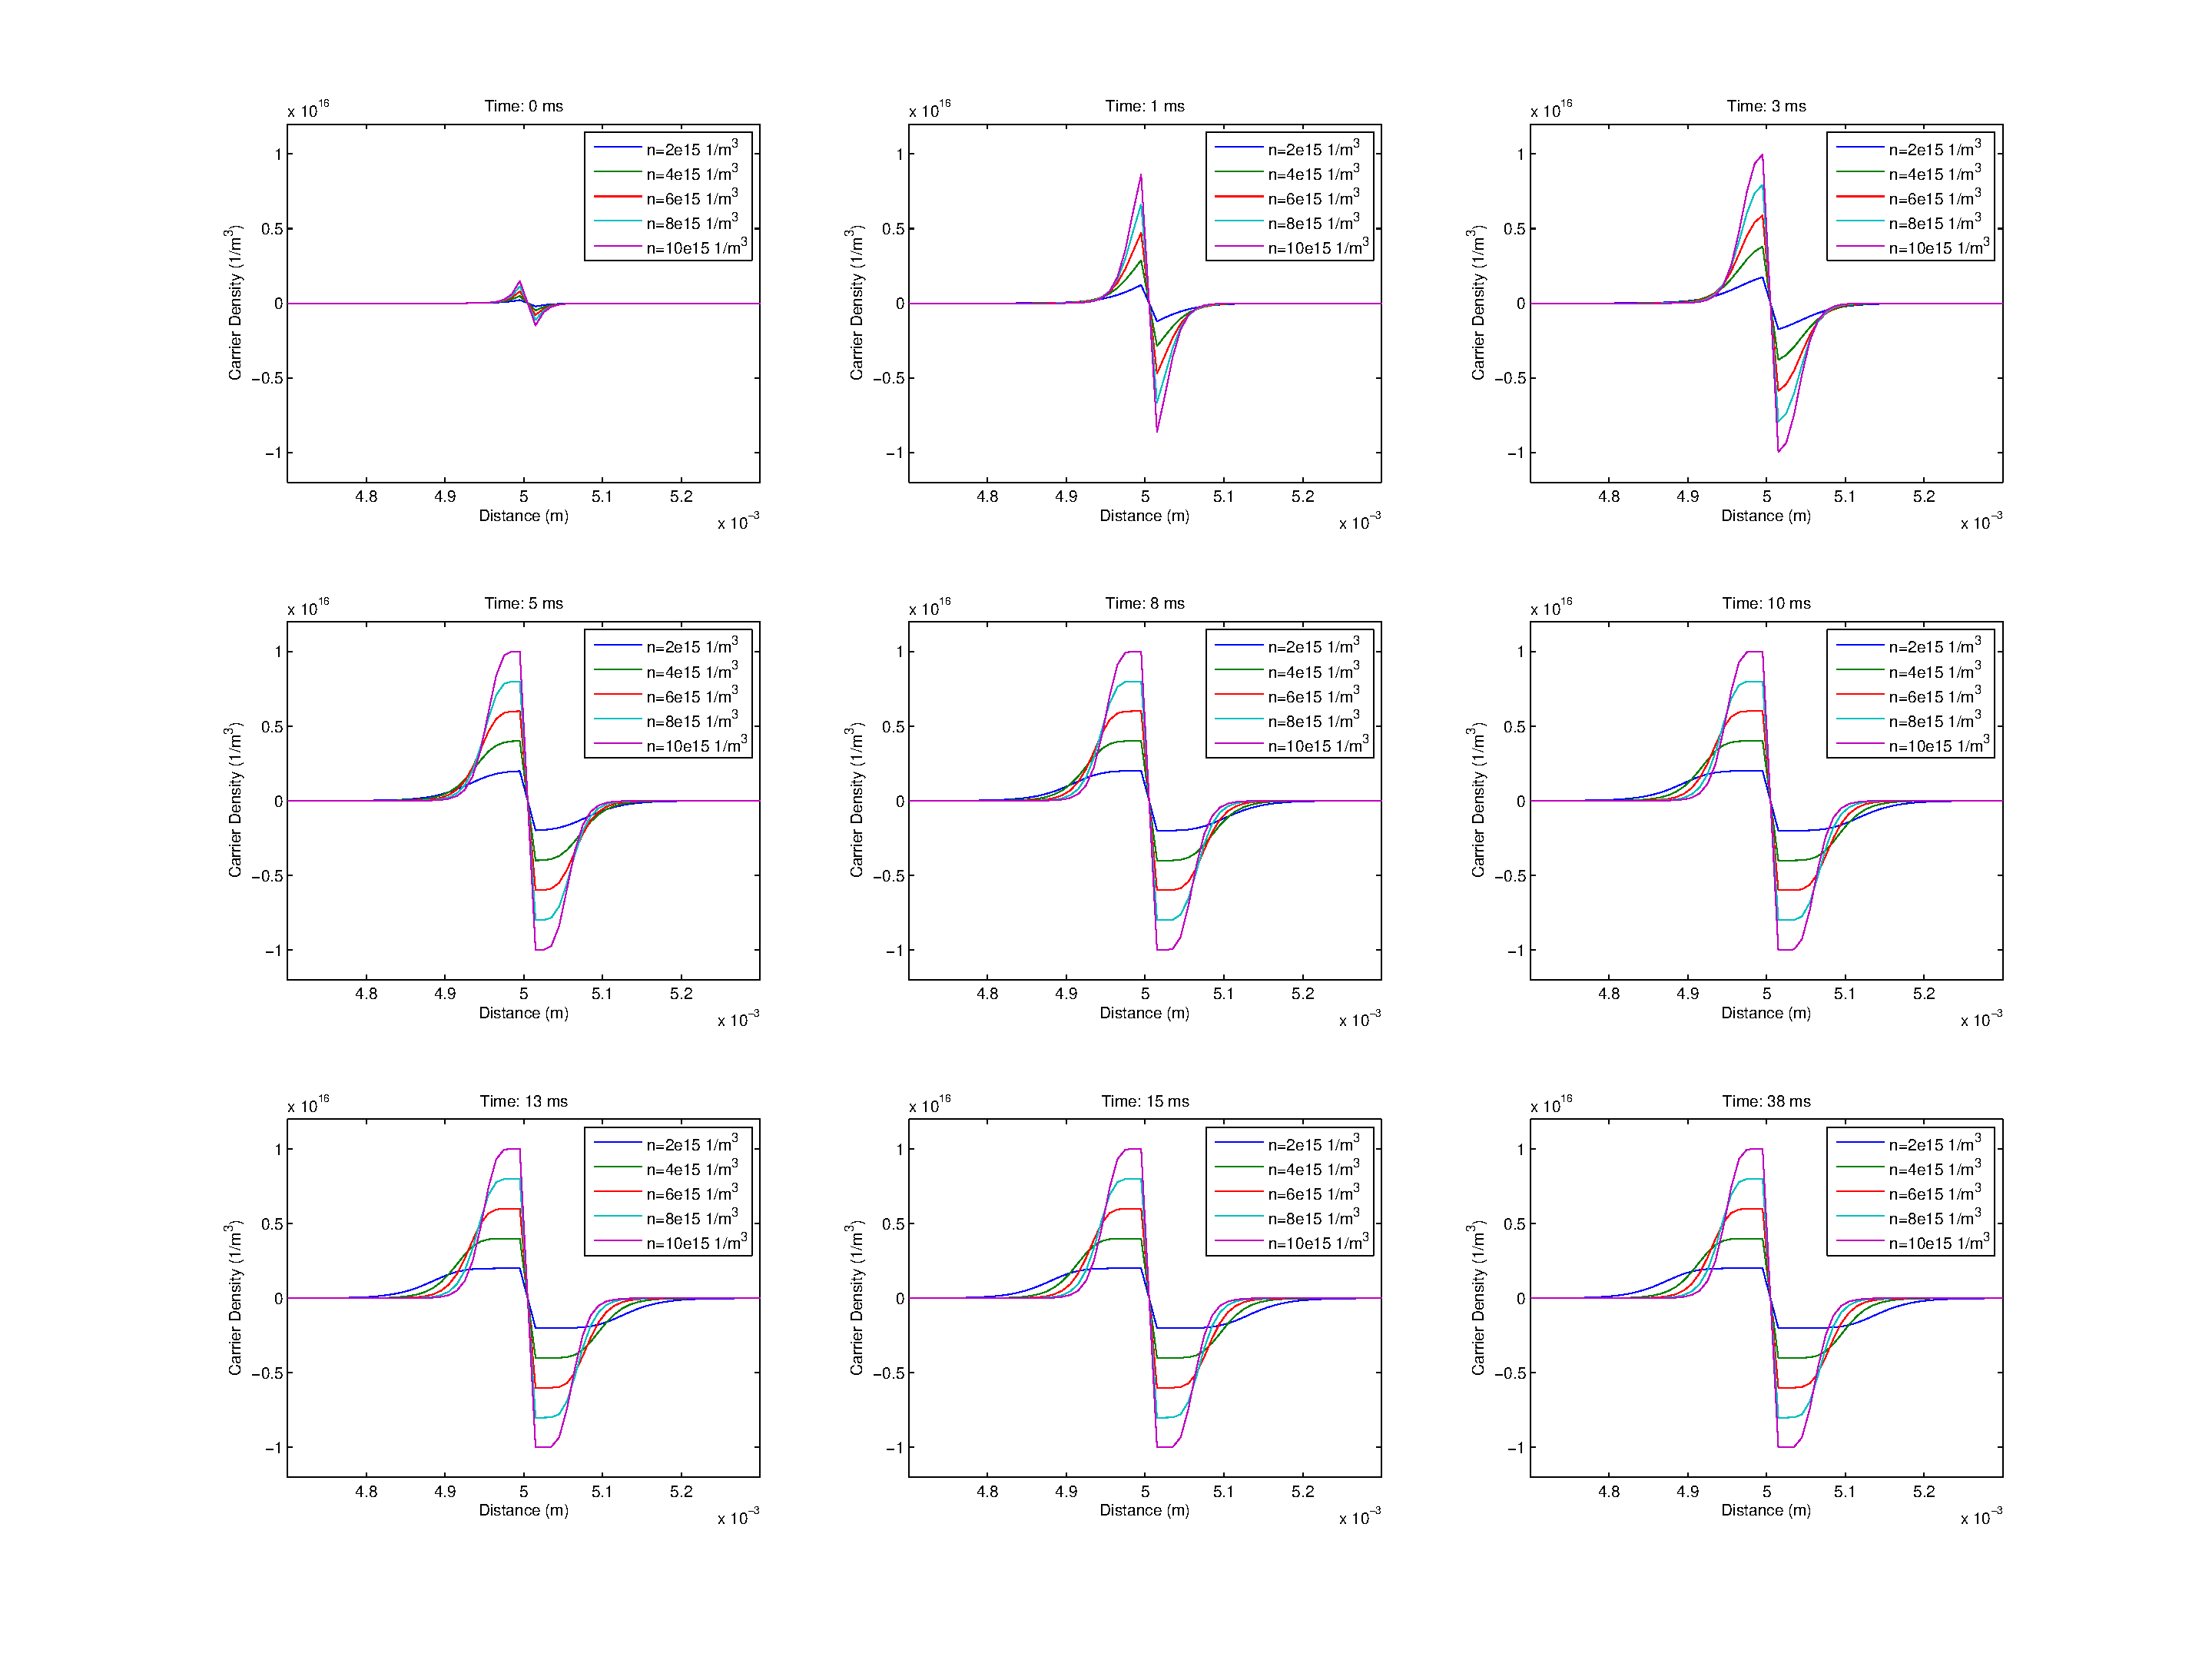
\includegraphics[scale=0.40]{Ex2NetQ_Time}
\caption{} 
\label{}
\end{figure}
\end{landscape}

\begin{landscape}
\begin{figure}[!htp]
\centering
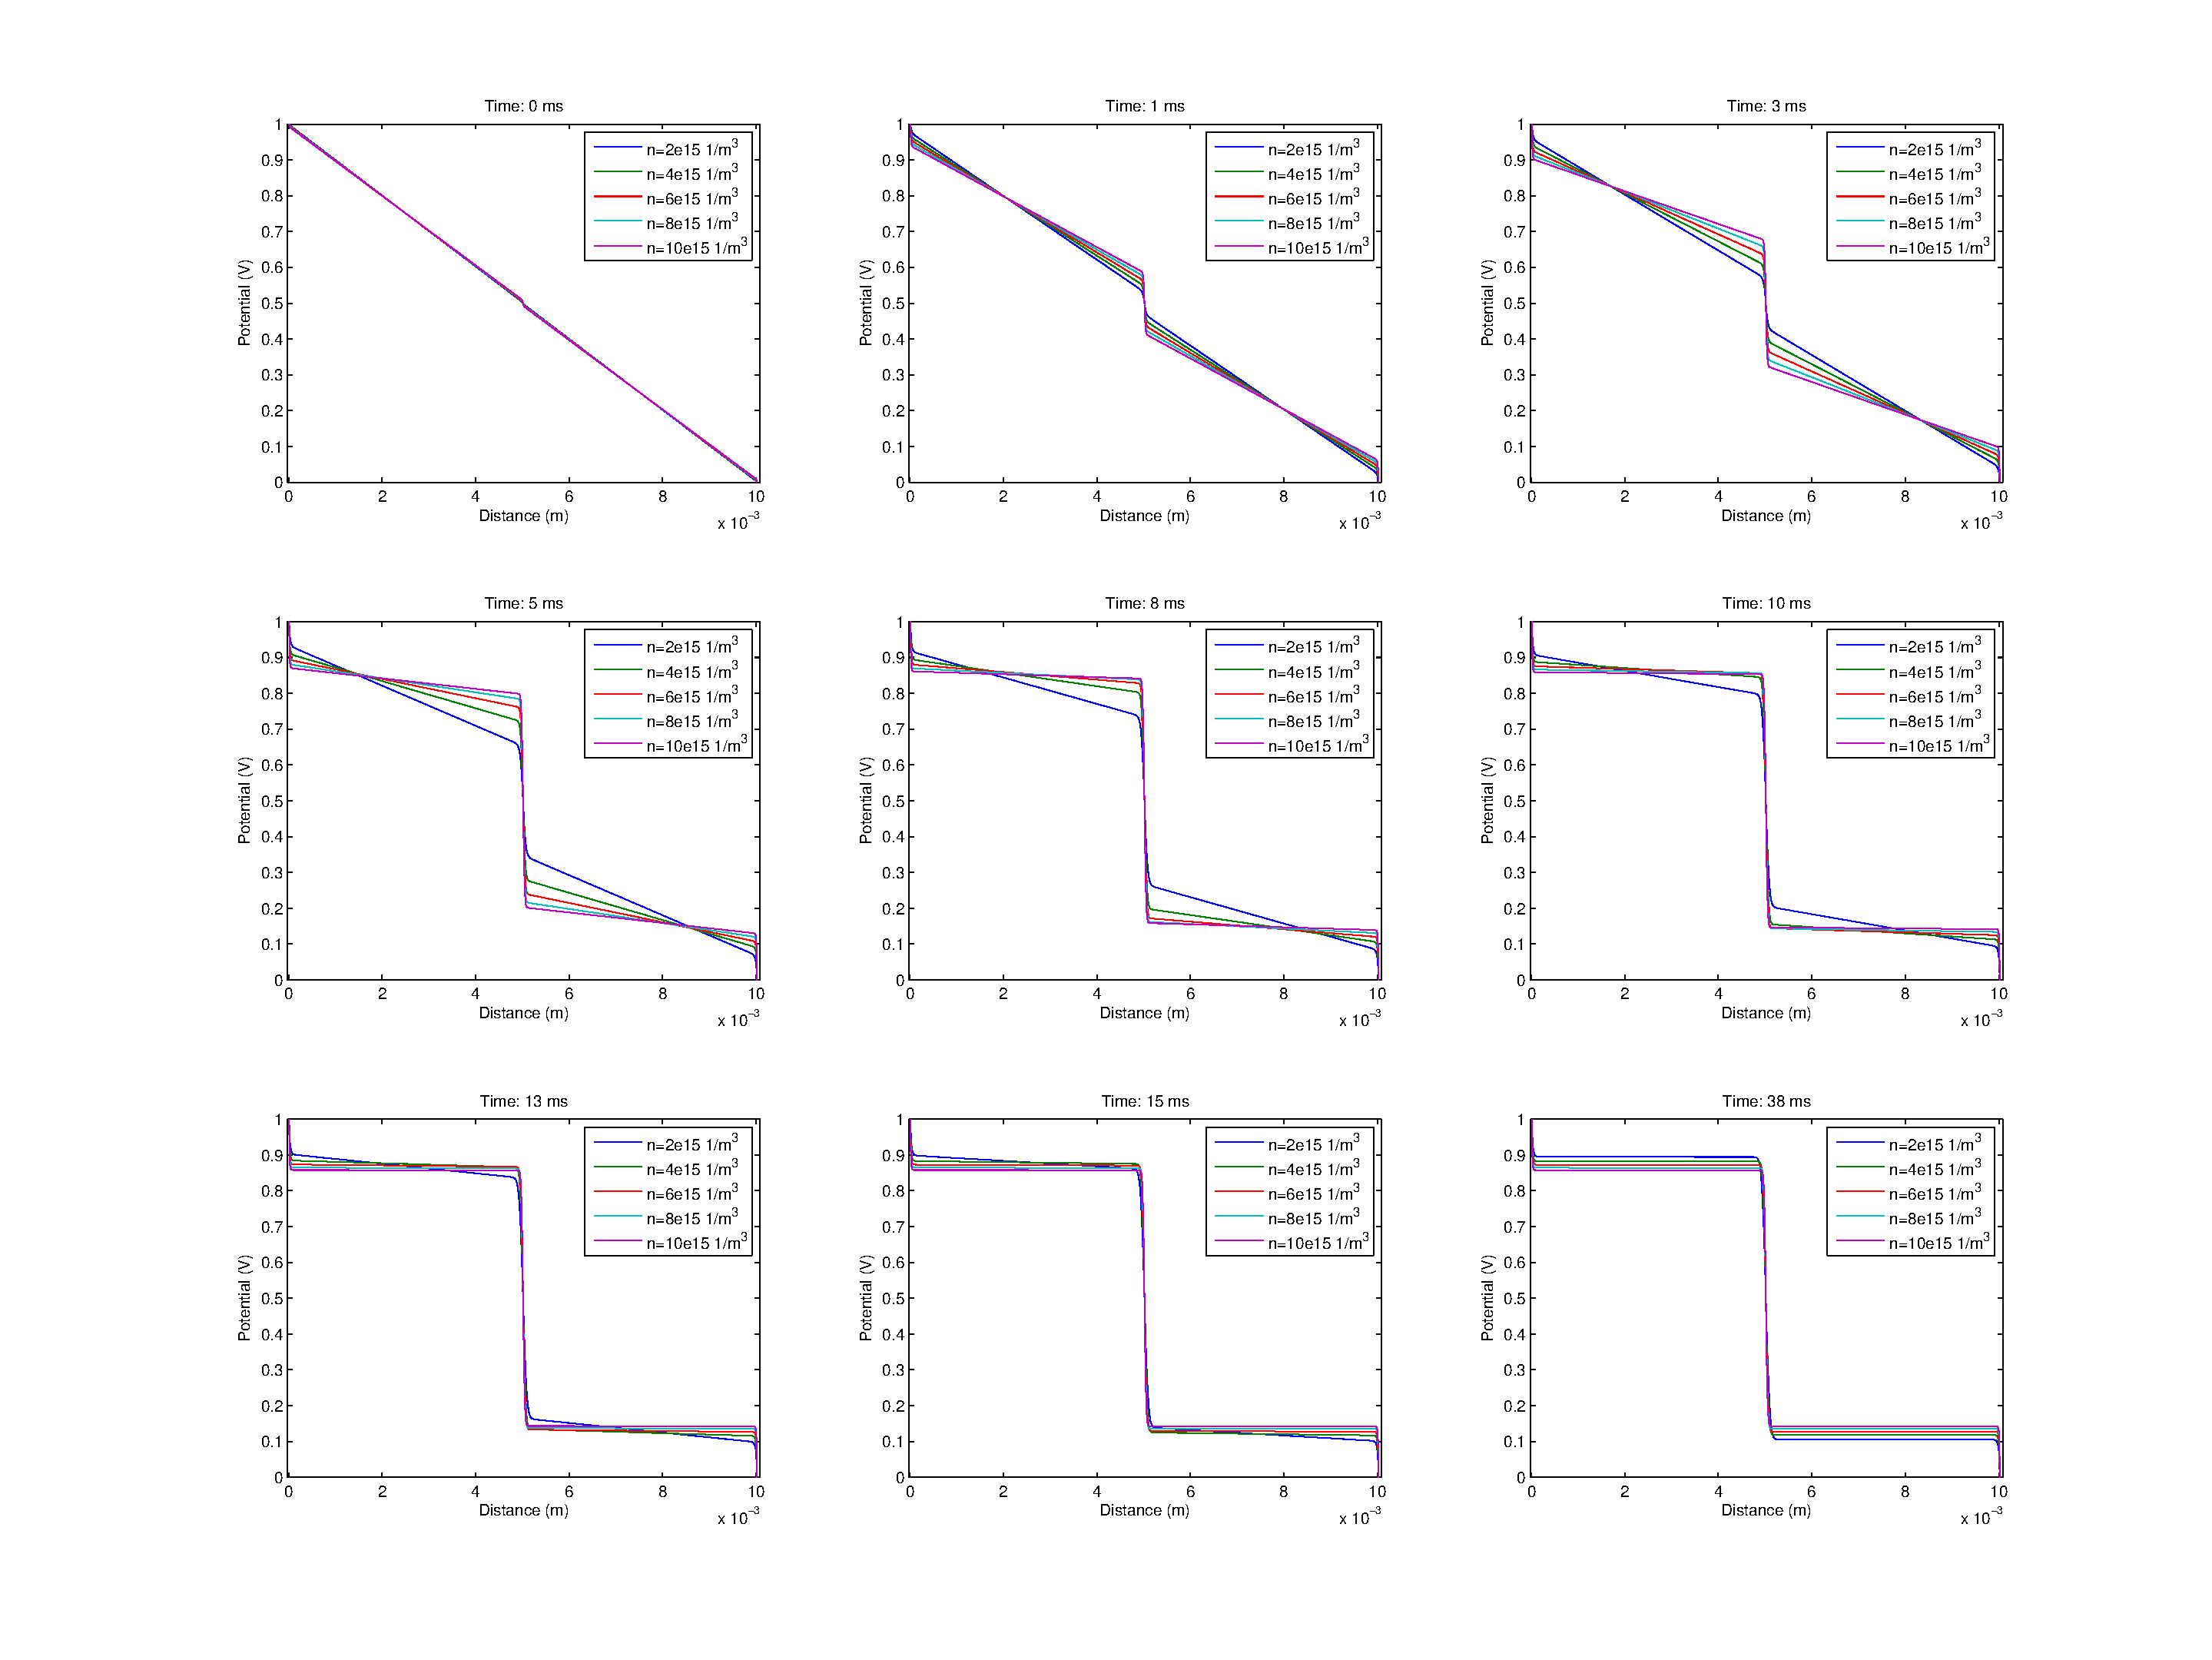
\includegraphics[scale=0.40]{Ex2V_Time}
\caption{} 
\label{}
\end{figure}
\end{landscape}

\clearpage
\subsection{1-D Horizontal PEDOT:PSS with Notch}
\begin{figure}[!htp]
\centering
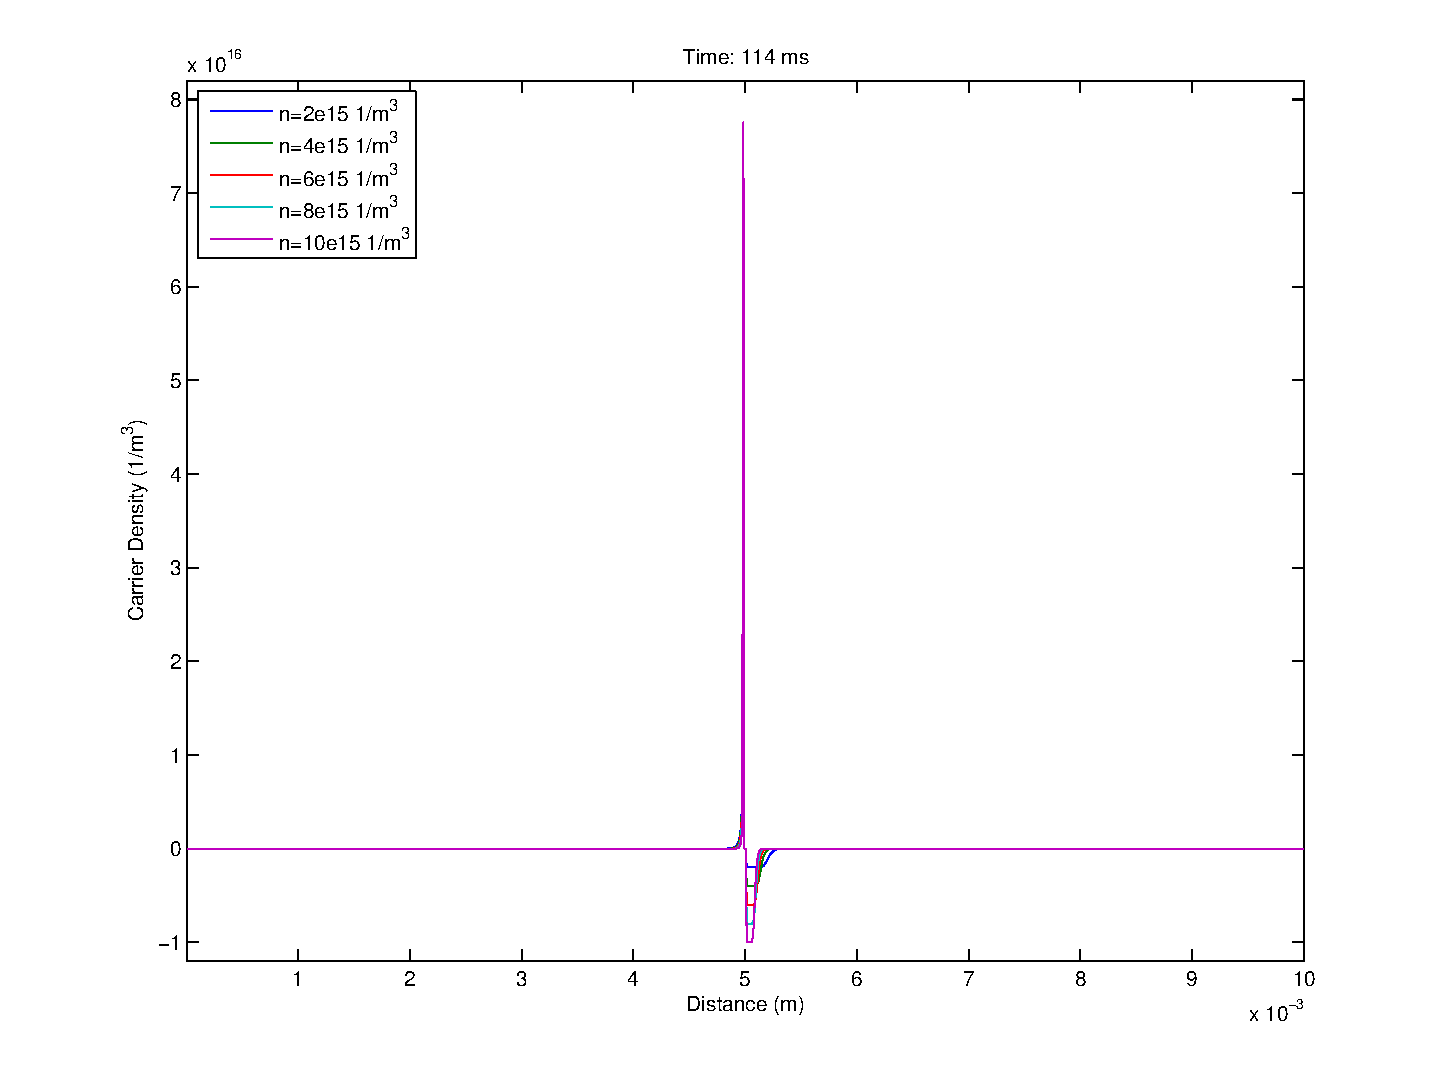
\includegraphics[scale=0.60]{Ex3NetQ_Time_All}
\caption{} 
\label{}
\end{figure}


\begin{landscape}
\begin{figure}[!htp]
\centering
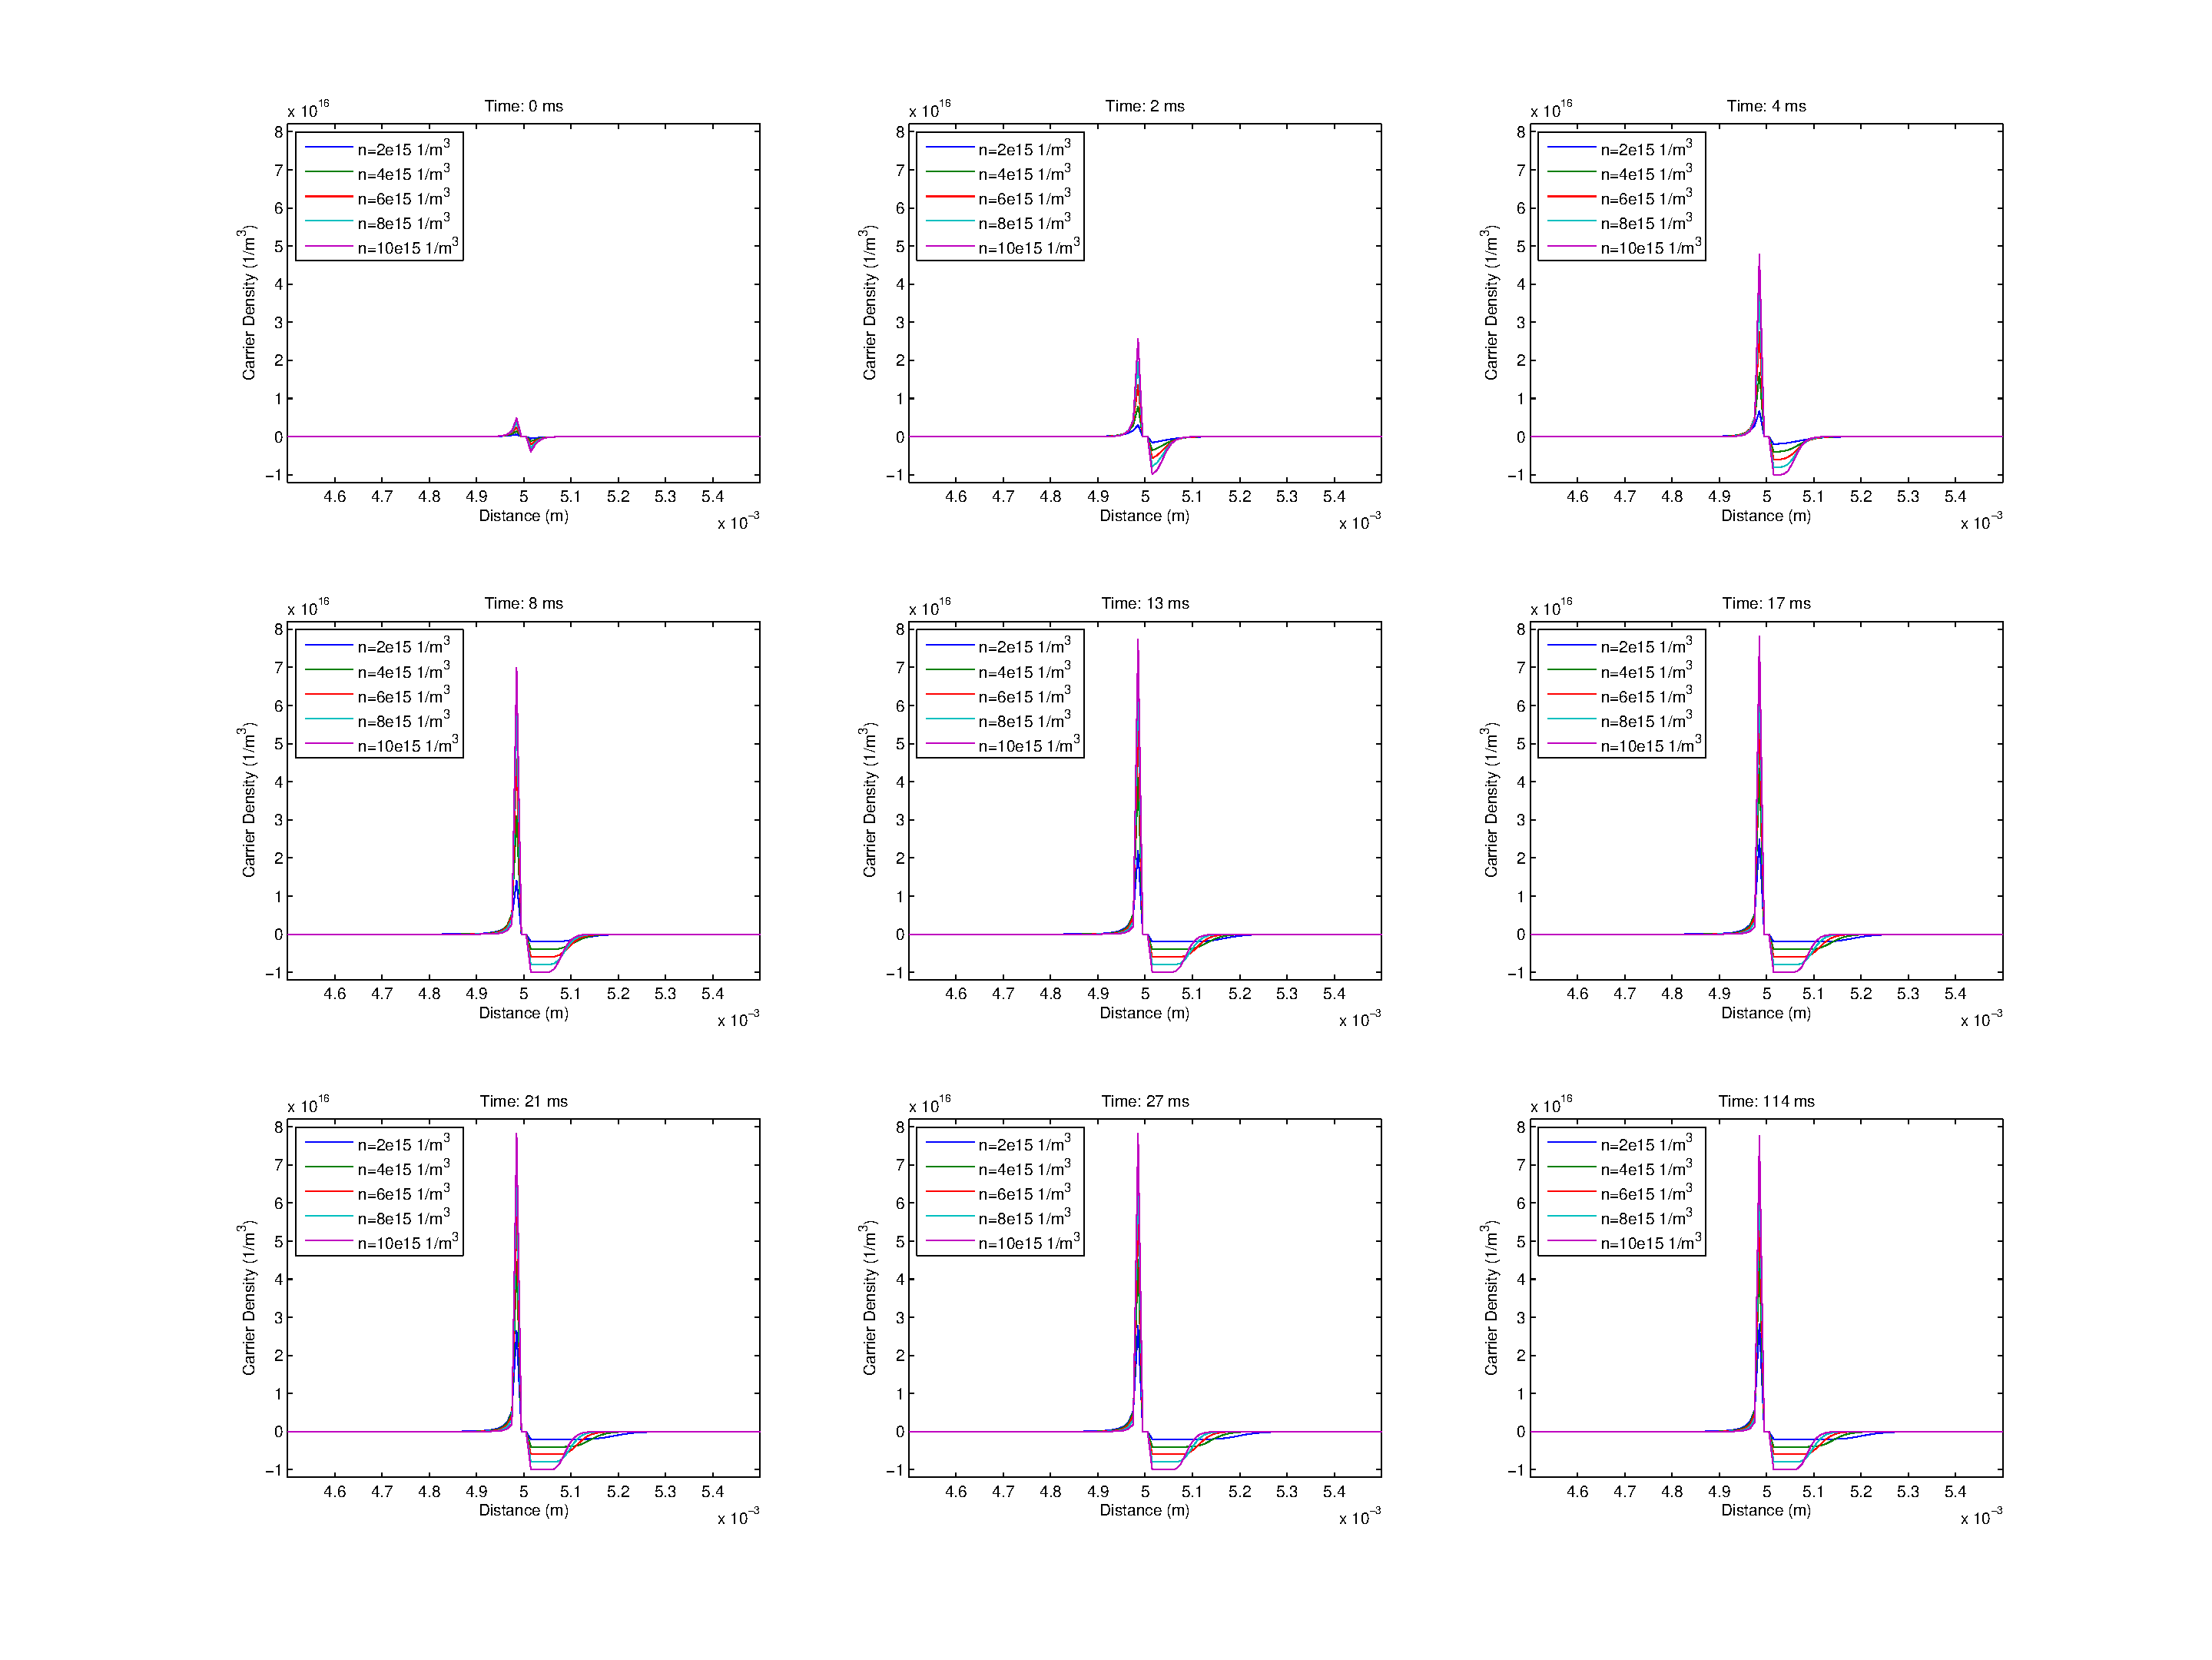
\includegraphics[scale=0.40]{Ex3NetQ_Time}
\caption{} 
\label{}
\end{figure}
\end{landscape}

\begin{landscape}
\begin{figure}[!htp]
\centering
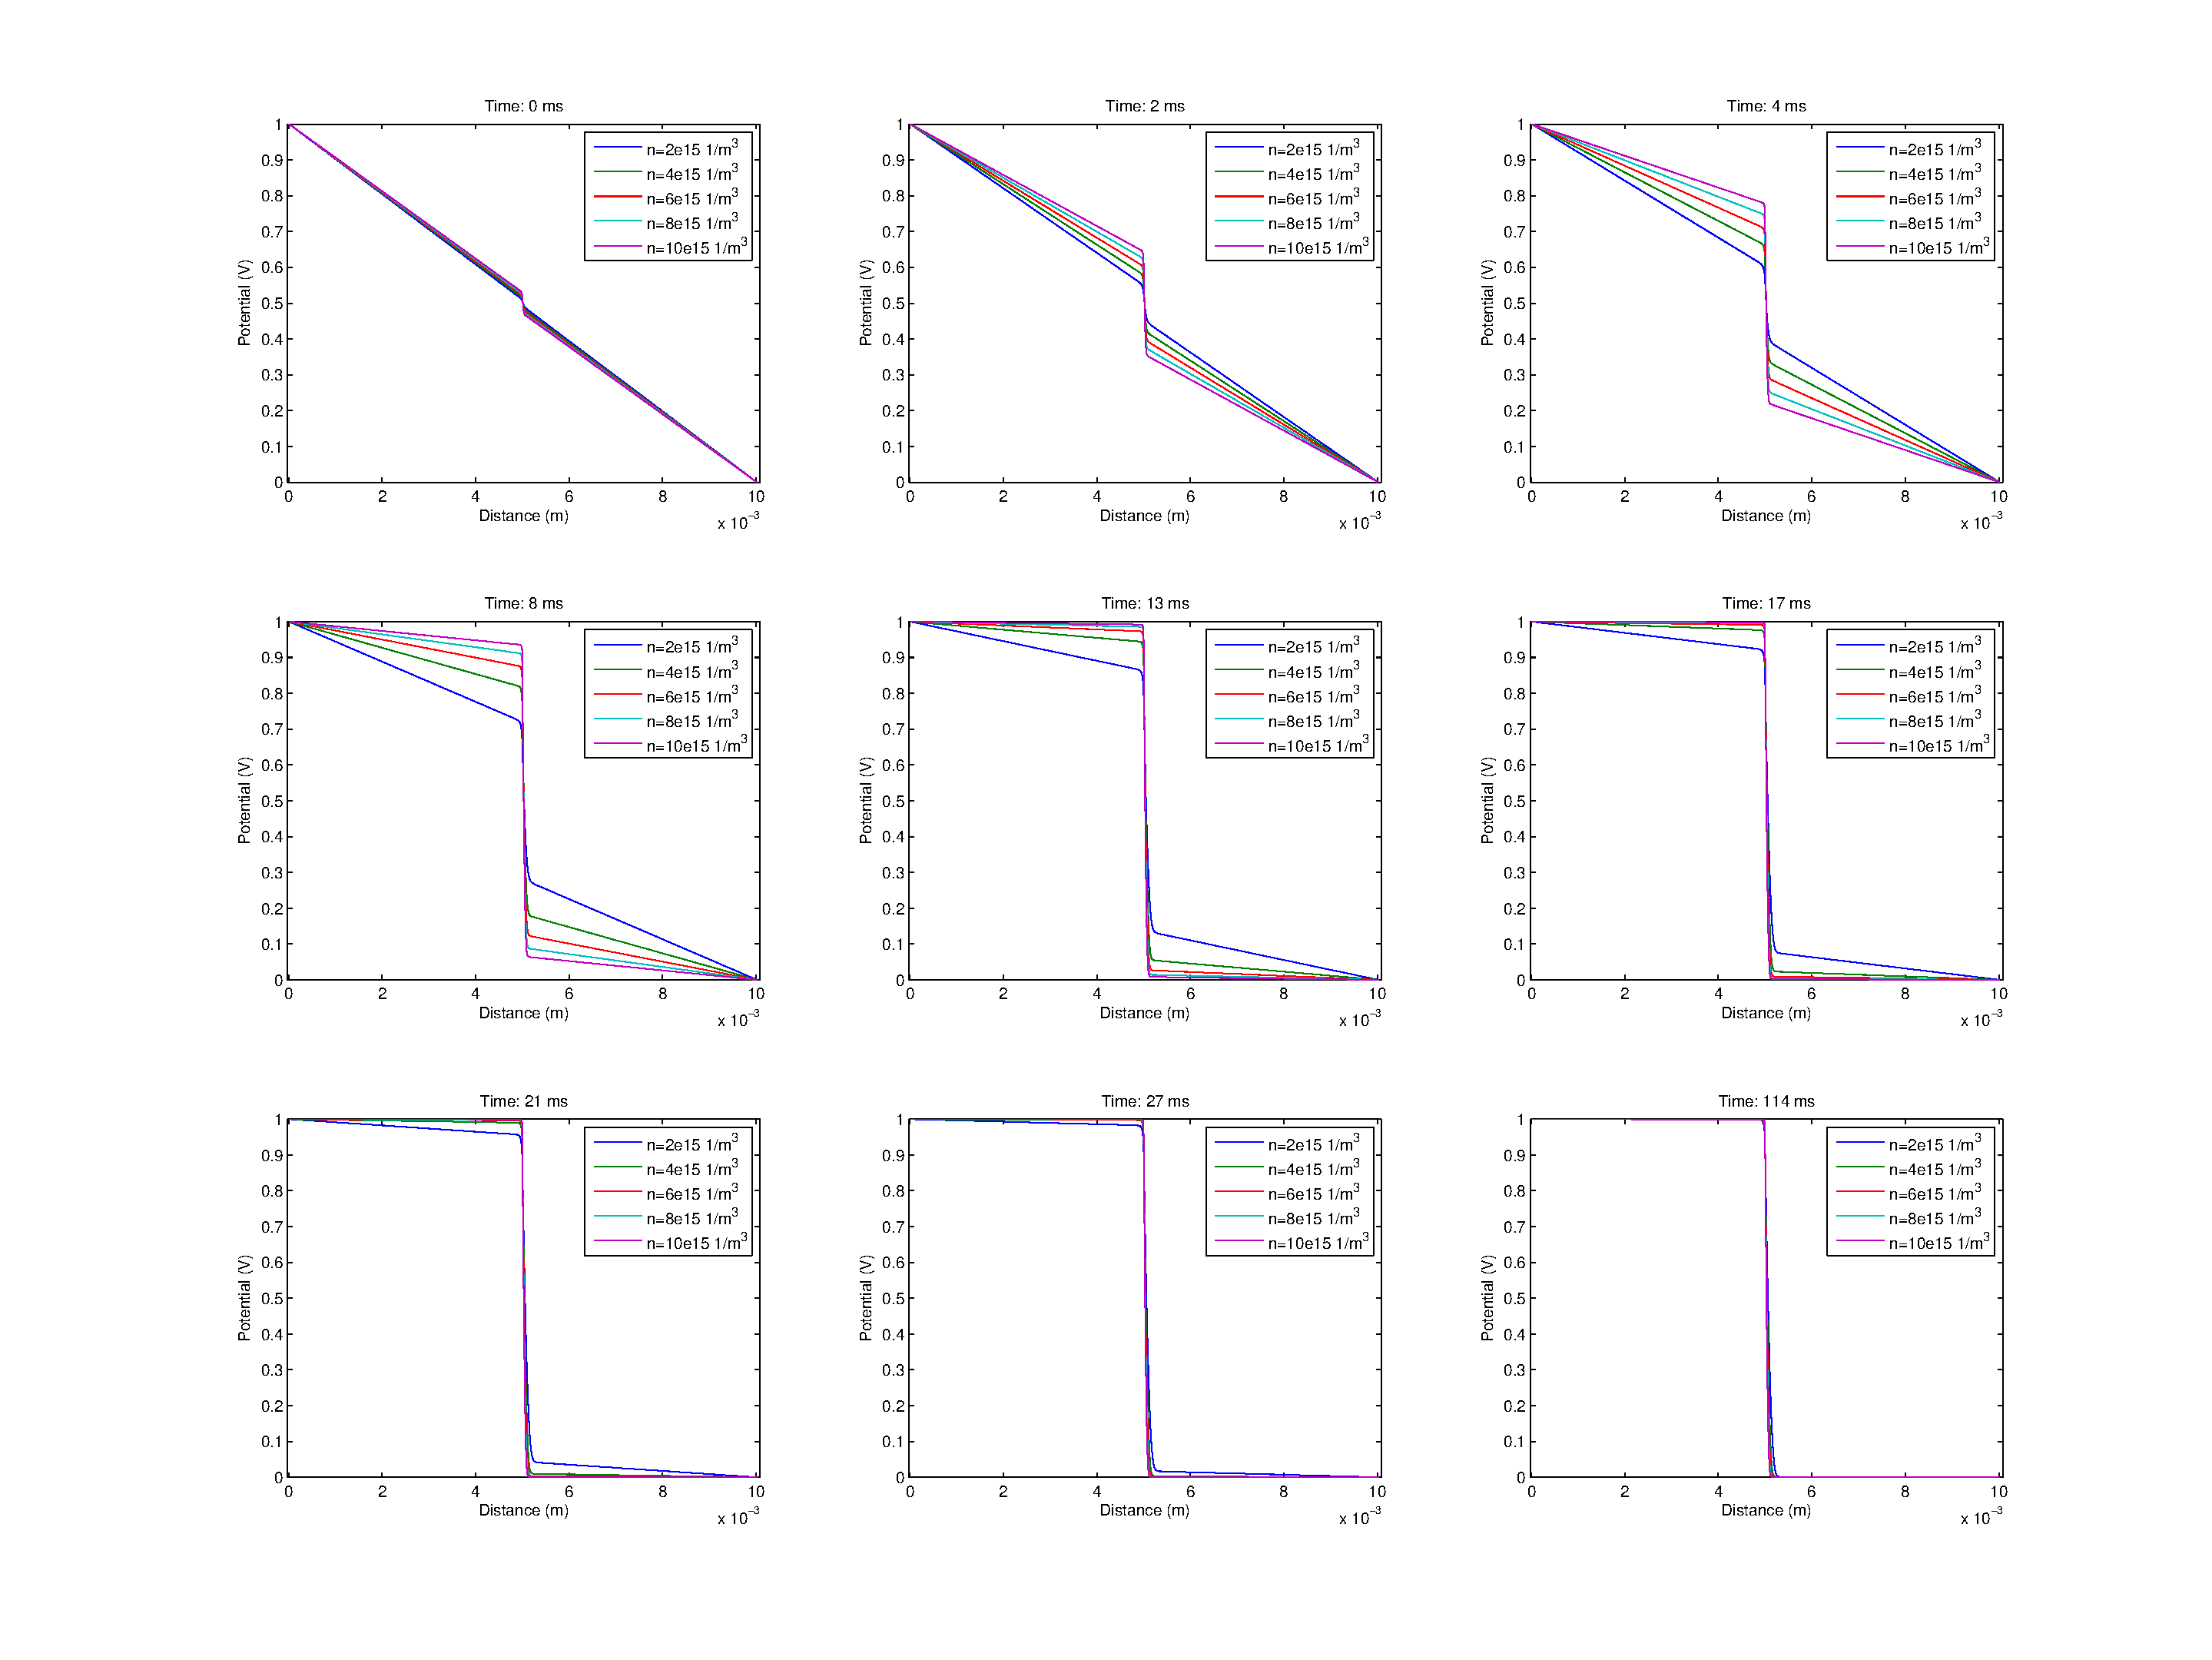
\includegraphics[scale=0.40]{Ex3V_Time}
\caption{} 
\label{}
\end{figure}
\end{landscape}

\clearpage
\subsection{1-D Vertical Electrolyte/PEDOT Interface}


\begin{figure}[!htp]
\centering
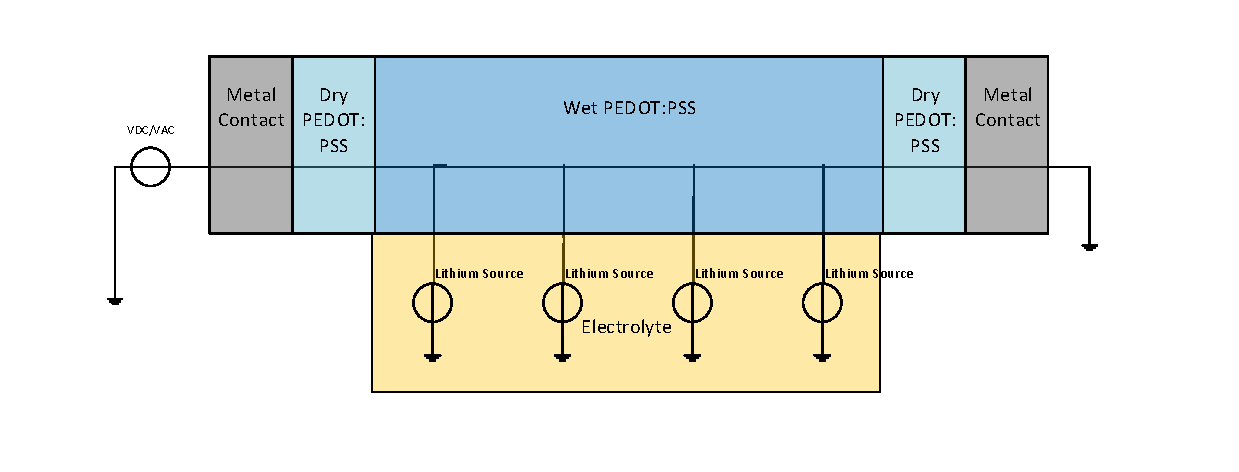
\includegraphics[scale=0.74]{1DMem}
\caption{} 
\label{}
\end{figure}

\begin{landscape}
\begin{figure}[!htp]
\centering
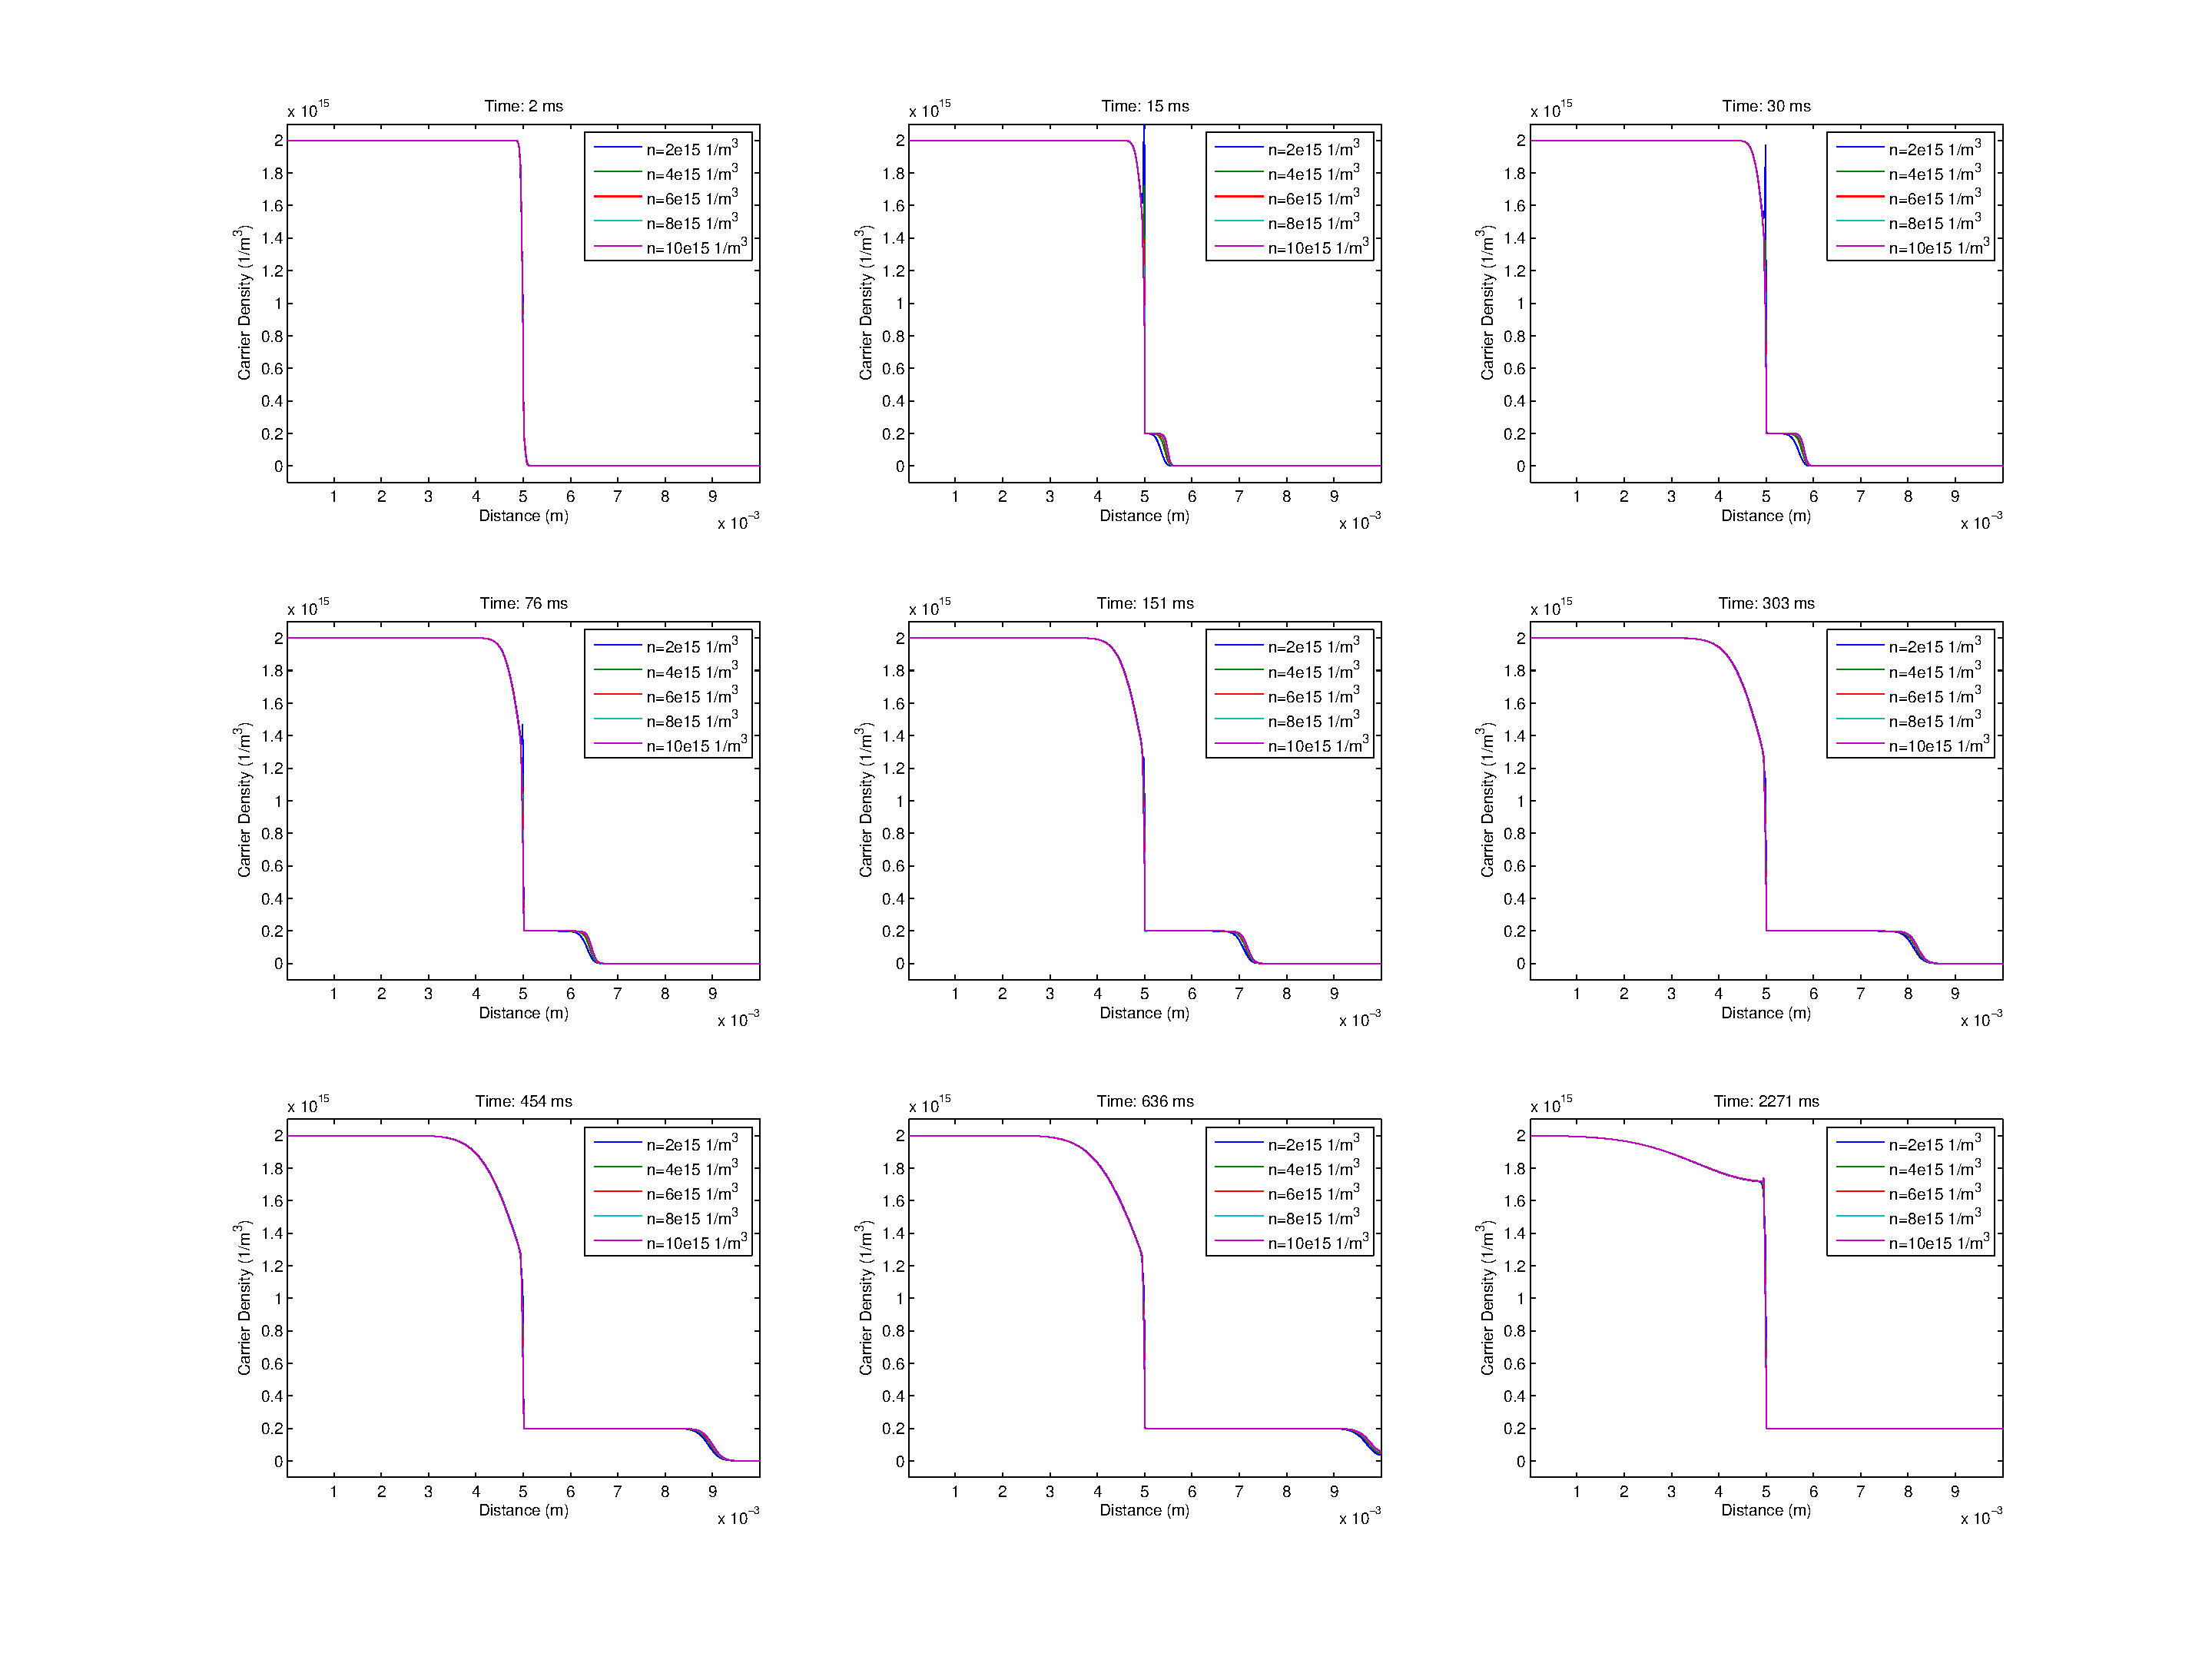
\includegraphics[scale=0.40]{Ex4Np_Time}
\caption{} 
\label{}
\end{figure}
\end{landscape}

\begin{landscape}
\begin{figure}[!htp]
\centering
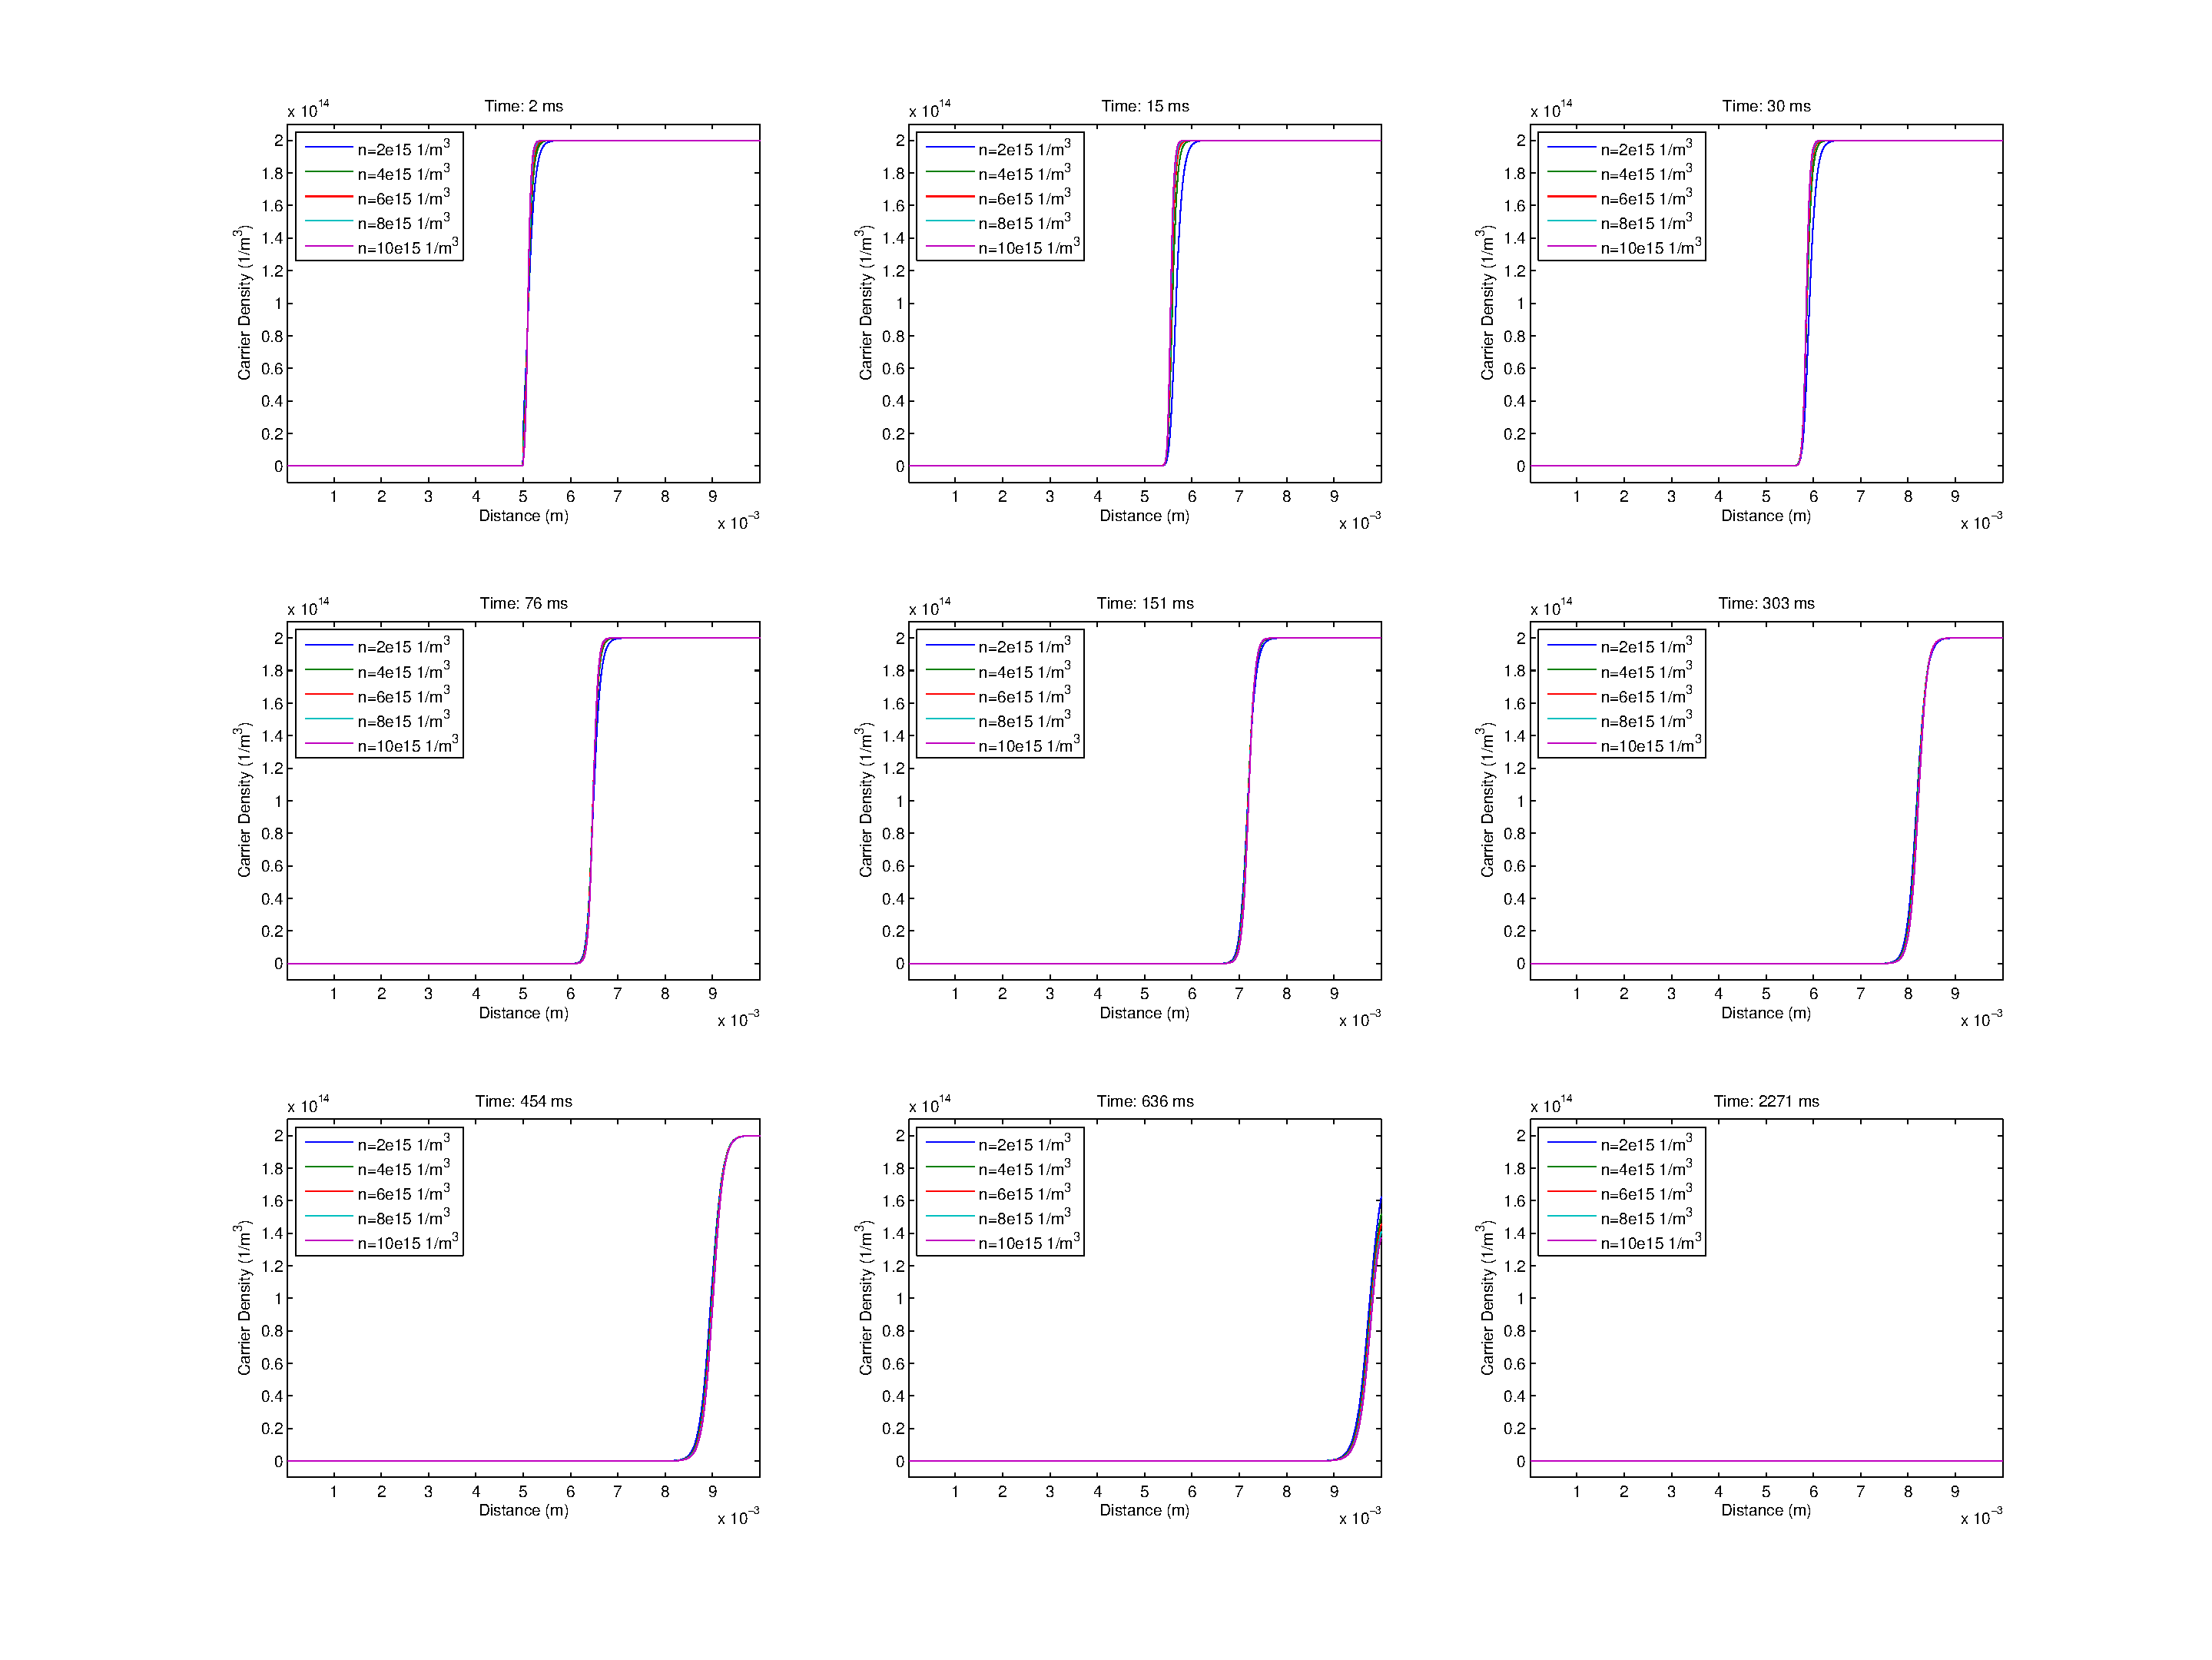
\includegraphics[scale=0.40]{Ex4p_Time}
\caption{} 
\label{}
\end{figure}
\end{landscape}

\begin{landscape}
\begin{figure}[!htp]
\centering
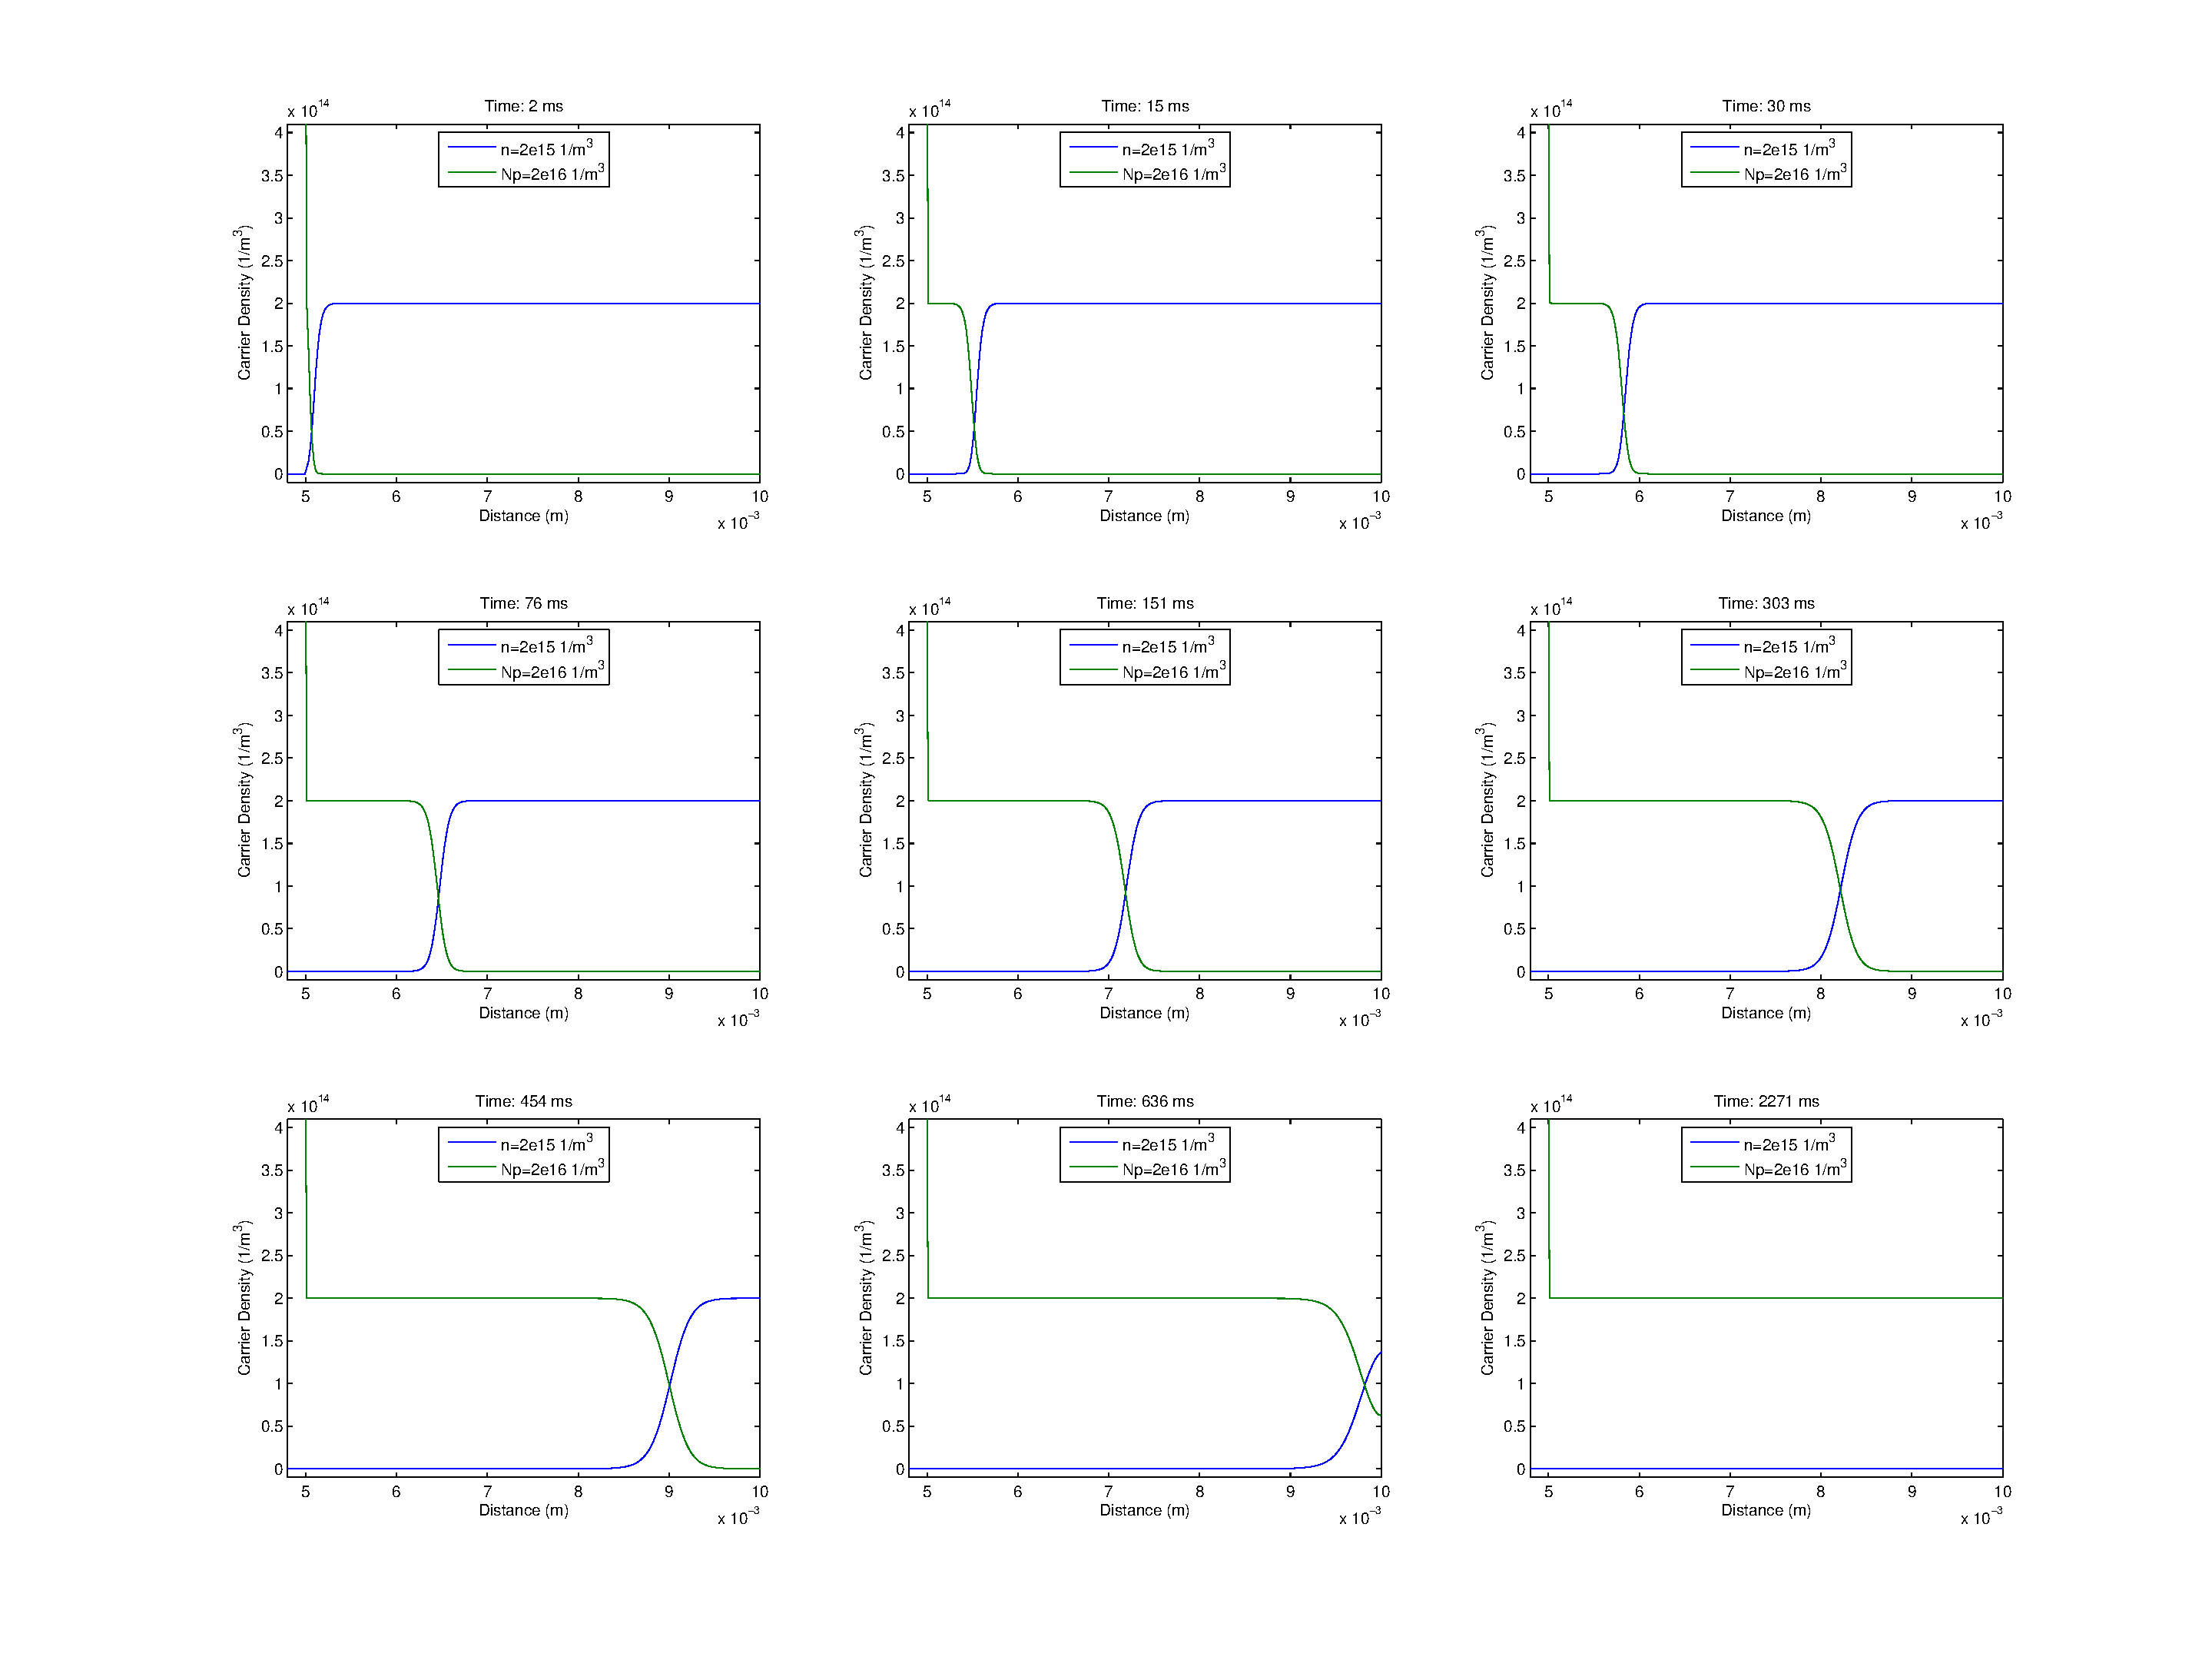
\includegraphics[scale=0.40]{Ex4pNp_Time}
\caption{} 
\label{}
\end{figure}
\end{landscape}

\begin{landscape}
\begin{figure}[!htp]
\centering
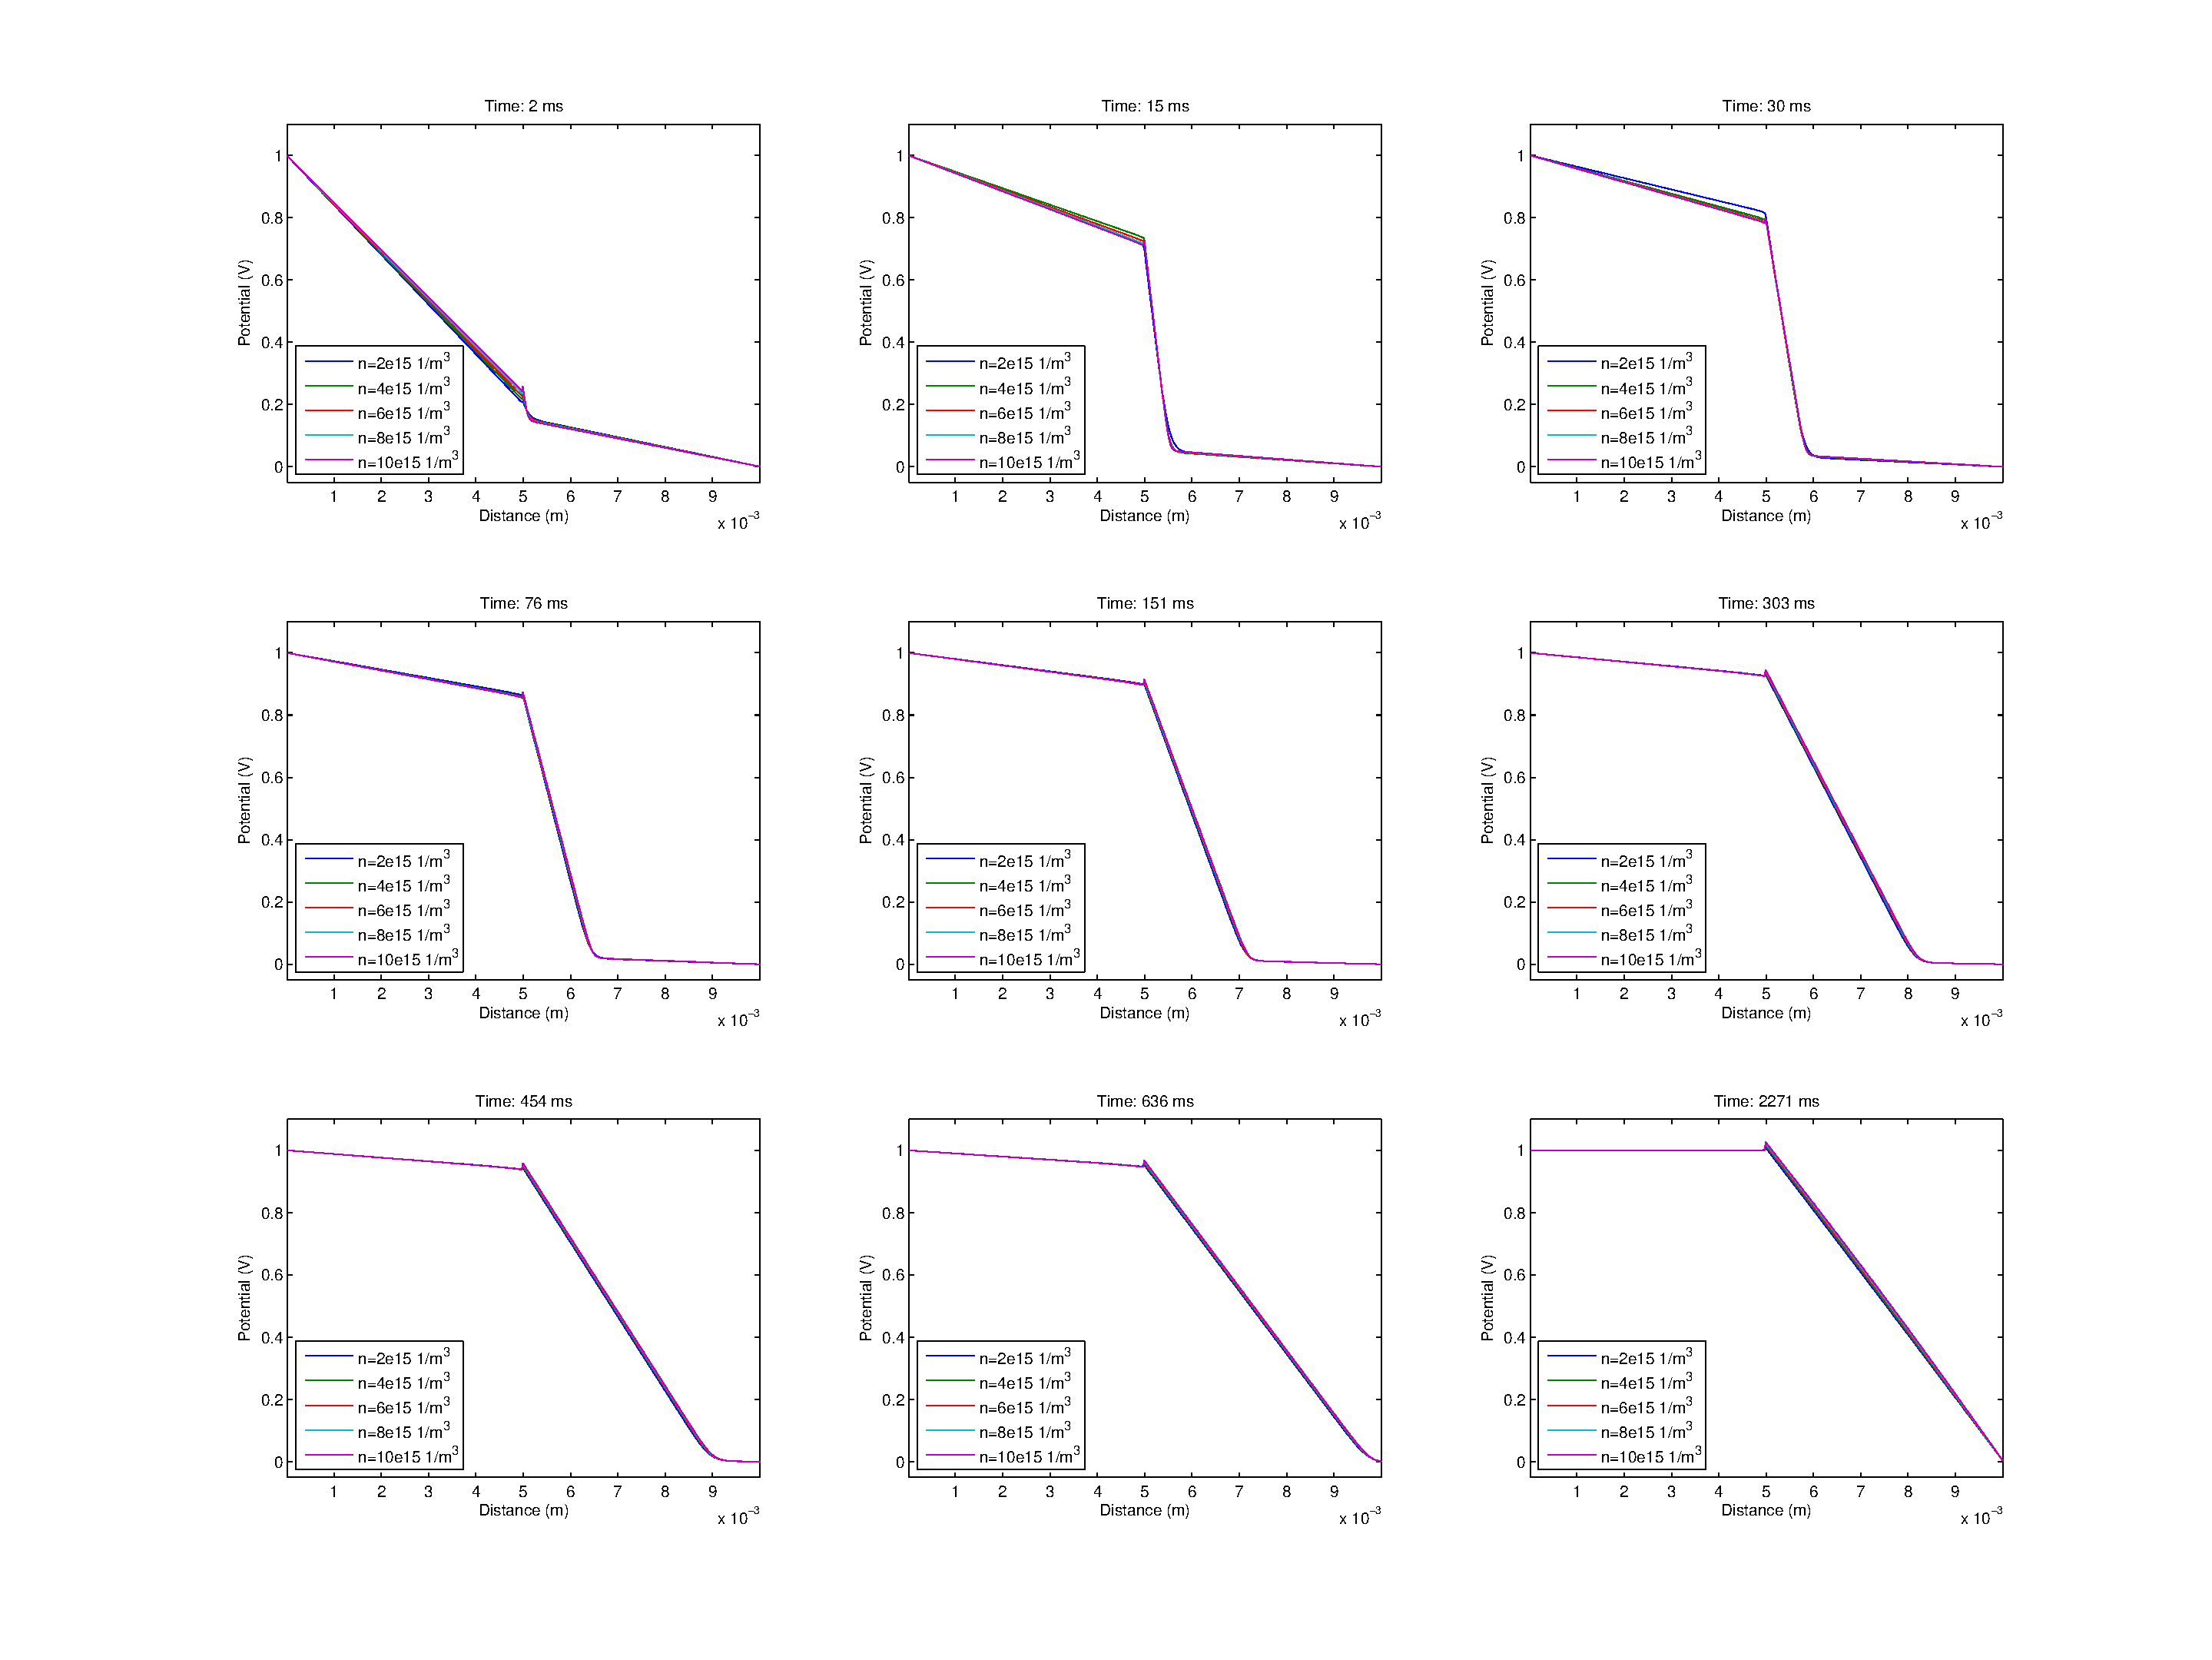
\includegraphics[scale=0.40]{Ex4V_Time}
\caption{} 
\label{}
\end{figure}
\end{landscape}

\section{Ion movement in a 1-D Memristor}


\begin{landscape}
\begin{figure}[!htp]
\centering
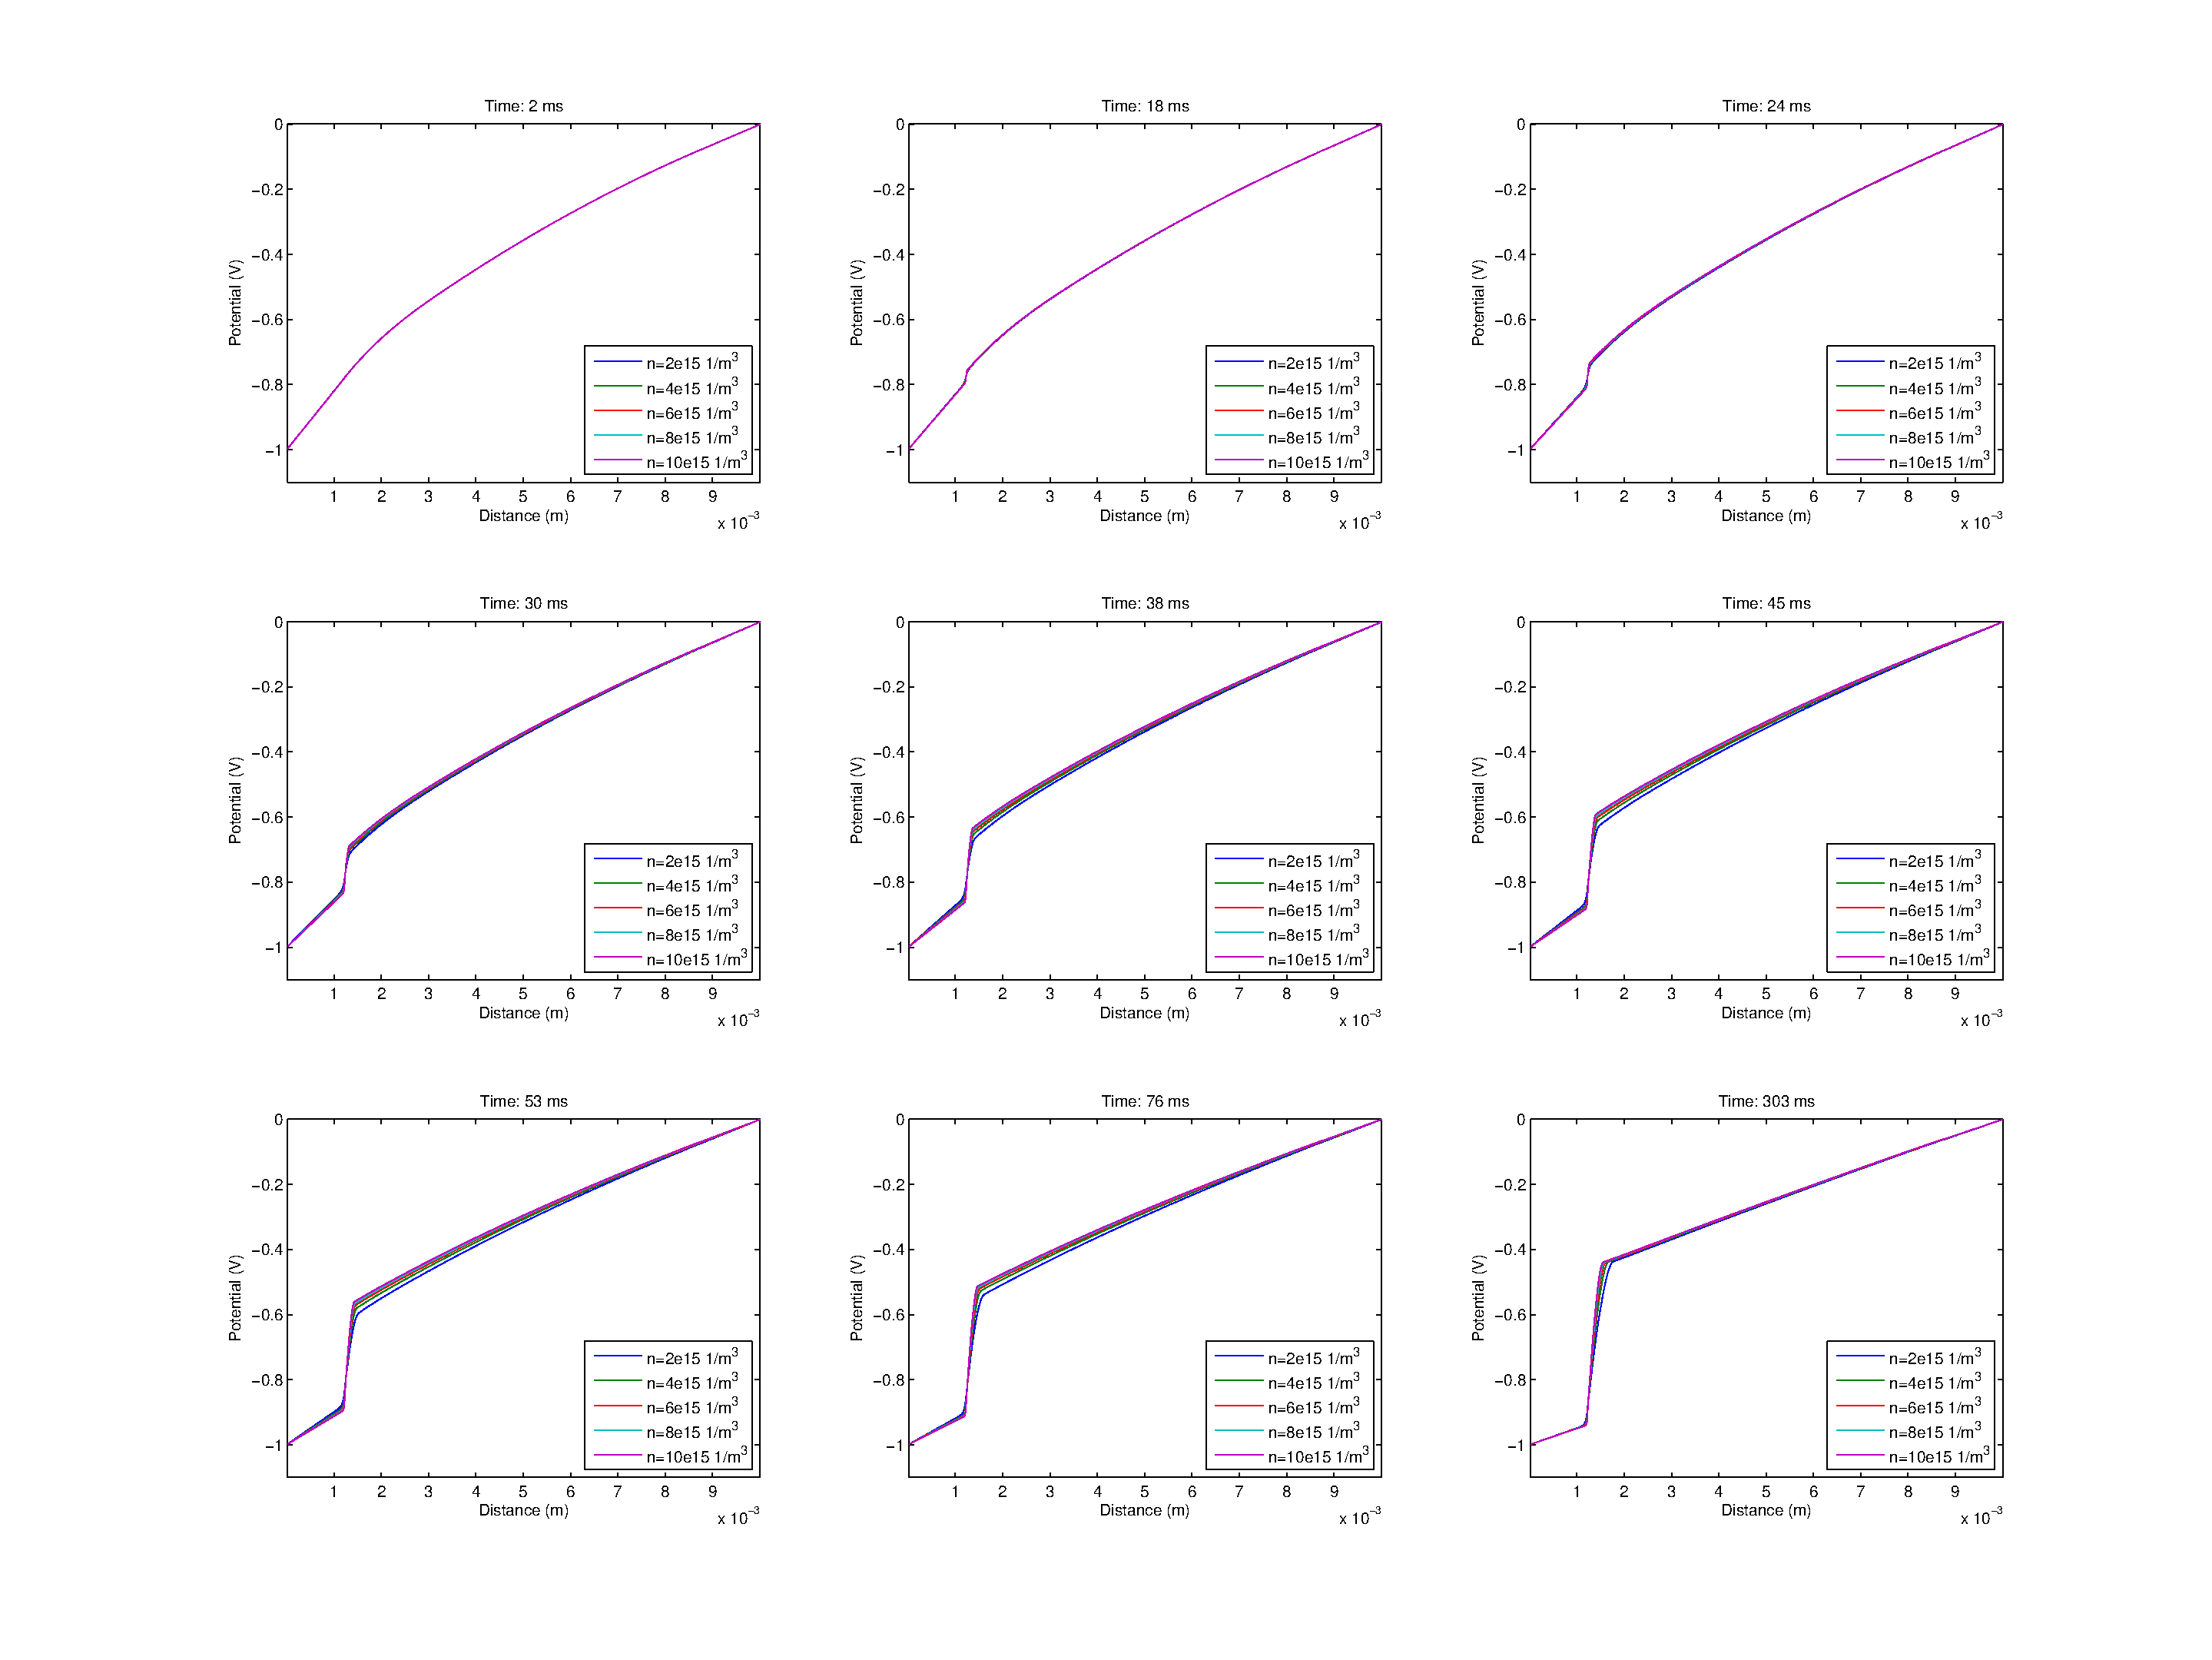
\includegraphics[scale=0.40]{Ex5V_Time1}
\caption{} 
\label{}
\end{figure}
\end{landscape}

\begin{landscape}
\begin{figure}[!htp]
\centering
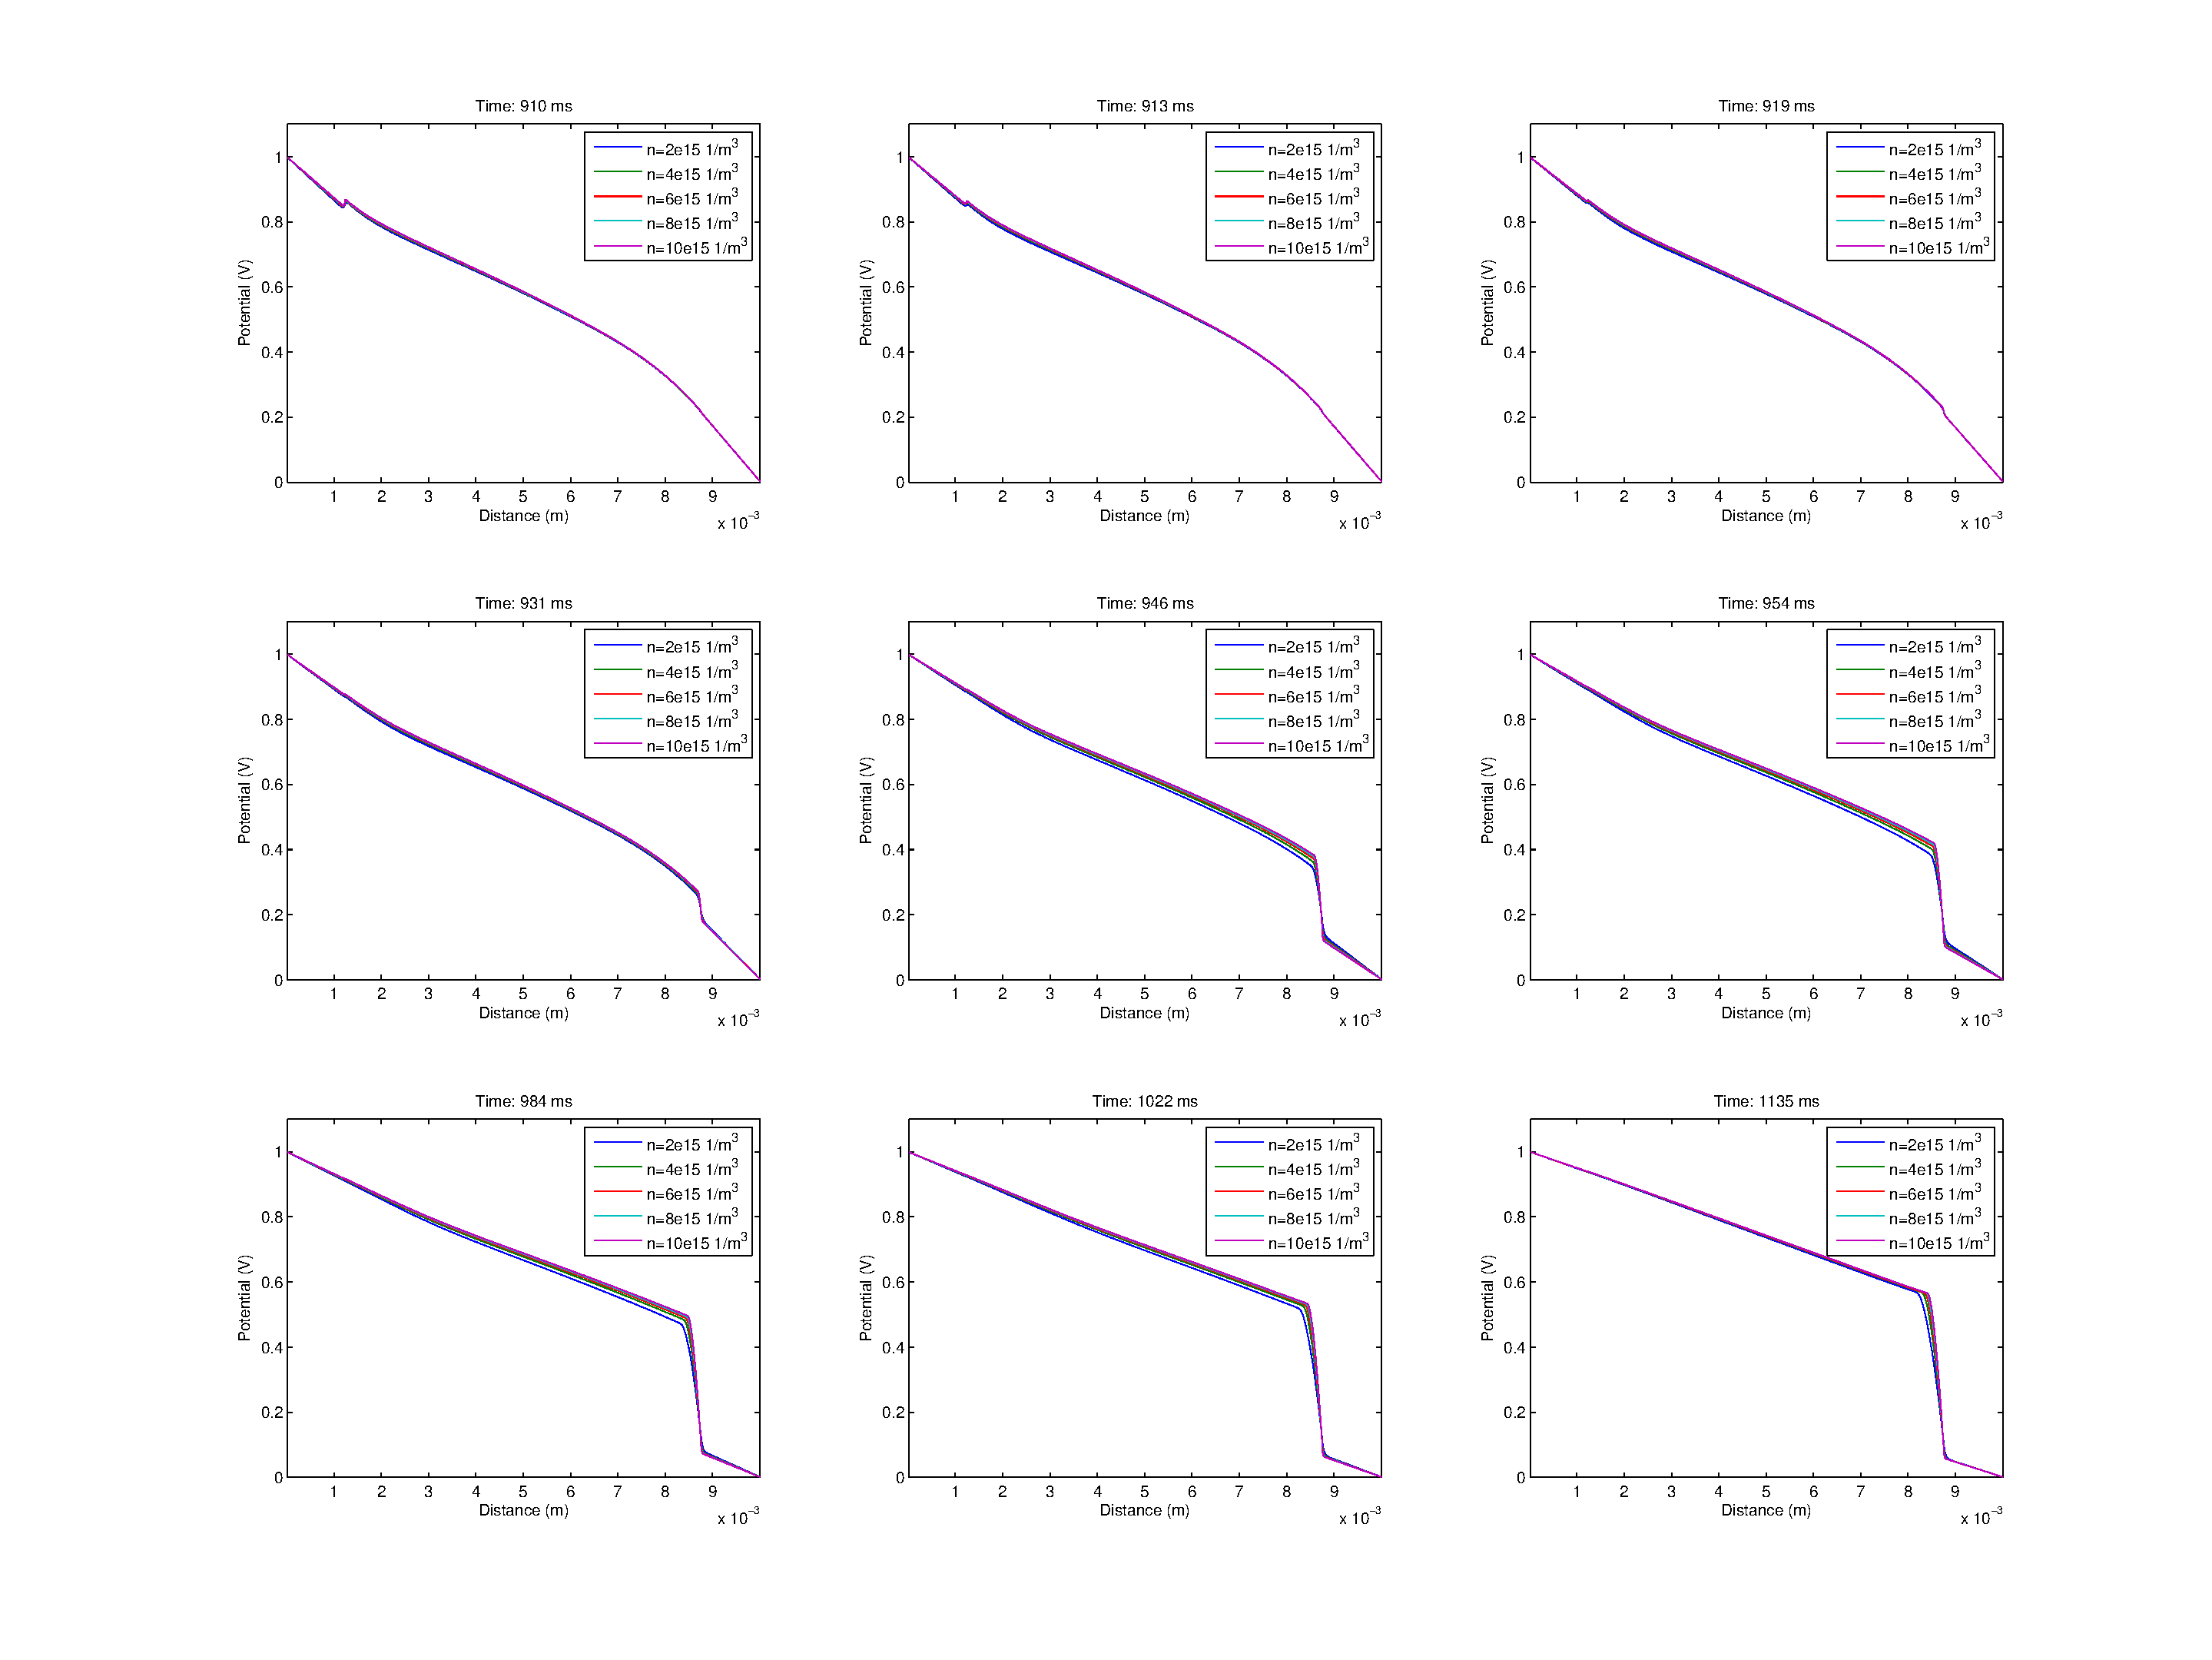
\includegraphics[scale=0.40]{Ex5V_Time2}
\caption{} 
\label{}
\end{figure}
\end{landscape}

\begin{landscape}
\begin{figure}[!htp]
\centering
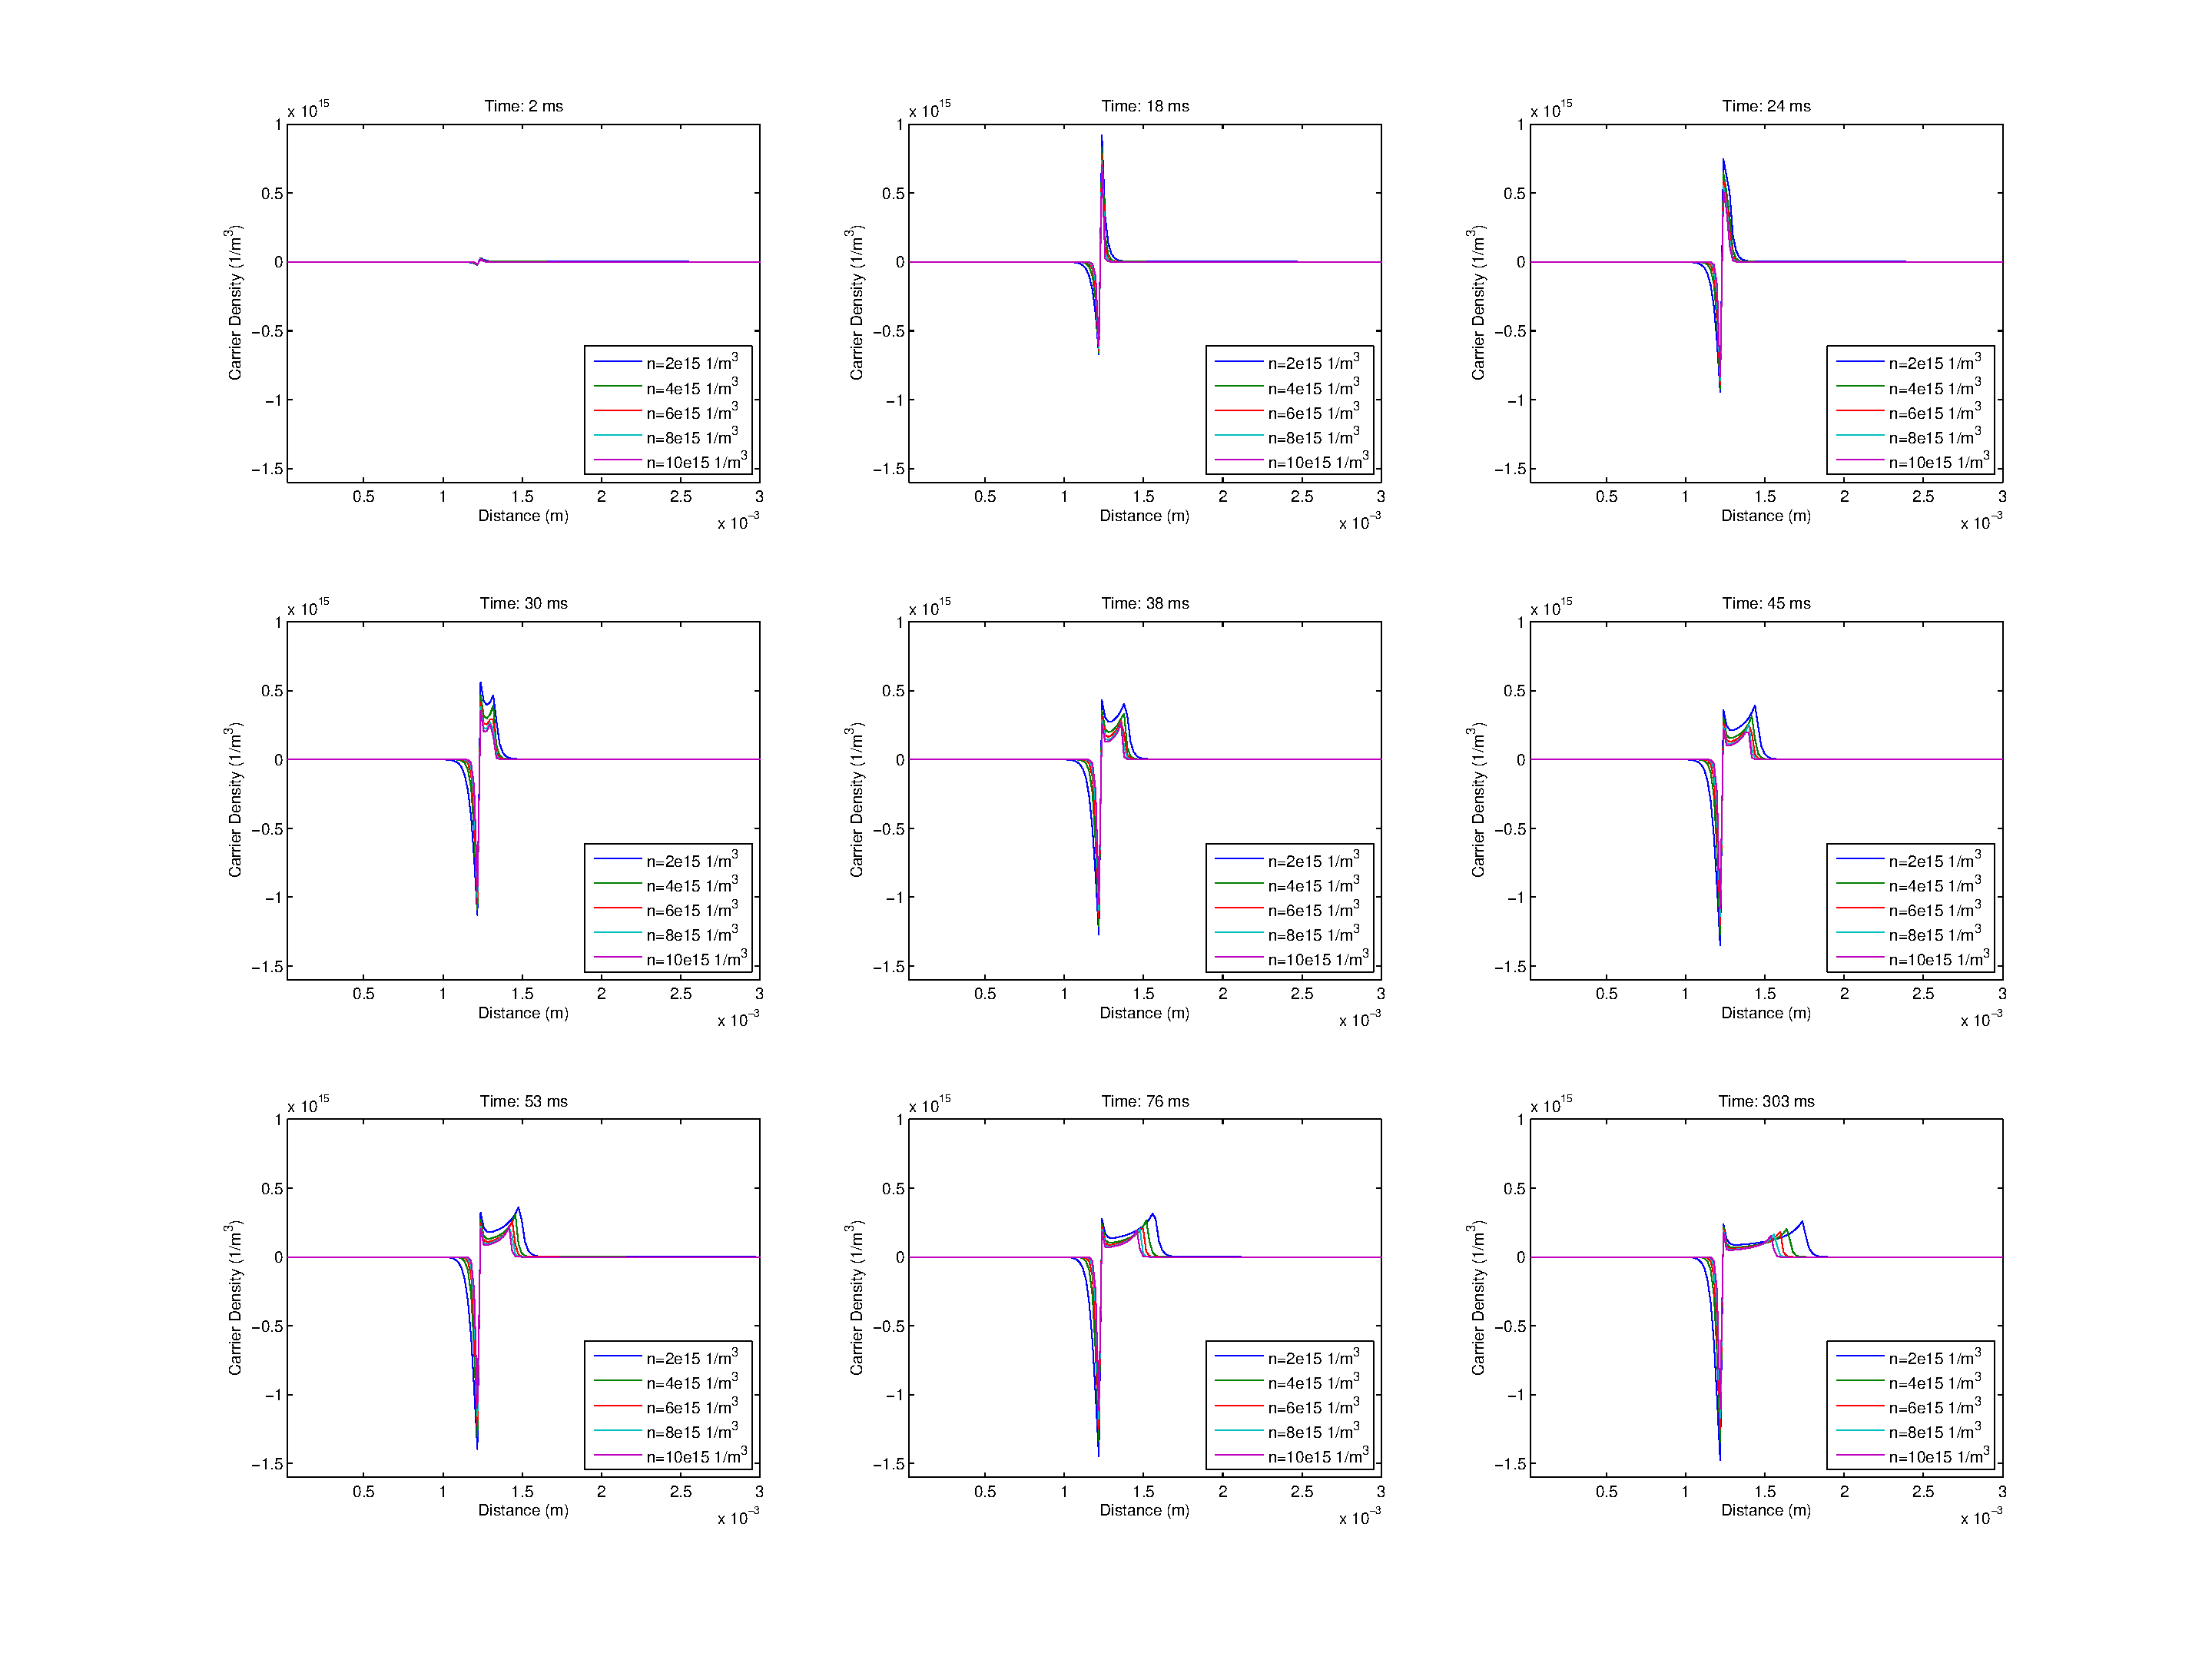
\includegraphics[scale=0.40]{Ex5NetQ_Time1}
\caption{} 
\label{}
\end{figure}
\end{landscape}

\begin{landscape}
\begin{figure}[!htp]
\centering
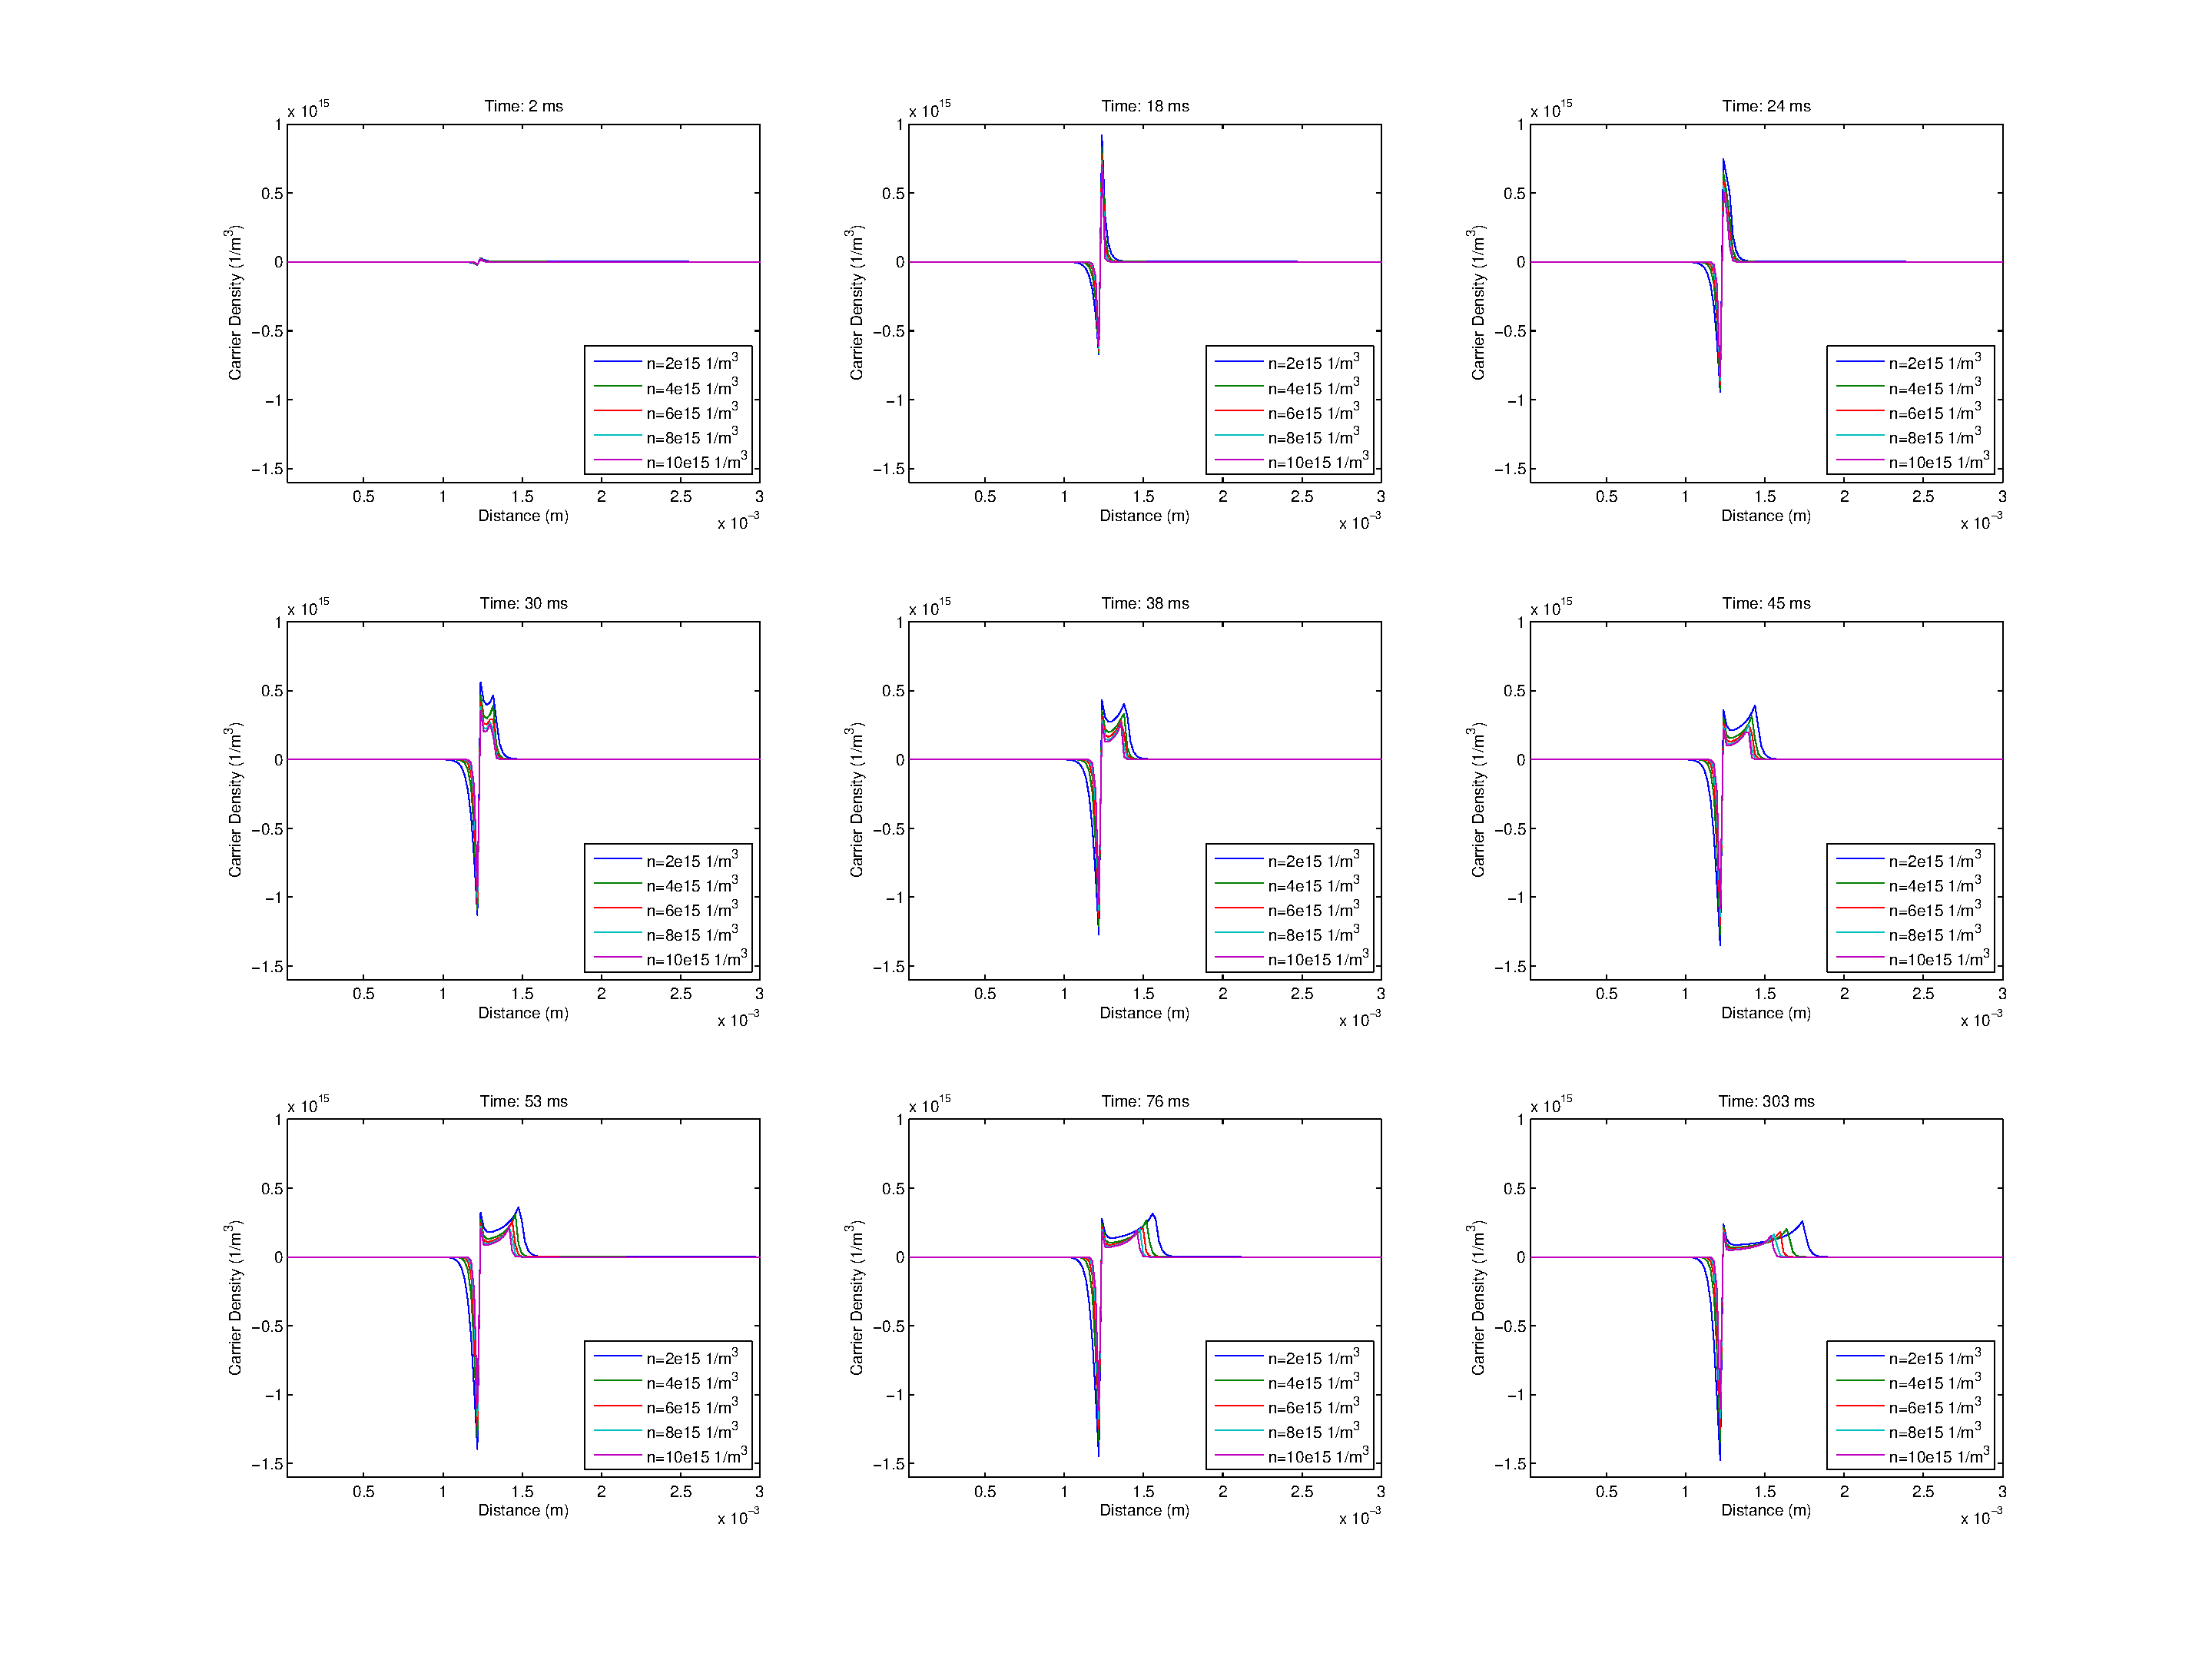
\includegraphics[scale=0.40]{Ex5NetQ_Time1}
\caption{} 
\label{}
\end{figure}
\end{landscape}

\begin{landscape}
\begin{figure}[!htp]
\centering
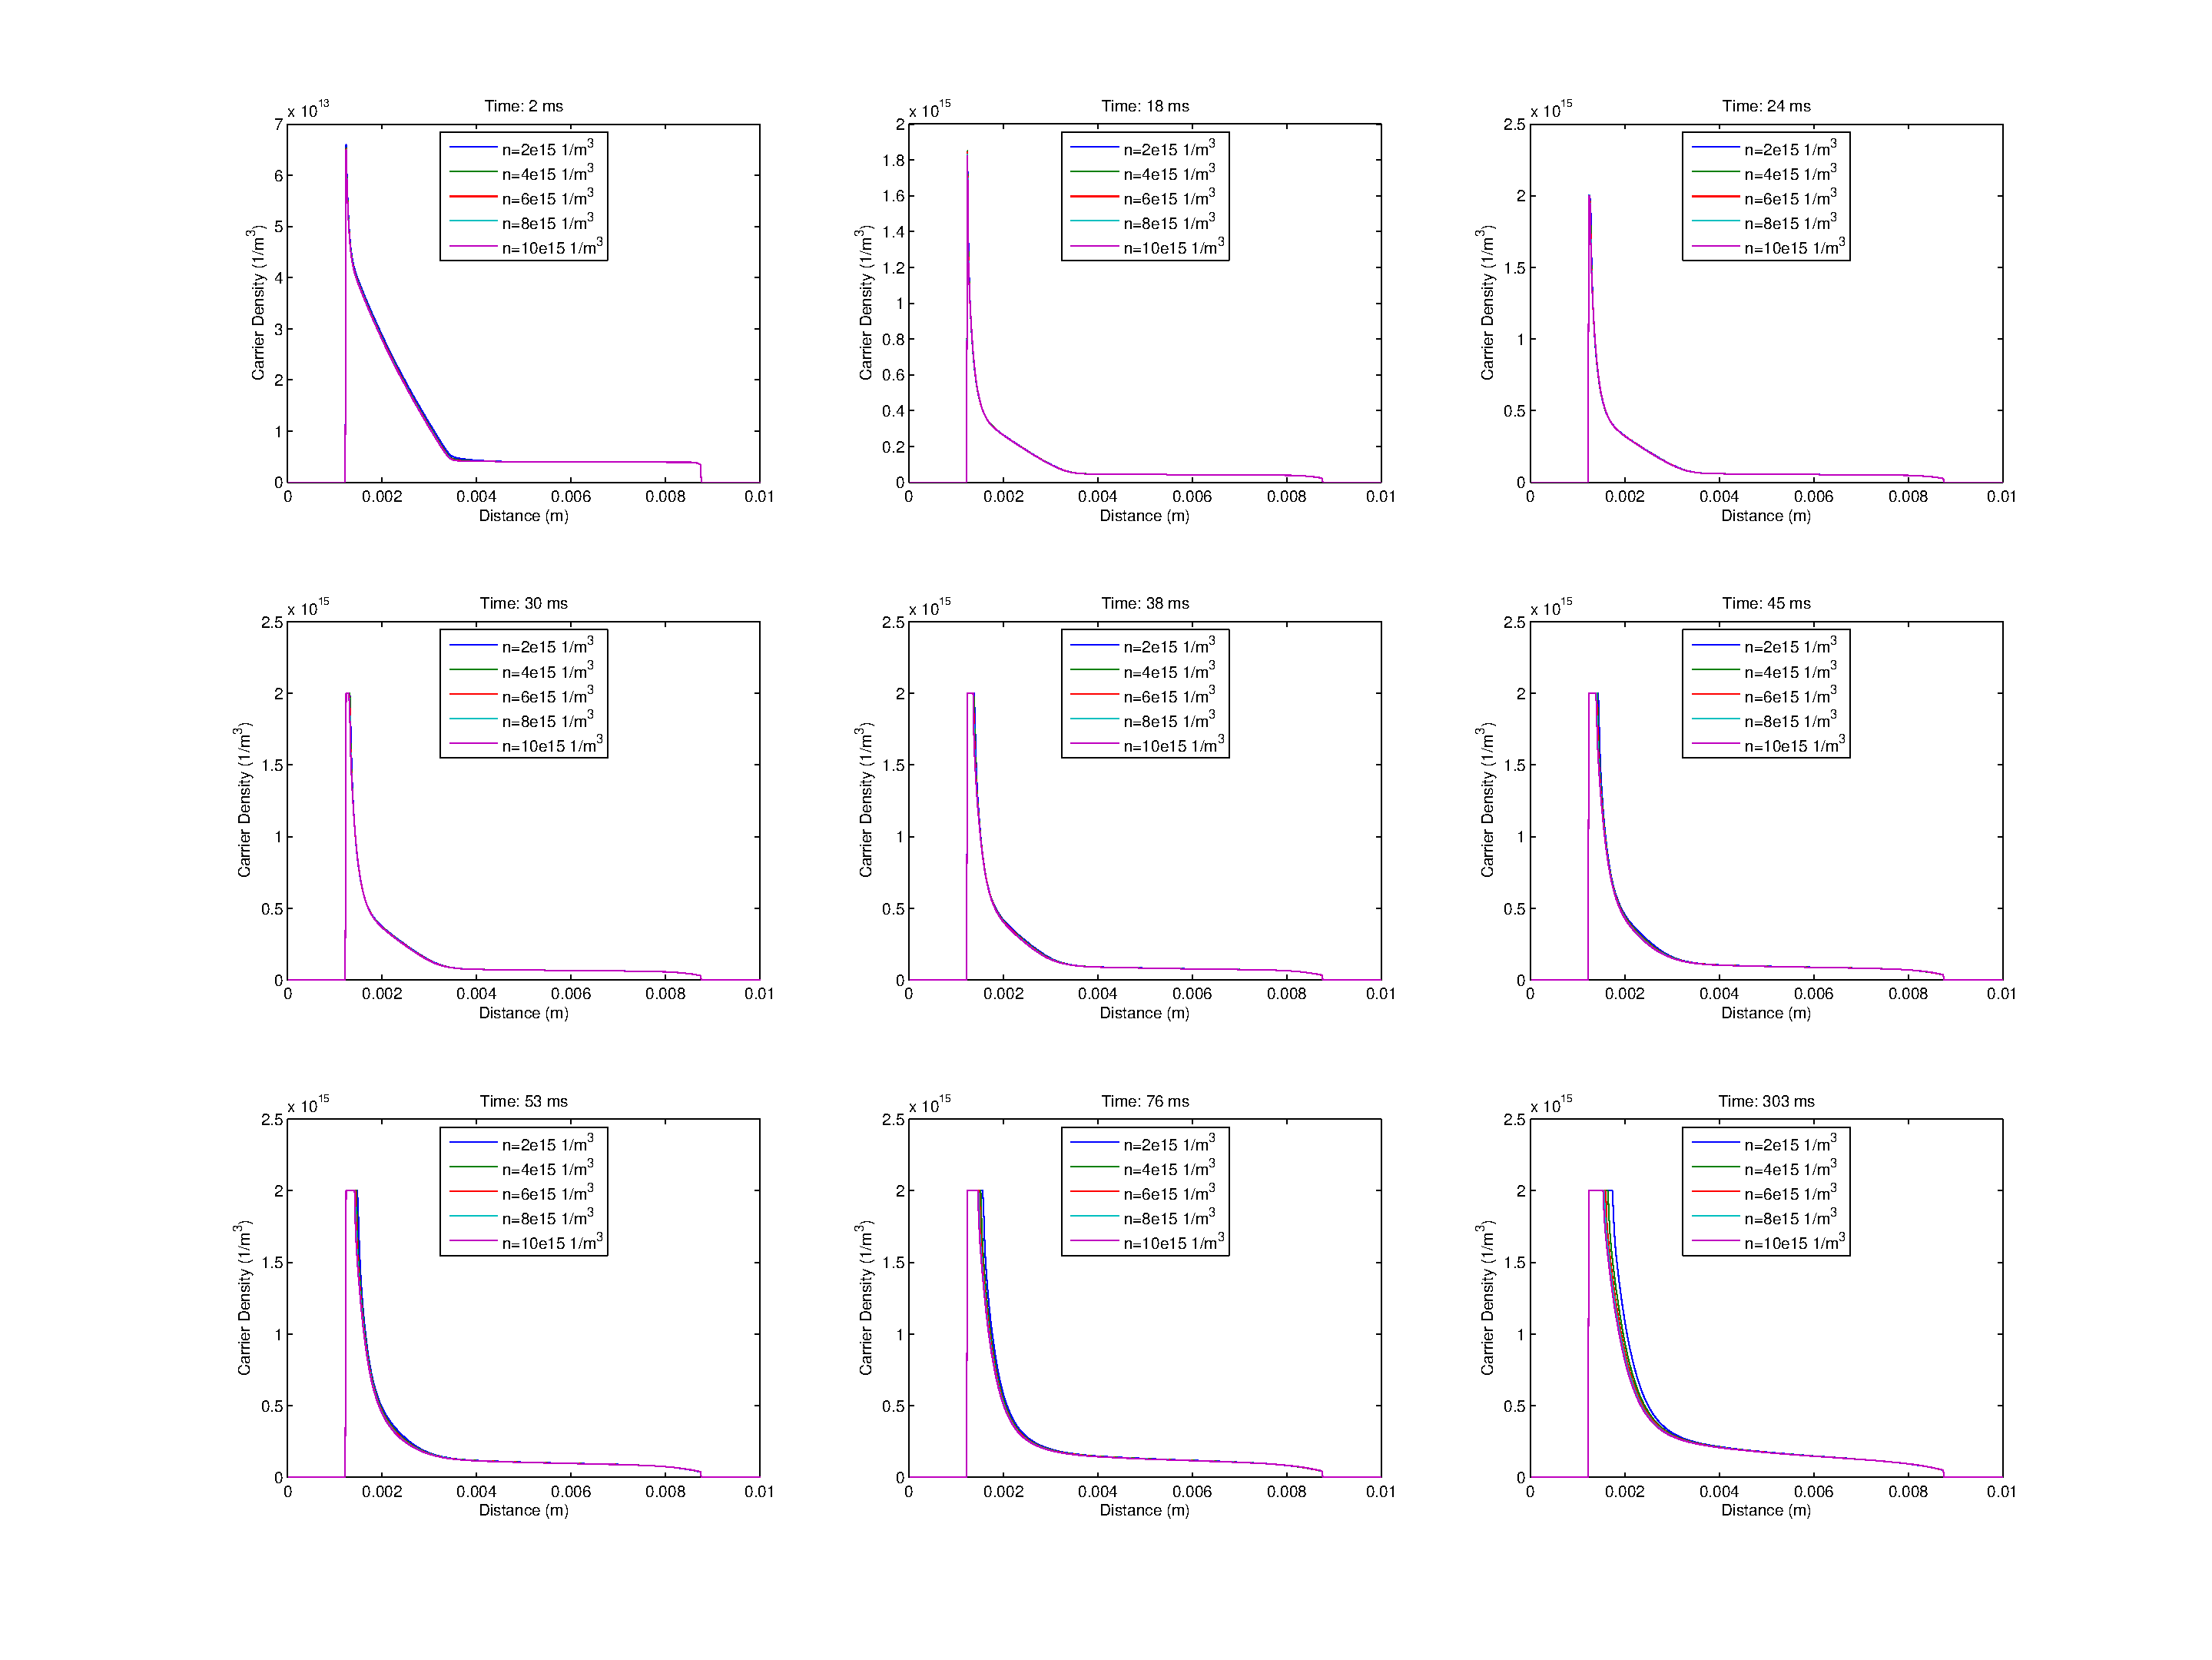
\includegraphics[scale=0.40]{Ex5Np_Time1}
\caption{} 
\label{}
\end{figure}
\end{landscape}

\begin{landscape}
\begin{figure}[!htp]
\centering
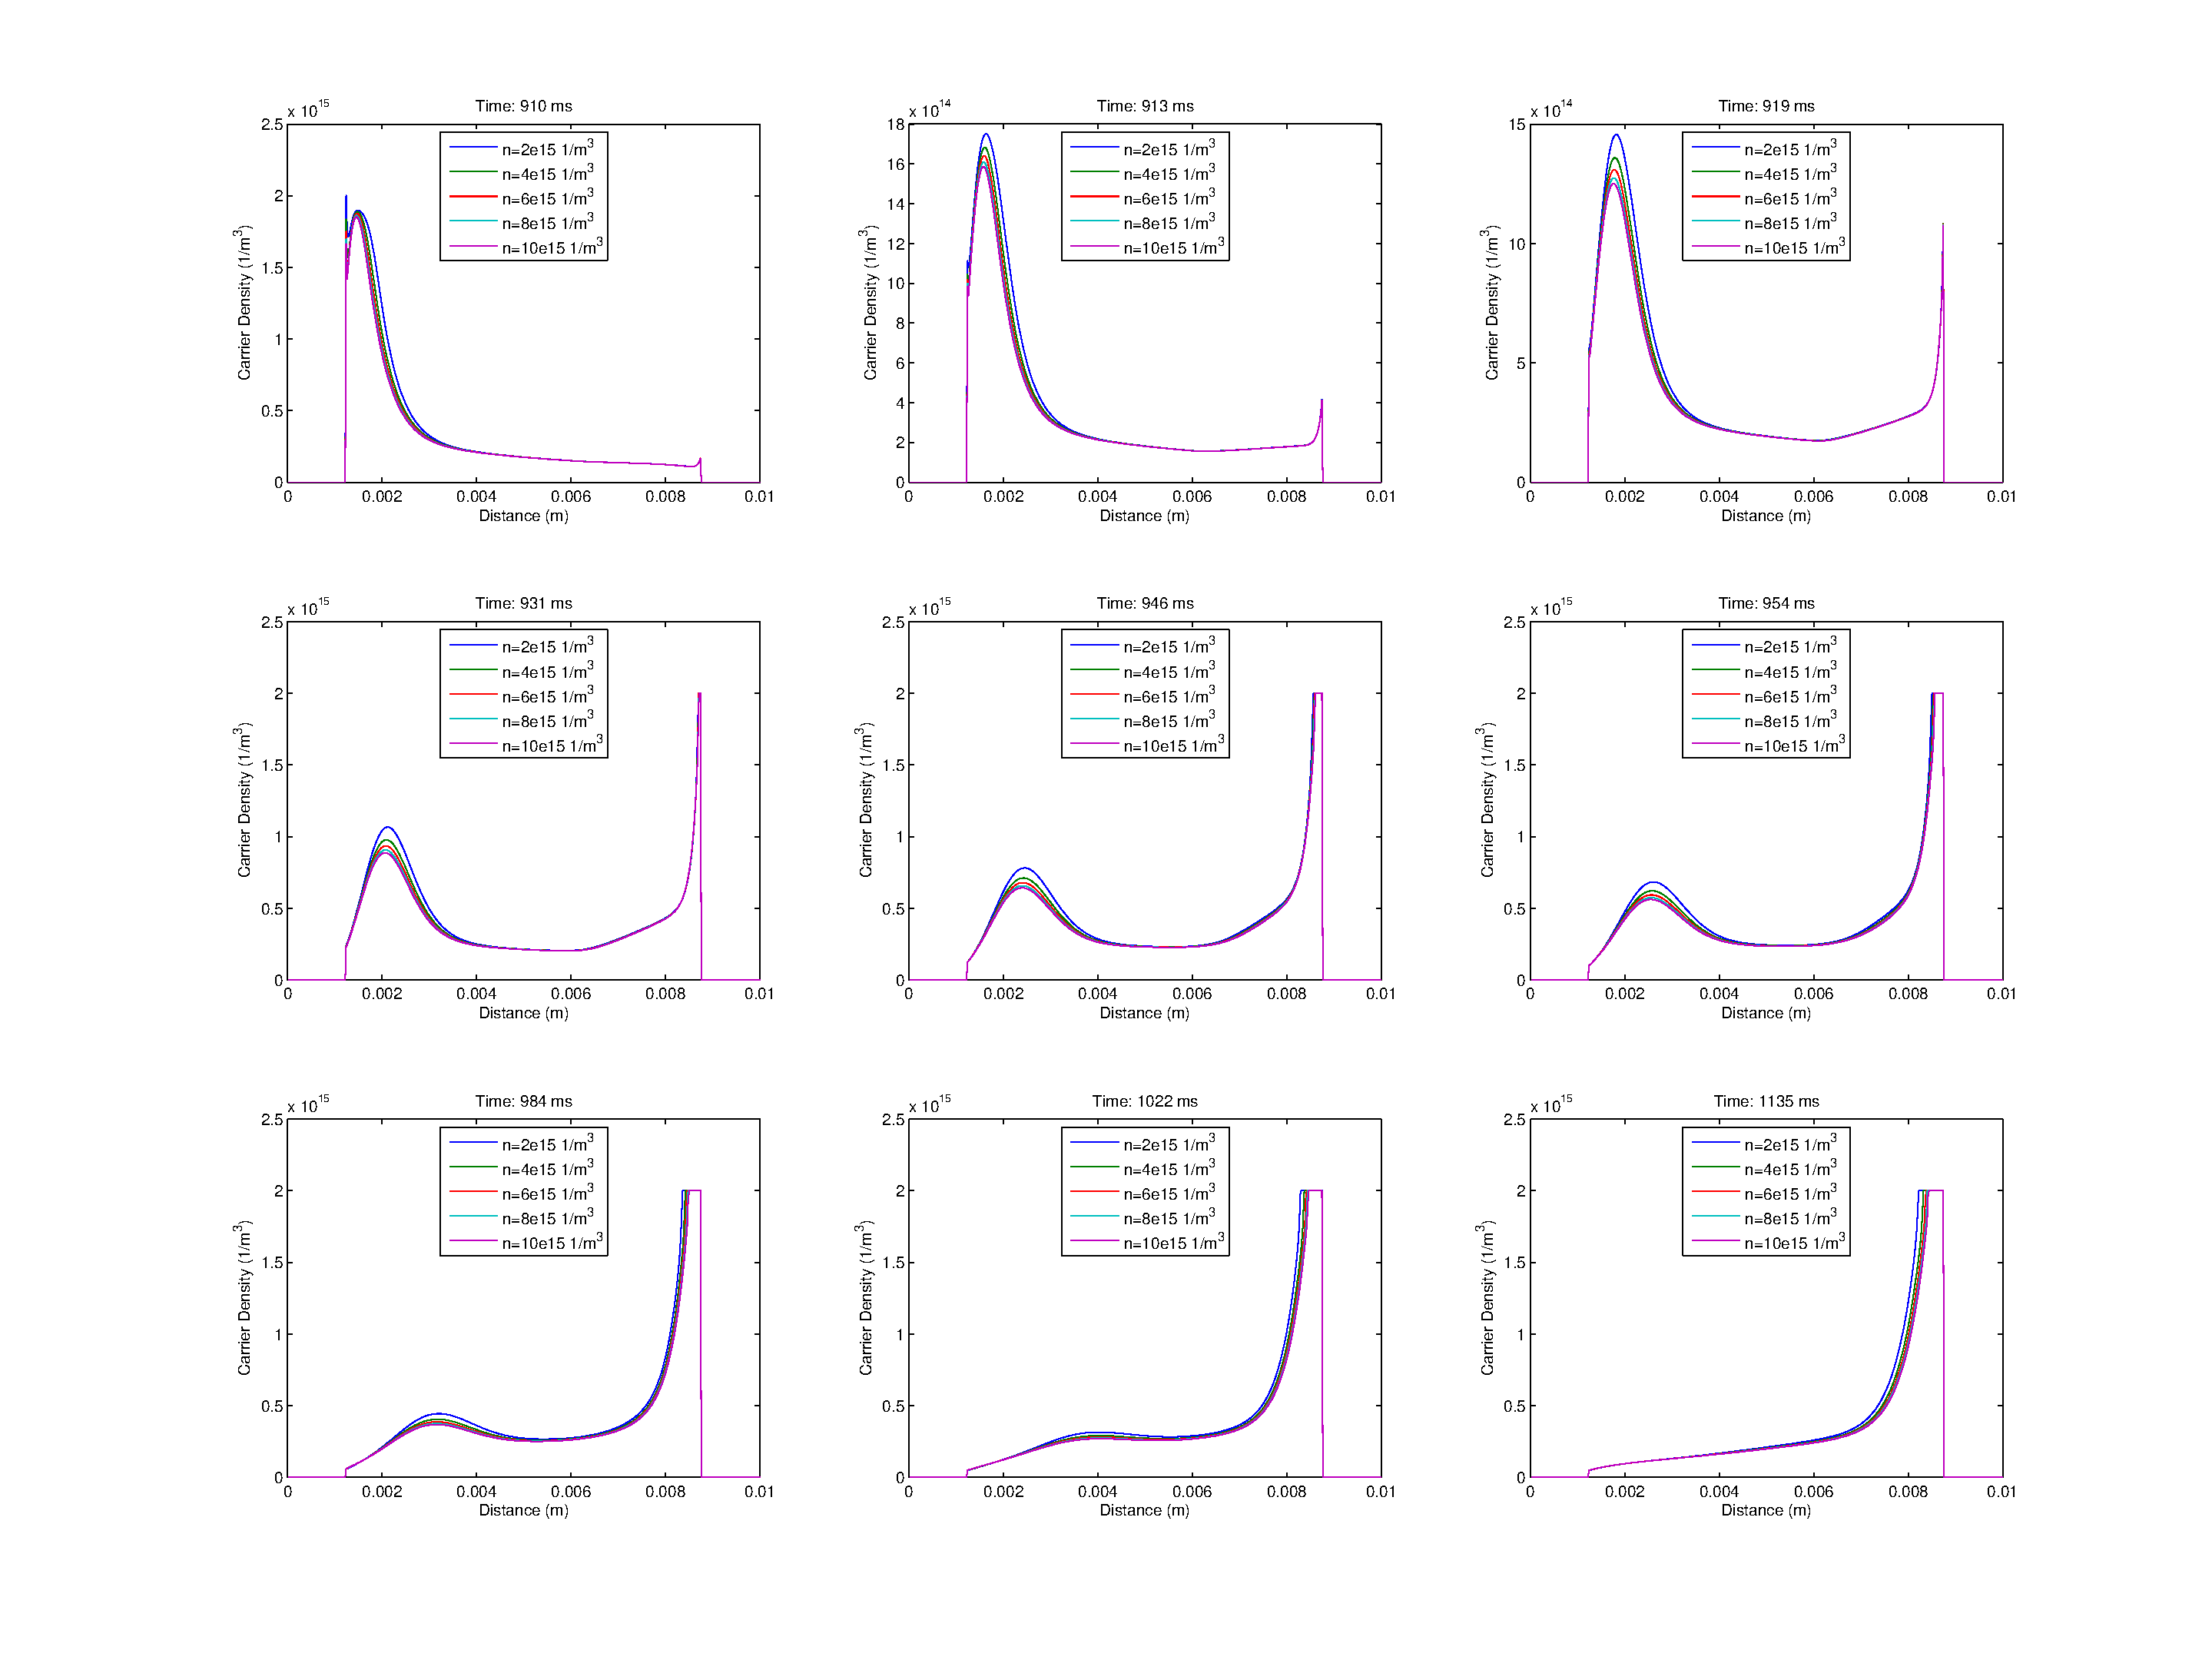
\includegraphics[scale=0.40]{Ex5Np_Time2}
\caption{} 
\label{}
\end{figure}
\end{landscape}

\begin{landscape}
\begin{figure}[!htp]
\centering
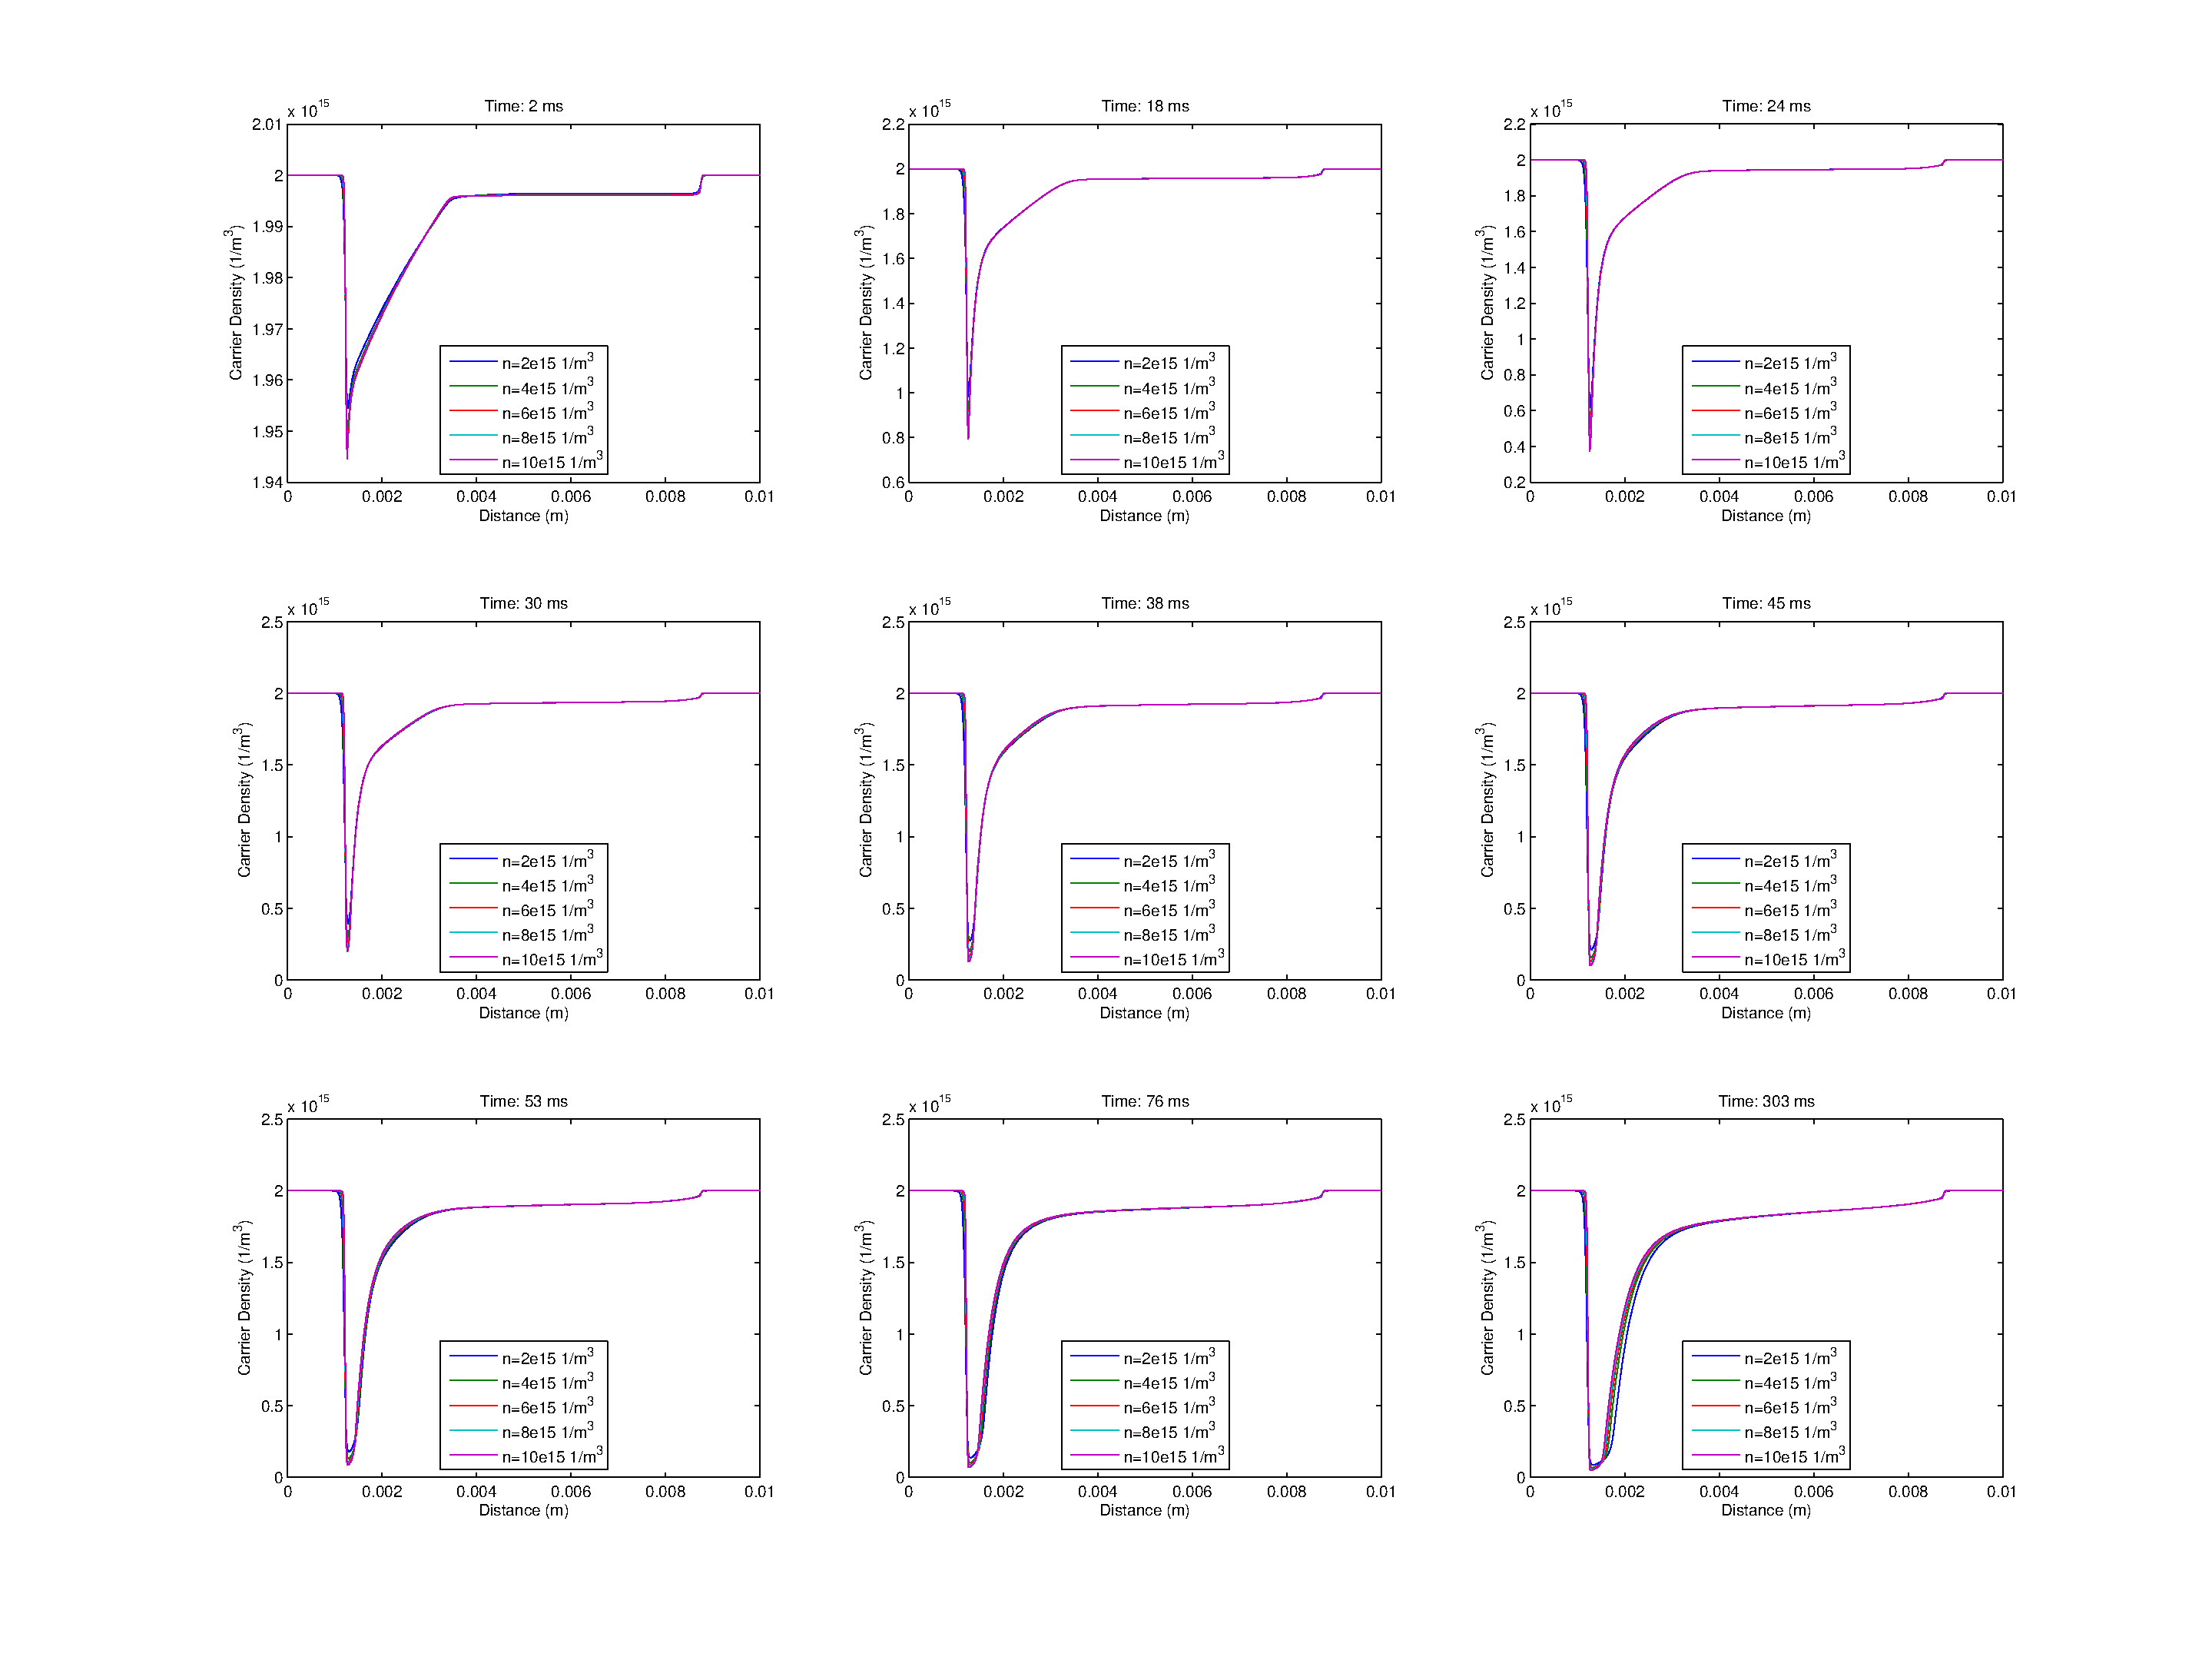
\includegraphics[scale=0.40]{Ex5p_Time1}
\caption{} 
\label{}
\end{figure}
\end{landscape}

\begin{landscape}
\begin{figure}[!htp]
\centering
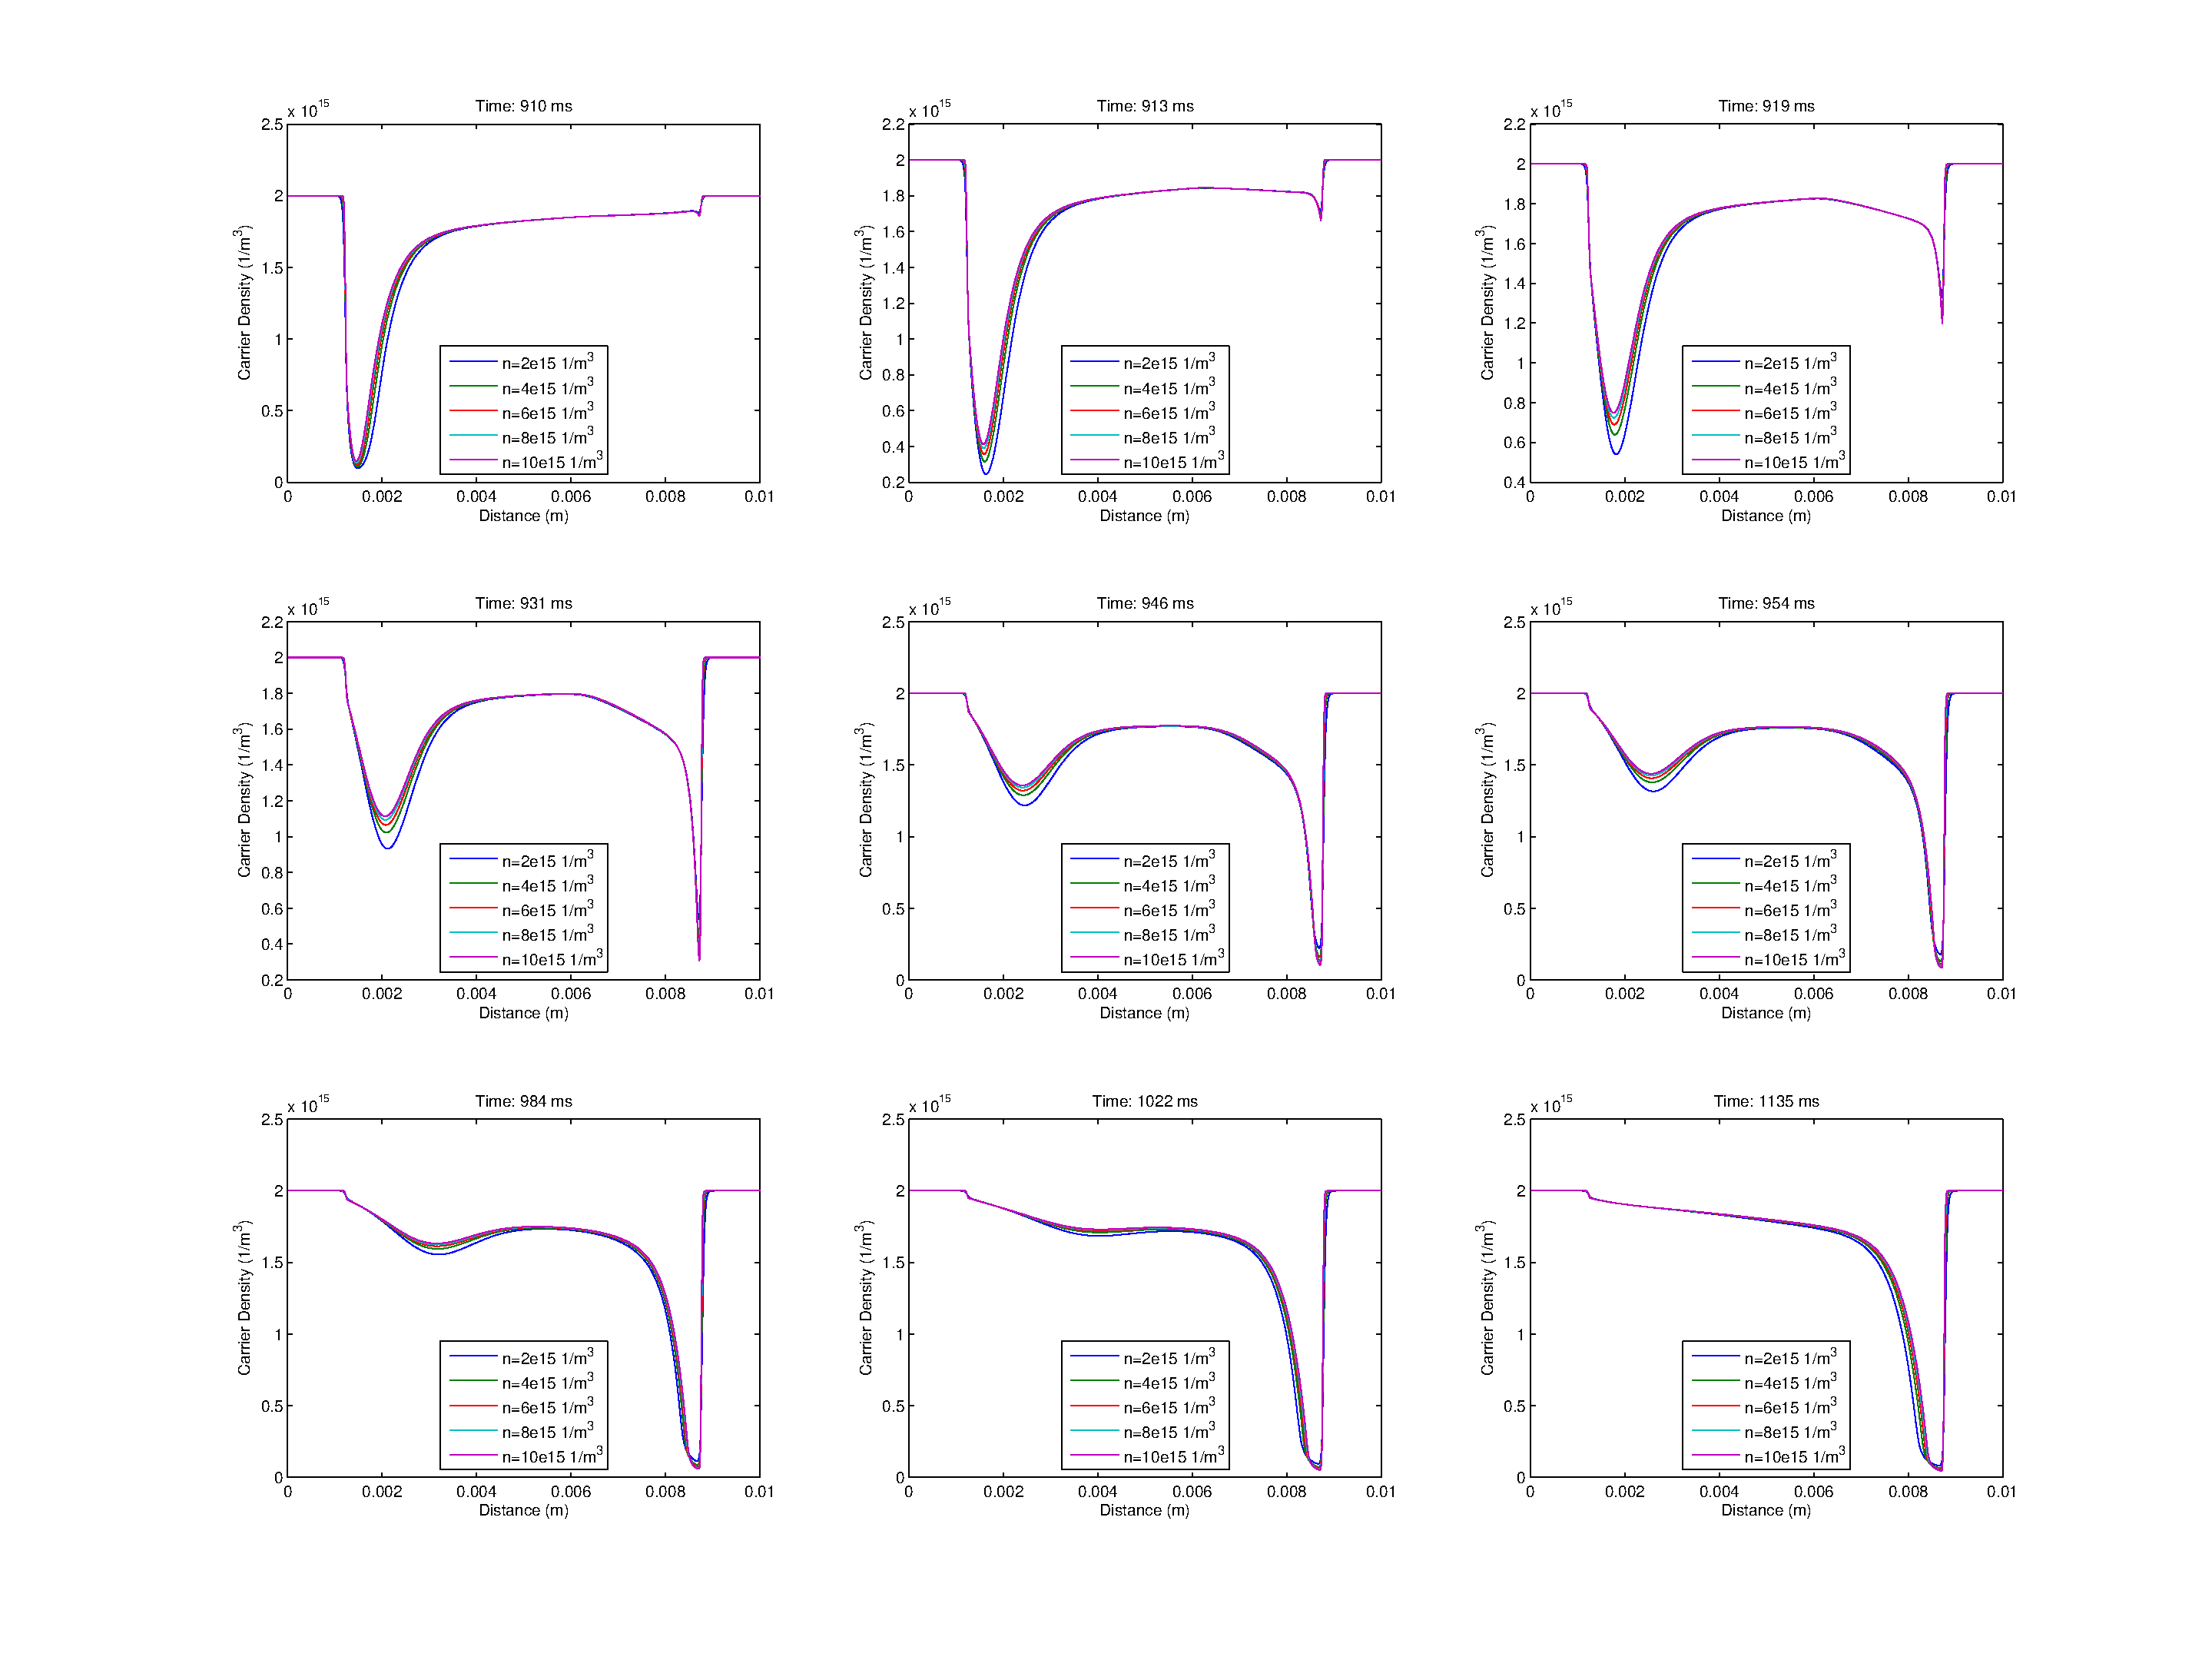
\includegraphics[scale=0.40]{Ex5p_Time2}
\caption{} 
\label{}
\end{figure}
\end{landscape}


\begin{landscape}
\begin{figure}[!htp]
\centering
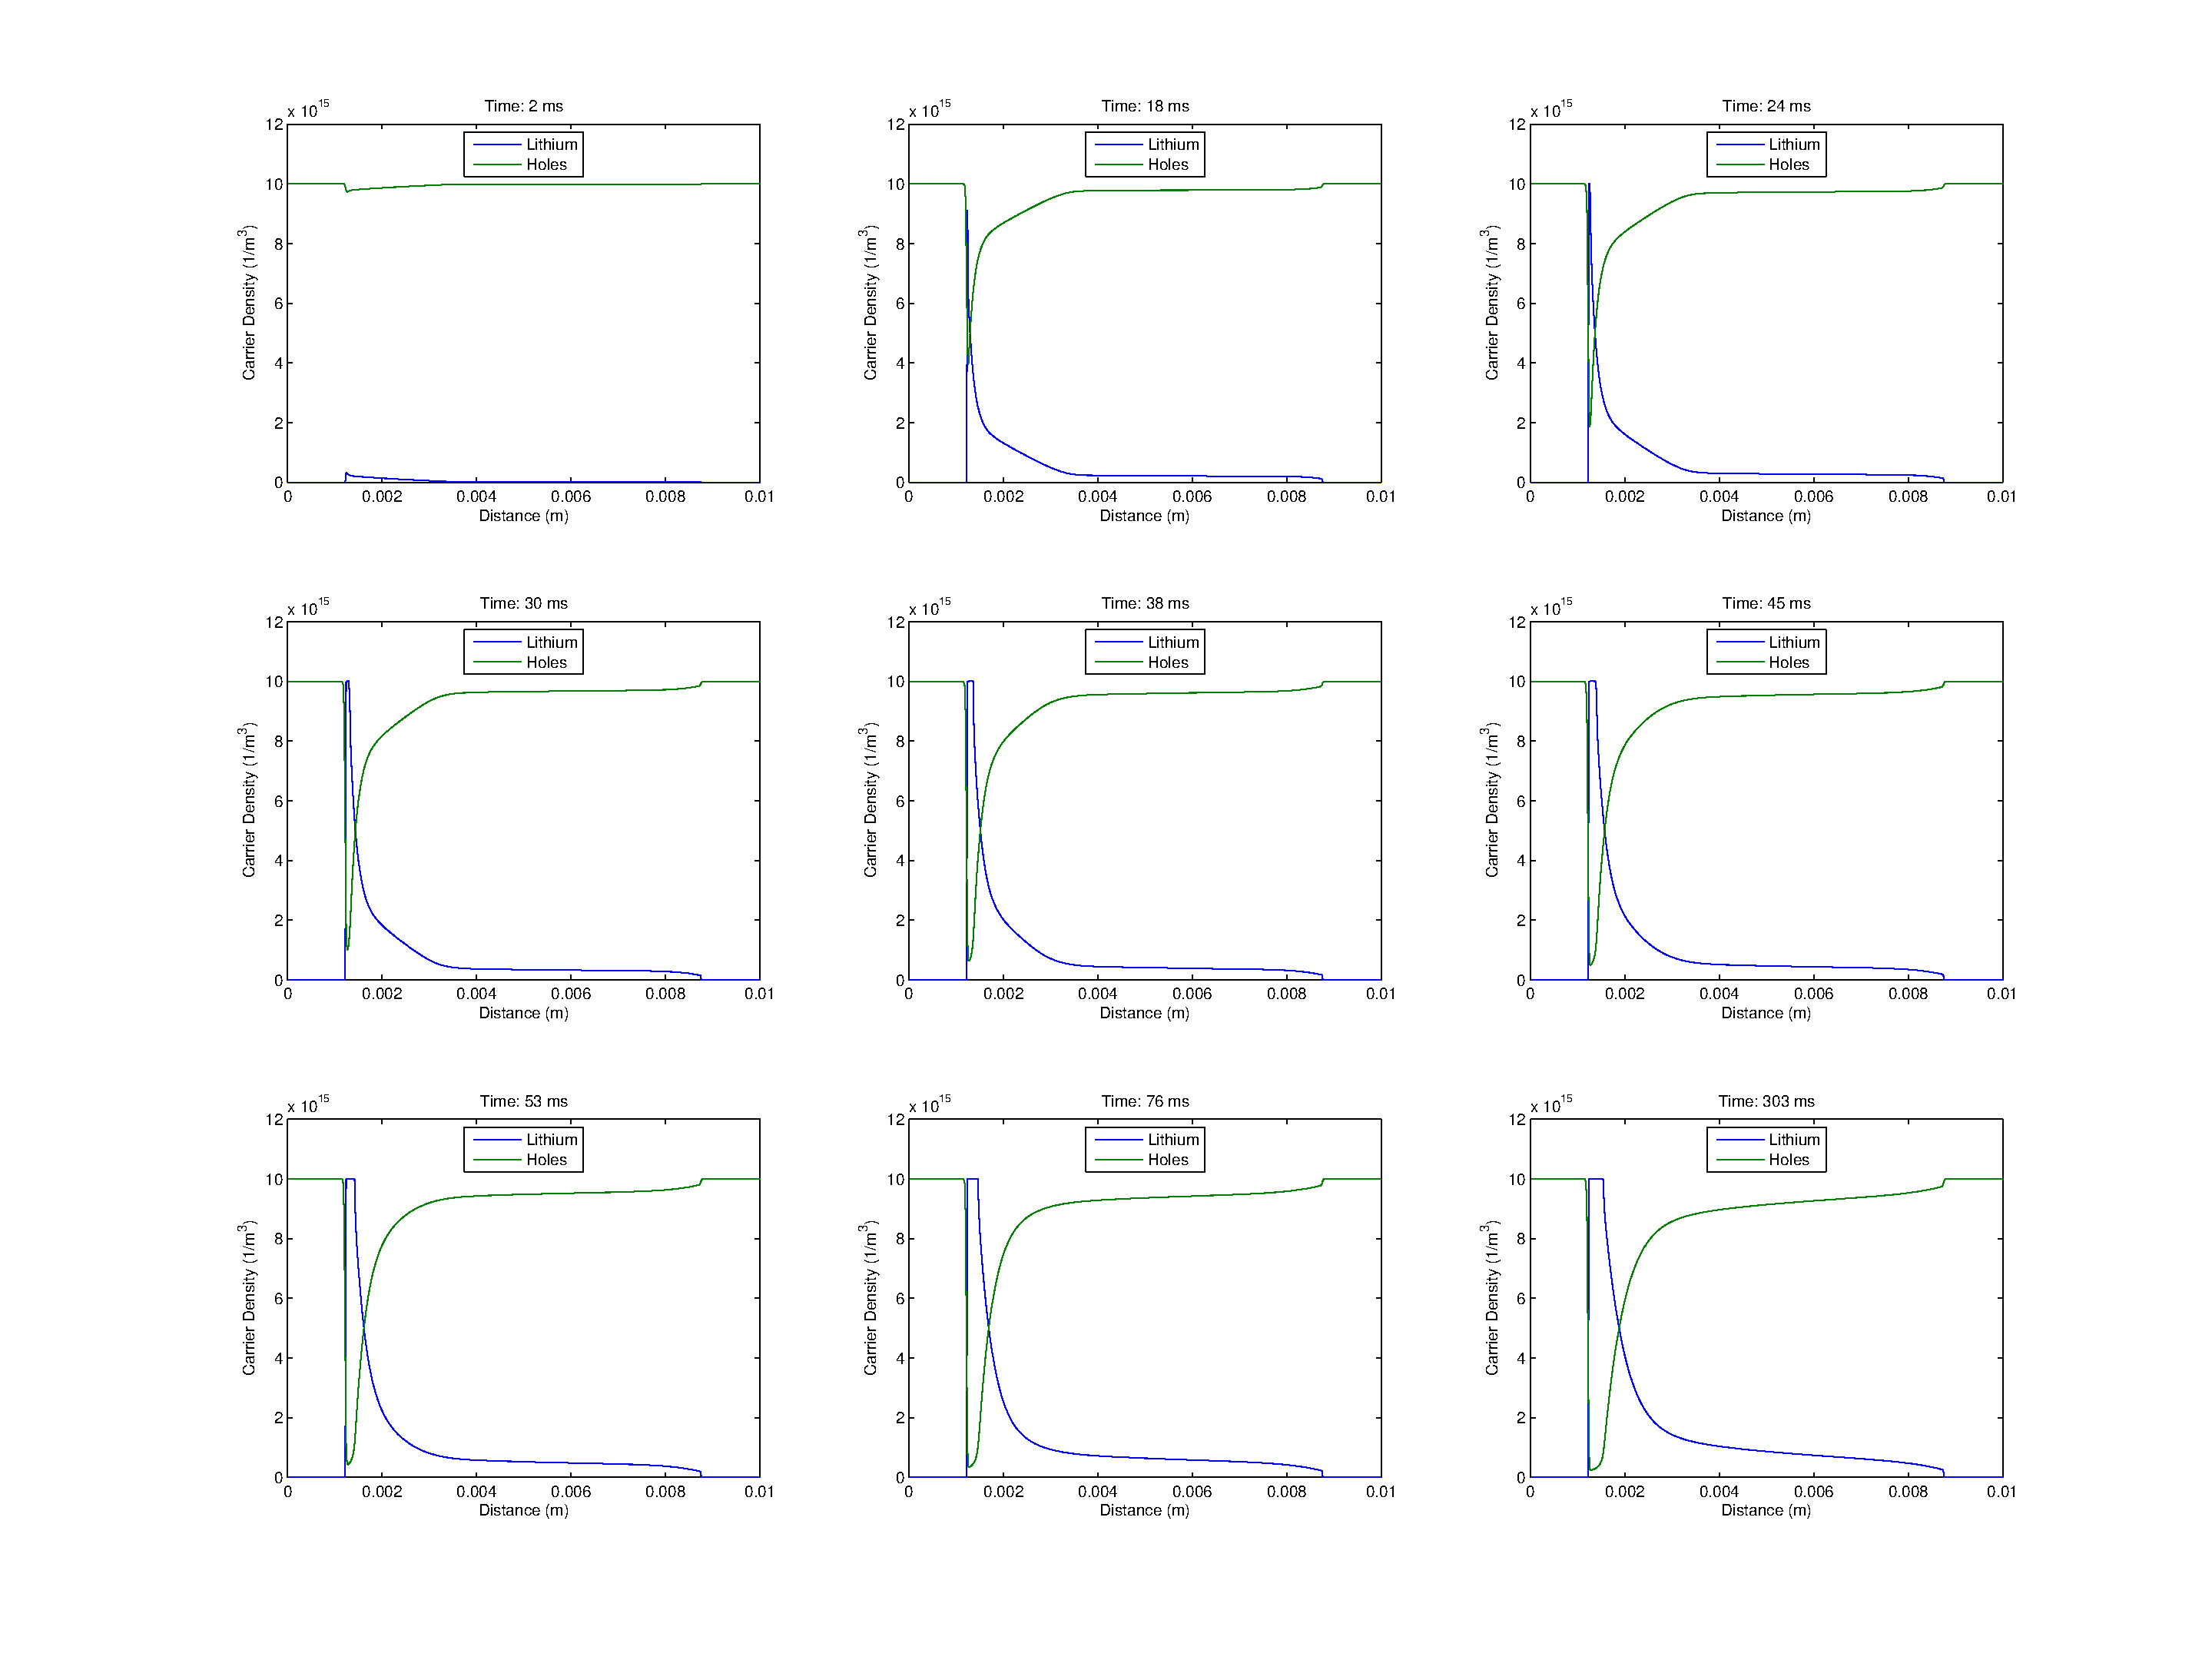
\includegraphics[scale=0.40]{Ex5pNp_Time1}
\caption{} 
\label{}
\end{figure}
\end{landscape}

\begin{landscape}
\begin{figure}[!htp]
\centering
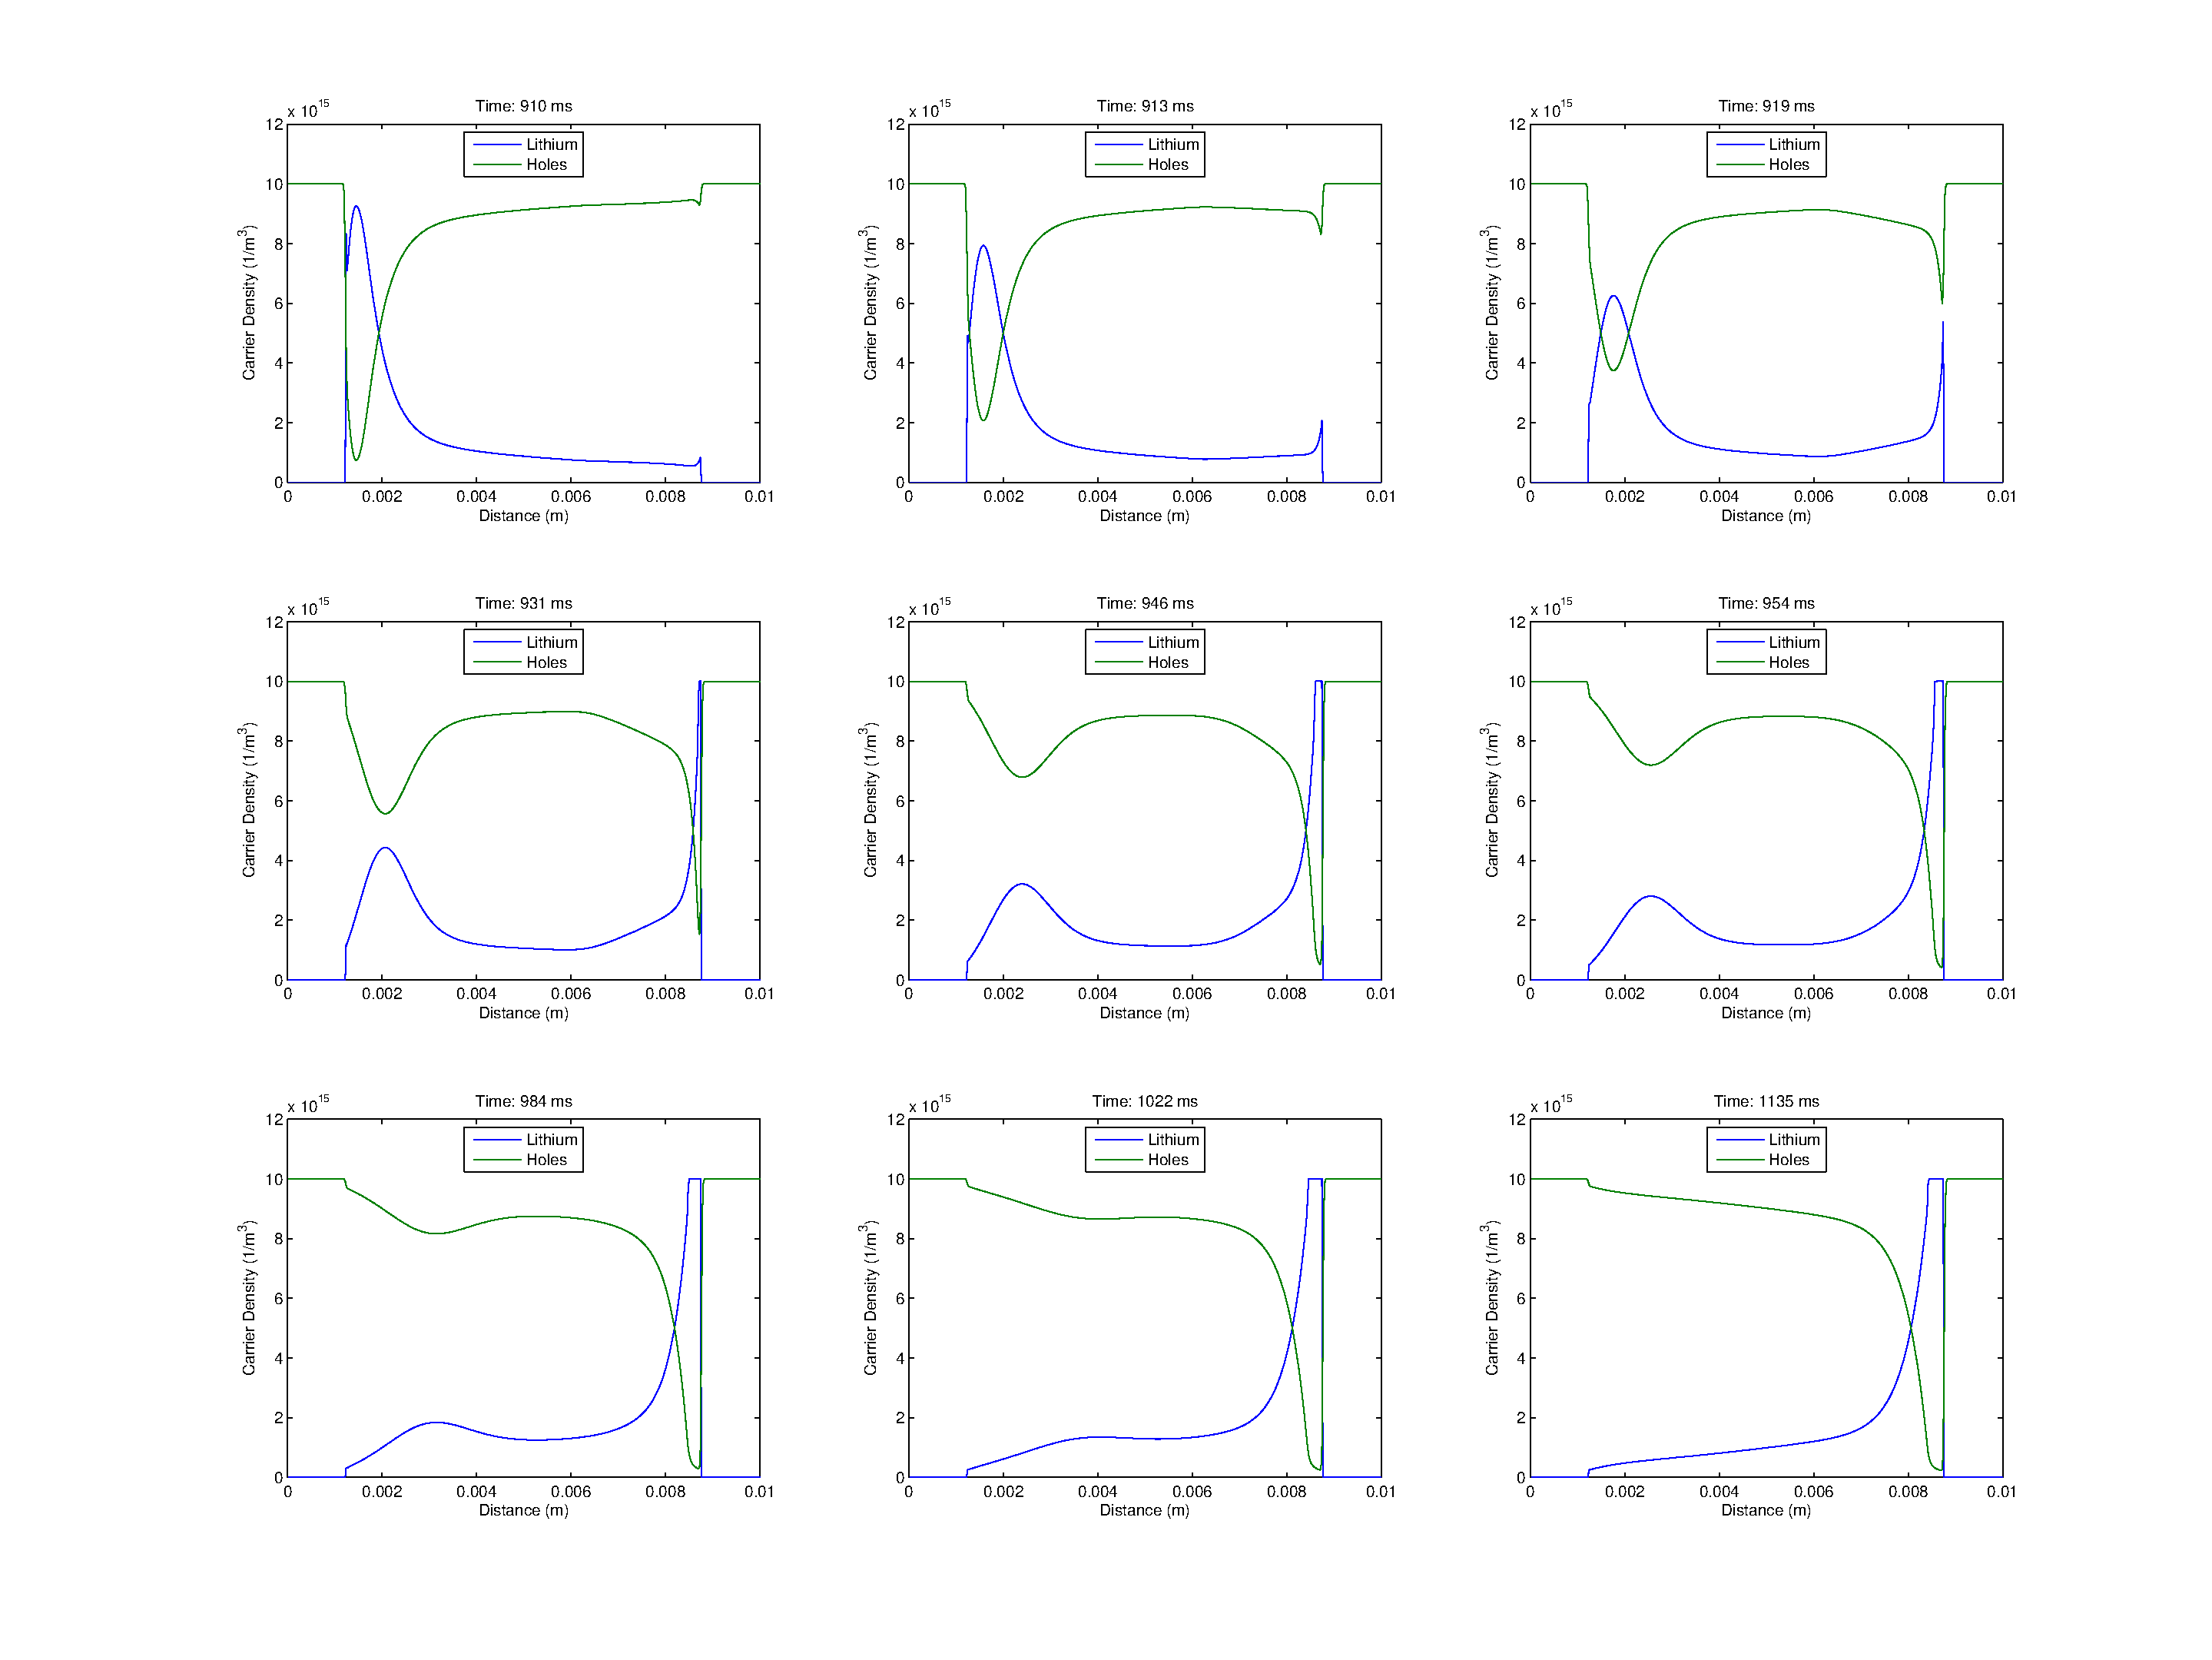
\includegraphics[scale=0.40]{Ex5pNp_Time2}
\caption{} 
\label{}
\end{figure}
\end{landscape}



\begin{figure}[!htp]
\centering
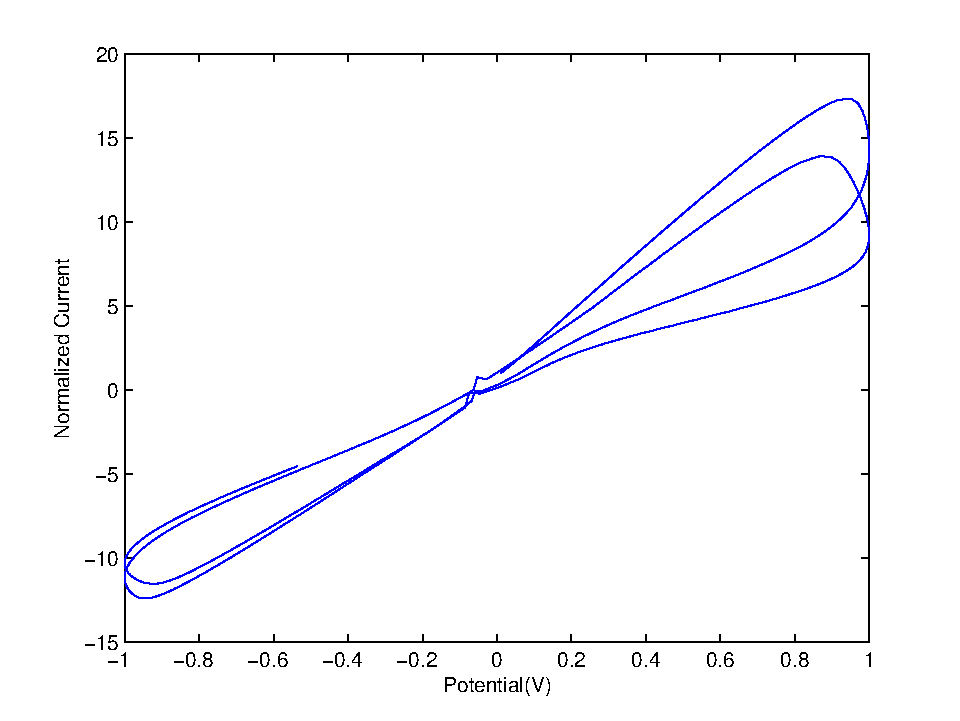
\includegraphics[scale=0.60]{Ex5Bowtie}
\caption{} 
\label{}
\end{figure}


%1-D Vertical Medium and high concentration (hole freeze,# of holes over time)
%1-D Horizontal medium and high concentration (Add memristor pictures,hole freeze,# of holes over time)
